%%%%%%%%%%%%%%%%%%%%%%%%%%%%%%%%%%%%%%%%%
% Masters/Doctoral Thesis 
% LaTeX Template
% Version 2.3 (25/3/16)
%
% This template has been downloaded from:
% http://www.LaTeXTemplates.com
%
% Version 2.x major modifications by:
% Vel (vel@latextemplates.com)
%
% This template is based on a template by:
% Steve Gunn (http://users.ecs.soton.ac.uk/srg/softwaretools/document/templates/)
% Sunil Patel (http://www.sunilpatel.co.uk/thesis-template/)
%
% Template license:
% CC BY-NC-SA 3.0 (http://creativecommons.org/licenses/by-nc-sa/3.0/)
%
%%%%%%%%%%%%%%%%%%%%%%%%%%%%%%%%%%%%%%%%%

%----------------------------------------------------------------------------------------
%	PACKAGES AND OTHER DOCUMENT CONFIGURATIONS
%----------------------------------------------------------------------------------------

\documentclass[
11pt, % The default document font size, options: 10pt, 11pt, 12pt
oneside, % Two side (alternating margins) for binding by default, uncomment to switch to one side
%chapterinoneline,% Have the chapter title next to the number in one single line
english, % ngerman for German
onehalfspacing, % Single line spacing, alternatives: onehalfspacing or doublespacing
%draft, % Uncomment to enable draft mode (no pictures, no links, overfull hboxes indicated)
%nolistspacing, % If the document is onehalfspacing or doublespacing, uncomment this to set spacing in lists to single
liststotoc, % Uncomment to add the list of figures/tables/etc to the table of contents
%toctotoc, % Uncomment to add the main table of contents to the table of contents
%parskip, % Uncomment to add space between paragraphs
%nohyperref, % Uncomment to not load the hyperref package
headsepline, % Uncomment to get a line under the header
]{MastersDoctoralThesis} % The class file specifying the document structure

\usepackage[utf8]{inputenc} % Required for inputting international characters
\usepackage[T1]{fontenc} % Output font encoding for international characters

\usepackage{palatino} % Use the Palatino font by default

\usepackage[backend=bibtex]{biblatex} %,style=authoryear,natbib=true]{biblatex} % Use the bibtex backend with the authoryear citation style (which resembles APA)

\addbibresource{predicting.bib} % The filename of the bibliography

\usepackage[autostyle=true]{csquotes} % Required to generate language-dependent quotes in the bibliography

\usepackage{tikz}
\usetikzlibrary{shapes, backgrounds}

% page number on first page of bibliography
\renewcommand{\bibsetup}{\thispagestyle{nohead}\pagestyle{thesis}}

%----------------------------------------------------------------------------------------
%	MARGIN SETTINGS
%----------------------------------------------------------------------------------------

\geometry{
	paper=a4paper, % Change to letterpaper for US letter
	inner=2.5cm, % Inner margin
	outer=3.8cm, % Outer margin
	bindingoffset=2cm, % Binding offset
	top=1.5cm, % Top margin
	bottom=1.5cm, % Bottom margin
	%showframe,% show how the type block is set on the page
}

%----------------------------------------------------------------------------------------
%	THESIS INFORMATION
%----------------------------------------------------------------------------------------

\thesistitle{Predicting SMT solver performance for software verification} % Your thesis title, this is used in the title and abstract, print it elsewhere with \ttitle
\supervisor{Dr. James F. \textsc{Power}\\ Dr. Rosemary \textsc{Monahan}} % Your supervisor's name, this is used in the title page, print it elsewhere with \supname
\examiner{} % Your examiner's name, this is not currently used anywhere in the template, print it elsewhere with \examname
\degree{Master of Science} % Your degree name, this is used in the title page and abstract, print it elsewhere with \degreename
\author{Andrew \textsc{Healy}} % Your name, this is used in the title page and abstract, print it elsewhere with \authorname
\addresses{} % Your address, this is not currently used anywhere in the template, print it elsewhere with \addressname

\subject{Computer Science} % Your subject area, this is not currently used anywhere in the template, print it elsewhere with \subjectname
\keywords{} % Keywords for your thesis, this is not currently used anywhere in the template, print it elsewhere with \keywordnames
\university{Maynooth University} % Your university's name and URL, this is used in the title page and abstract, print it elsewhere with \univname
\department{Department of Computer Science} % Your department's name and URL, this is used in the title page and abstract, print it elsewhere with \deptname
\group{Principles of Programming Research Group} % Your research group's name and URL, this is used in the title page, print it elsewhere with \groupname
\faculty{Faculty of Science and Engineering} % Your faculty's name and URL, this is used in the title page and abstract, print it elsewhere with \facname
\hypersetup{pdftitle=\ttitle} % Set the PDF's title to your title
\hypersetup{pdfauthor=\authorname} % Set the PDF's author to your name
\hypersetup{pdfkeywords=\keywordnames} % Set the PDF's keywords to your keywords

\begin{document}

\frontmatter % Use roman page numbering style (i, ii, iii, iv...) for the pre-content pages

\pagestyle{nohead} % Default to the plain heading style until the thesis style is called for the body content

%----------------------------------------------------------------------------------------
%	TITLE PAGE
%----------------------------------------------------------------------------------------

\begin{titlepage}
\begin{center}


\includegraphics[width=30mm]{MULogo} % University/department logo - uncomment to place it
\HRule \\[0.4cm] % Horizontal line
{\huge \bfseries \ttitle\par}\vspace{0.4cm} % Thesis title
\HRule \\[1.5cm] % Horizontal line
{\huge \authorname}\vspace{0.6cm}

\large \textit{A thesis submitted in partial fulfillment of the requirements\\ for the degree of }\degreename\\[0.3cm]\vspace{0.8cm} % University requirement text

{\scshape\Large \univname}\vspace{0.8cm} \\ % University name
\deptname\\\facname\\[2cm] % Research group name and department name
October 2016\\ 
\vfill
\begin{minipage}[t]{0.4\textwidth}
\begin{flushleft} \large
\emph{Head of Department:} \\
Dr. Adam \textsc{Winstanley}
\end{flushleft}
\end{minipage}
\begin{minipage}[t]{0.4\textwidth}
\begin{flushright} \large
\emph{Supervisors:} \\
\supname % Supervisor name - remove the \href bracket to remove the link  
\end{flushright}
\end{minipage}\\[3cm]

\end{center}
\end{titlepage}

%----------------------------------------------------------------------------------------
%	LIST OF CONTENTS/FIGURES/TABLES PAGES
%----------------------------------------------------------------------------------------
\pagestyle{nohead}
\tableofcontents % Prints the main table of contents

%
%%----------------------------------------------------------------------------------------
%%	DECLARATION PAGE
%%----------------------------------------------------------------------------------------
%
%\begin{declaration}
%\addchaptertocentry{\authorshipname}
%
%\noindent I, \authorname, declare that this thesis titled, \enquote{\ttitle} and the work presented in it are my own. I confirm that:
%
%\begin{itemize} 
%\item This work was done wholly or mainly while in candidature for a research degree at this University.
%\item Where any part of this thesis has previously been submitted for a degree or any other qualification at this University or any other institution, this has been clearly stated.
%\item Where I have consulted the published work of others, this is always clearly attributed.
%\item Where I have quoted from the work of others, the source is always given. With the exception of such quotations, this thesis is entirely my own work.
%\item I have acknowledged all main sources of help.
%\item Where the thesis is based on work done by myself jointly with others, I have made clear exactly what was done by others and what I have contributed myself.\\
%\end{itemize}
% 
%\noindent Signed:\\
%\rule[0.5em]{25em}{0.5pt} % This prints a line for the signature
% 
%\noindent Date:\\
%\rule[0.5em]{25em}{0.5pt} % This prints a line to write the date
%\end{declaration}
%
%\cleardoublepage

%----------------------------------------------------------------------------------------
%	QUOTATION PAGE
%----------------------------------------------------------------------------------------

%\vspace*{0.2\textheight}

%\noindent\enquote{\itshape Thanks to my solid academic training, today I can write hundreds of words on virtually any topic without possessing a shred of information, which is how I got a good job in journalism.}\bigbreak

%\hfill Dave Barry

%----------------------------------------------------------------------------------------
%	ABSTRACT PAGE
%----------------------------------------------------------------------------------------

\begin{abstract}
\addchaptertocentry{\abstractname} % Add the abstract to the table of contents

The approach \why takes to interfacing with a wide variety of interactive and automatic theorem provers works well: it is designed to overcome limitations on what can be proved by a system which relies on a single tightly-integrated solver. In common with other systems, however, the degree to which proof obligations (or ``goals'') are proved depends as much on the SMT solver as the properties of the goal itself. In this work, we present a method to use syntactic analysis to characterise goals and predict the most appropriate solver via machine-learning techniques.  

Combining solvers in this way - a \textit{portfolio-solving} approach - maximises the number of goals which can be proved. The driver-based architecture of \why presents a unique opportunity to use a portfolio of SMT solvers for software verification. The intelligent scheduling of solvers minimises the time it takes to prove these goals by avoiding solvers which return \textit{Timeout} and \textit{Unknown} responses. We assess the suitability of a number of machine-learning algorithms for this scheduling task.  

The performance of our tool \where is evaluated on a large dataset of proof obligations. We compare \where to a range of SMT solvers and theoretical scheduling strategies. We find that \where can prove a greater number of goals in a shorter amount of time than any single solver. Furthermore, \where can integrate into a \why user's normal workflow - simplifying and automating the use of SMT solvers for software verification. 

\end{abstract}

%----------------------------------------------------------------------------------------
%	ACKNOWLEDGEMENTS
%----------------------------------------------------------------------------------------

\begin{acknowledgements}
\addchaptertocentry{\acknowledgementname} % Add the acknowledgements to the table of contents

The acknowledgments and the people to thank go here, don't forget to include your project adviser\ldots

\end{acknowledgements}


%----------------------------------------------------------------------------------------
%	ABBREVIATIONS
%----------------------------------------------------------------------------------------

\begin{abbreviations}{ll} % Include a list of abbreviations (a table of two columns)
\thispagestyle{nohead}
\textbf{ATP} & \textbf{A}utomatic \textbf{T}heorem \textbf{P}rover \\
\textbf{DSL} & \textbf{D}omain \textbf{S}pecific \textbf{L}anguage \\
\textbf{IDE} & \textbf{I}ntegrated \textbf{D}evelopment \textbf{E}nvironment \\
\textbf{ITP} & \textbf{I}nteractive \textbf{T}heorem \textbf{P}rover \\
\textbf{PO} & \textbf{P}roof \textbf{O}bligation \\
\textbf{SAT} & \textbf{Sat}isfiability \\
\textbf{SE} & \textbf{S}oftware \textbf{E}ngineering \\
\textbf{SMT(-LIB)} & \textbf{S}atisfiability \textbf{M}odulo \textbf{T}heories (-\textbf{Lib}rary) \\
\textbf{SV} & \textbf{S}oftware \textbf{V}erification

\end{abbreviations}

\listoffigures % Prints the list of figures
\thispagestyle{nohead}

\listoftables % Prints the list of tables
\thispagestyle{nohead}
%----------------------------------------------------------------------------------------
%	DEDICATION
%----------------------------------------------------------------------------------------

%\dedicatory{For/Dedicated to/To my\ldots} 

%----------------------------------------------------------------------------------------
%	THESIS CONTENT - CHAPTERS
%----------------------------------------------------------------------------------------

\mainmatter % Begin numeric (1,2,3...) page numbering

\pagestyle{thesis} % Return the page headers back to the "thesis" style

% Include the chapters of the thesis as separate files from the Chapters folder
% Uncomment the lines as you write the chapters

% Chapter 1

\chapter{Introduction} % Main chapter title
\thispagestyle{nohead}
\label{Intro} % For referencing the chapter elsewhere, use \ref{Intro} 

%----------------------------------------------------------------------------------------

% Define some commands to keep the formatting separated from the content 
\newcommand{\keyword}[1]{\textbf{#1}}
\newcommand{\tabhead}[1]{\textbf{#1}}
\newcommand{\code}[1]{\texttt{#1}}
\newcommand{\file}[1]{\texttt{\bfseries#1}}
\newcommand{\option}[1]{\texttt{\itshape#1}}
%----------------------------------------------------------------------------------------
The necessity of software verification (SV) has been demonstrated by numerous failures. 
Some of these failures have

Software faults can have disastrous consequences 
As the complexity of software projects increases

\section{Software Verification Background}
\subsection{Software Verification Systems as Composed of Modular Components}
\subsection{The \why~system}
\subsubsection{Front End: \why~as an intermediary language}
\subsubsection{Back End: Driver-based interface to \textsc{APT}, \textsc{ITP} and \textsc{SMT} tools}
\subsection{An overview of various \textsc{SMT} solvers and their capabilities}
\section{Problem Statement}

The efficient allocation of SMT-solving resources for software verification tasks

\section{Contributions}
The main contributions of this work are:
\begin{enumerate}
	\item The design  and implementation of our portfolio solver, \textsf{Where4}, which uses supervised machine learning to predict the best solver to use based on metrics collected from goals.
	\item The integration of \textsf{Where4} into the user's existing \textsf{Why3} work-flow by imitating the behaviour of an orthodox SMT solver.
	\item A set of metrics to characterise \textsf{Why3} goal formulae.
	\item Statistics on the performance of eight SMT solvers using a dataset of 1048 \textsf{Why3} goals.
	
\end{enumerate}

%\section{The benefits of a portfolio-based approach to software verification}
\begin{figure}
\centering
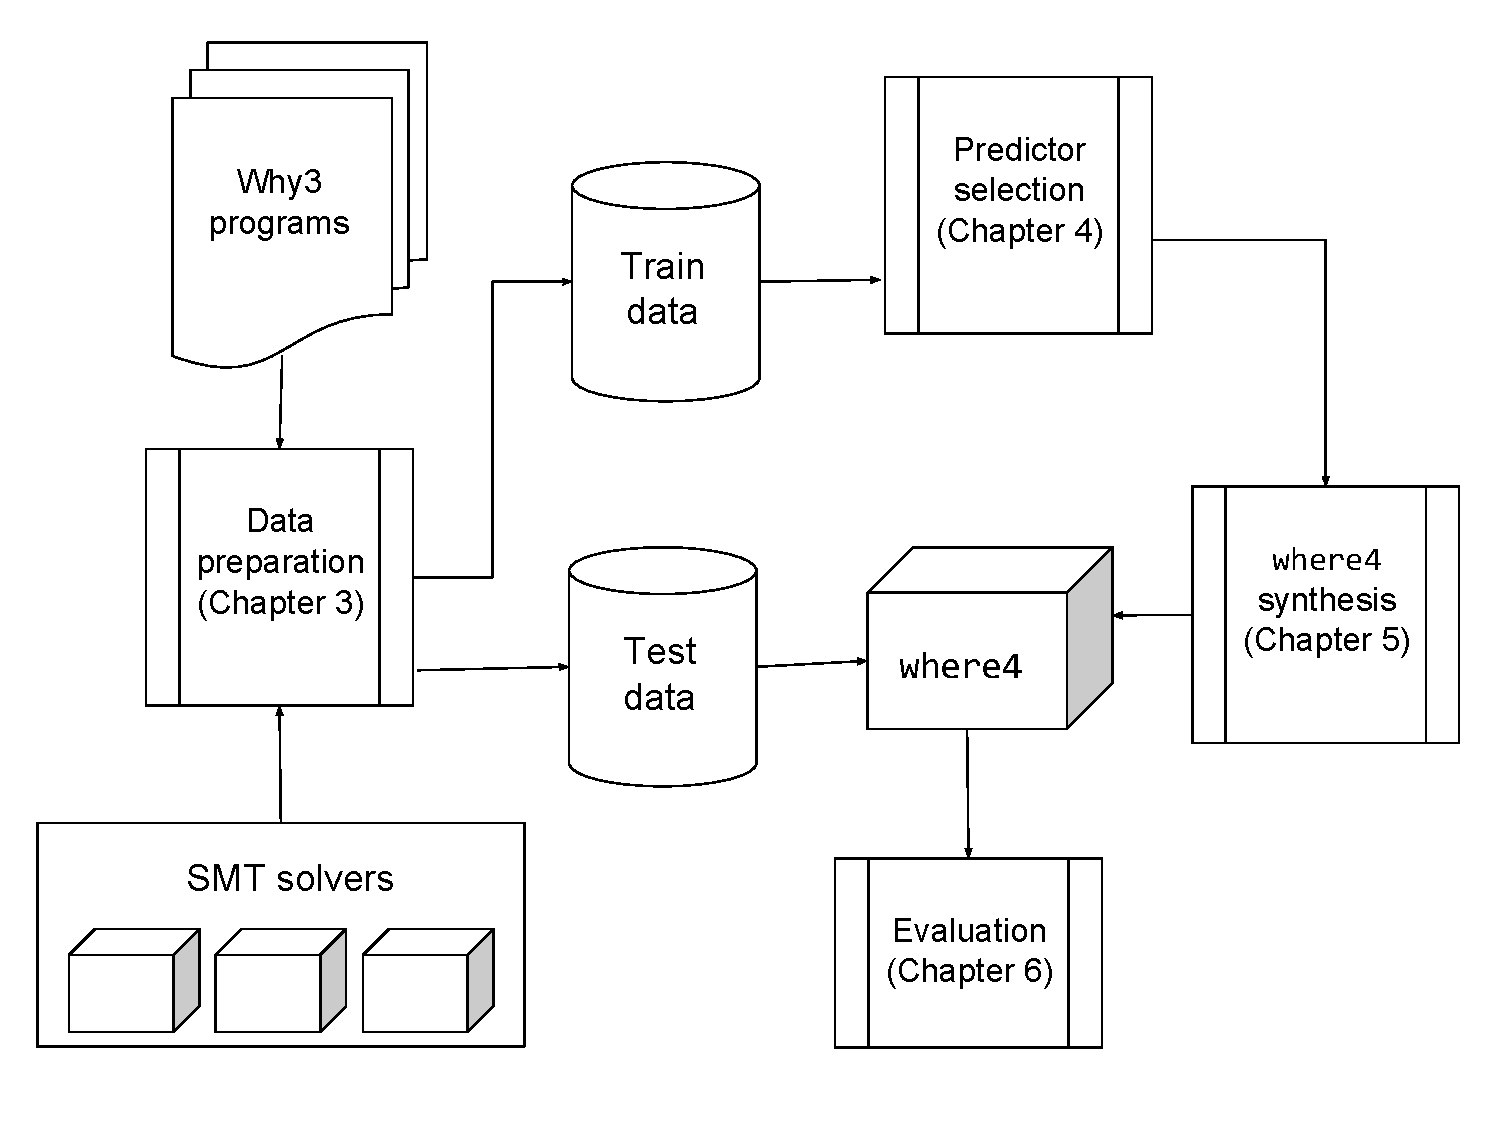
\includegraphics[width=0.9\linewidth]{Figures/intoduction}
\caption{Overview of the \where~project and this thesis's structure}
\label{fig:introduction}
\end{figure}


\chapter{Literature Review}% Main chapter title
\thispagestyle{nohead}
\label{LitReview} % For referencing the chapter elsewhere, use \ref{LitReview} 

%----------------------------------------------------------------------------------------

This chapter views \where~as incorporating ideas from three separate disciplines: software verification, machine learning, and software measurement and metrics. 
%Each of these disciplines has a considerable body of research associated with it.
A Venn diagram illustrating the intersections of these disciplines and how this chapter is organised according to these intersections is given in Fig. \ref{fig:litreview}. 
We shall concentrate this review on Software Verification and SV research incorporating concepts from the other two disciplines. 
Where more background in associated topics outside the SV domain is required, the literature is discussed in the relevant sections (i.e. Sec. \ref{sec:lrmm} and \ref{sec:lrml}).

The rest of this chapter will review the literature associated with each segment of Figure \ref{fig:litreview} -- moving clockwise from the top. 
Each subsection in this review was approached with a question:
\begin{itemize}
	\item[\textbf{Q1}] What does the SV tool landscape look like in terms of interoperability?
	\item[\textbf{Q2}] Does a standardised suite of benchmark programs exist for the comparison of deductive SV tools?
	\item[\textbf{Q3}] How have concepts from traditional SE been applied to large-scale SV projects?
	\item[\textbf{Q4}] How have machine learning concepts been integrated for use in the SV domain?
\end{itemize}
the answers of which have informed the design choices made in regard to the \where~portfolio-solving tool.

\begin{figure}

\centering
\def\firstcircle{(3cm,0cm) circle (2.5cm)}
\def\secondcircle{(0cm,0cm) circle (2.5cm)}
\def\thirdcircle{(1.5cm,3cm) circle (2.5cm)}
\begin{tikzpicture}
	
	\draw \firstcircle node [below] {};
	\draw \secondcircle node [above] {};
	\draw \thirdcircle node [below] {};
	\node[align=center] at (-1cm, 0cm) {Machine\\Learning\\ \ref{sec:lrml} };
	\node[align=center] at (1.5cm, 4cm) {Software\\Verification\\ \ref{sec:lrsv}};
	\node[align=center] at (4cm, 0cm) {Metrics \&\\ Measurement\\ \ref{sec:lrmm}};
	\node[align=center] at (1.5cm, 1.2cm) {\ref{sub:lrsvmmml}\\\small{\where} };
	\node[align=center] at (0.3cm, 1.6cm) {\ref{sub:lrsvml}};
	\node[align=center] at (2.7cm, 1.6cm) {\ref{sub:lrsvmm}};
	\node[align=center] at (1.5cm, -0.5cm) {\ref{sub:lrmmml}};
	
\end{tikzpicture}

\caption{\where~as placed at the intersection of three disciplines}
\label{fig:litreview}

\end{figure}


\section{\why~and Software Verification Systems}
\label{sec:lrsv}

An overview of the \why~verification system \cite{why:shephard,why:whereprovers} has been given in the previous chapter. The WhyML programming language provides a high-level ML\footnote{The ML language -- not to be confused with \underline{M}achine \underline{L}earning}-like language for the specification of programs with pre- and post- conditions, recursive definitions and type invariants. An extensive library of verified polymorphic data-types make WhyML a flexible language \cite{verifythis,why:polymorphic}. 
As we stated in the previous chapter, it is \why's driver-based approach to interfacing with external tools that is of most interest to our project. 
The \why~approach is, in this regard, quite different from the typical SV system of tightly-integrated systems consisting of an IDE/annotation language/front-end DSL, intermediate logic language, and SMT-solving back-end. 
Examples of systems which follow this latter model are Spec\# \cite{spec} and Dafny \cite{Dafny} which use the Boogie \cite{Boogie} intermediate language and the Z3 \cite{Z3} SMT solver.

The diversity of languages and formalisms has been matched by an increase in software verification \textit{tools} in recent years. 
Filli{\^a}tre's overview of the deductive verification tool landscape \cite{deductiveSV} counts 65 tools cited or used in the five papers of a special edition of the \textit{Verified Software: Theory, Tools and Experiments} post-proceedings in 2009. 
Recently, there has been an effort to make these tools more interoperable. 
The two-dozen ATPs, ITPs and SMT solvers targeted by \why~make it an attractive choice for translations: recent projects have used \why~as a platform for discharging POs translated from Boogie \cite{b2w} and the B system \cite{rodinplugin,atelierB2w}. \\

\textbf{Q1: What does the SV tool landscape look like in terms of interoperability?} \\
\why~is clearly the most open platform for software verification; integrating as it does the use of ATPs, SMT solvers and ITPs.
We chose the \why~system for the flexibility of its specification language, extensible driver-based architecture and potential for conducting a comparative evaluation of several theorem-proving tools.

\subsection{Measurement and Metrics in Software Verification}
\label{sub:lrsvmm}

With the diversity of languages, formats, and approaches currently in use in the SV domain, experimental software measurement concepts and techniques must be introduced for the rigorous evaluation, comparison, and characterisation of software. These techniques are usually employed in the general software engineering domain and have been adapted for the specific concerns of formal methods. 

The intersection of SV and empirical SE disciplines can be further broken into the two subsections to follow. 
Benchmark repositories and tool competitions have proven to be important as a means of evaluation and improvement among SV communities. A number of large-scale SV projects, meanwhile, have necessitated the adaptation of established SE metrics and methodologies.         
 
\begin{table}
	\caption[Summary of SV benchmark sources]{Summary of SV benchmark sources}
	\begin{adjustbox}{angle=90}  
	\begin{tabularx}{0.9\textheight}{@{}Y|Y|Y|Y|Y|Y|c@{}}
		\textsc{\textbf{Benchmark Source}} & \textsc{\textbf{Target Domain}} &  \textsc{\textbf{Example tools}} & \textsc{\textbf{Input format}} & \textsc{\textbf{Size}} & \textsc{\textbf{Website}} \linebreak \small{(last visited 28/9/16)} & \textsc{\textbf{Reference}} \\
		\midrule
		VerifyThis & Program Verification Systems & \why, Dafny, Spec\#, VeriFast, KIV & Natural Language and Pseudo Code & 33 & \href{http://www.verifythis.org/challenge-db}{verifythis.org} & \cite{Huisman2015} \\ 
		\midrule
		VSTTE Incremental Benchmarks & Program Verification Systems & \why, Dafny, RESOLVE & Natural Language & 8 & - & \cite{Weide2008} \\ 
		\midrule
		VACID-0 & Program Verification Systems & \why, Dafny, KeY, VCC, Coq & Natural Language and Pseudo Code & 5 & - & \cite{Leino10vacid-0:verification} \\
		\midrule
		SMT-LIB & SMT solvers & Z3, CVC4, Yices2, veriT, Alt-Ergo & SMT-LIB v2 & > 100,000 POs & \href{http://smtlib.cs.uiowa.edu/benchmarks.shtml}{smtlib.org} & \cite{BarFT-SMTLIB} \\
		\midrule
		TPTP & ATPs and SMT solvers & \why, Eprover, Beagle, CVC3, CVC4 & TPTP & 20,306 POs & \href{http://www.cs.miami.edu/~tptp}{tptp.org} & \cite{SS98} \\
		\midrule
		BWARE & ATPs and SMT solvers & \why, Alt-Ergo, CVC3, CVC4 & TPTP / SMT-LIB v2 & 12,876 POs & \href{http://bware.lri.fr/index.php/Benchmarks}{bware.lri.fr} & \cite{Delahaye2014} \\
		\midrule
		SV-COMP & ATPs and model-checkers & AProVE, BLAST, CPAchecker & C & 6661 files & \href{http://sv-comp.sosy-lab.org}{sv-comp.sosy-lab.org} & \cite{SVCOMP} \\   
		\midrule
		The \why~examples & Program verification through \why & \why~and its supported back-ends & WhyML & 128 programs, 1048 POs & \href{http://tocatta.lri.fr/gallery/why3.en.html}{toccata.lri.fr} & \cite{verifythis, tafat:inria-00636083} \\
		
	\end{tabularx}
	\end{adjustbox}
	\label{table:benchmarks}
\end{table}


\subsubsection{Software Verification Competitions and Benchmark Repositories}
\label{sub:lrsvmmbench}

At present, competitions provide the most prominent means of comparing systems which focus on the verification of object-oriented software. 
In competitions such as those held at FoVeOOS 2011 \cite{bormer:hal-00789525} and the VerifyThis series \cite{Huisman2015}, teams are given the natural-language specifications and pseudo-code for a small number of typical SV problems. 
Any system can be used, with tool developers often choosing to compete using their own system. 
As well as evaluating solutions based on correctness and completeness, an emphasis is placed on judging a team's implementation \textit{approach} and \textit{ideas}, given the diverse capabilities of the SV systems in use. 
Previous challenges have been based on a set of 8 incremental benchmarks for software verification tools proposed by Weide et al. at VSTTE 2008 \cite{Weide2008}. The \why~development team are regular competitors at VerifyThis and some of the standard \why~examples are refined versions of solutions submitted at the competition \cite{verifythis}.  

%  Many of the \why gallery of verified programs originated from software verification competitions \cite{verifythis, tafat:inria-00636083}.  

SV-COMP \cite{Beyer2016, SVCOMP} is a well-established annual competition for automatic program verifiers. 
The tools use static analysis and model-checking techniques to ensure properties such as reachability or termination. 
Teams can choose to compete in a subset of categories based on the strengths of their tool. 
As soundness of automatic program verifiers cannot be guaranteed, marks are deducted for false positive and false negative answers. 
The scoring hierarchy rewards true positive answers with the highest marks and penalises false positive answers severely; with ``Unknown'' answers having zero effect on a tool's score.
We followed a similar scoring hierarchy when devising \where's cost function (Sec. \ref{sub:scoring}).
 
Importantly, a large, publicly-available benchmark repository consisting of 6661 programs  has been developed using these competition questions. It is possible to maintain such a repository due to the standard input format of the tools which all accept input in the C language. Other efforts to standardise benchmark repositories for software verification tools are discussed in the next subsection and summarised in Table \ref{table:benchmarks}.  

The need for a standard set of benchmarks for the diverse range of verification systems was identified by a number of participants in the week-long seminar at Dagstuhl \cite{Dagstuhl} in 2014. The series of workshops and events brought the model-checking and SV system communities together. Qualitative, repeatable comparative evaluation was agreed as an important goal if deductive software verification is to advance as an engineering discipline. Following on form the 8 incremental benchmarks proposed at VSTTE referenced in the previously, the VACID-0 \cite{Leino10vacid-0:verification} project is another attempt to maintain a repository of standard abstract specifications for verified data structures and operations similar to those used in the VerifyThis competition. The VACID-0 benchmarks also include a marking scheme to identify the most important aspects of the specification for a tool to be able to verify.

In addition to SV-COMP, the benefits of a large benchmark suite written in a common input language are evidenced by the SMT-LIB \cite{SMTLIB} project. 
The performance of SMT solvers has significantly improved in recent years due in part to the standardisation of an input language and the use of standard benchmark programs in competitions \cite{SMTEVAL2013}. 
In contrast to the ATPs competing in SV-COMP, SMT solvers are assumed to be correct. Therefore, solvers are marked according to how many problems can be solved and the time taken to solve problems.
\why~includes a SMT-LIB printer and uses the format for a number of SMT solvers (including CVC4, Z3, and veriT). Our previous work \cite{Healy:2016} has exploited this feature: verification tasks were compared to other application domains of SMT solvers using the SMT-LIB repository as a data source.

The TPTP (Thousands of Problems for Theorem Provers) project \cite{TPTP} is a benchmark repository with similar aims to SMT-LIB but a wider scope. The problems target theorem provers which specialise in numerical problems as well as general-purpose SAT and SMT solvers. The TPTP library is specifically designed for the rigorous experimental comparison of solvers \cite{Sutcliffe200139}. There has been significant development effort by \why~developers to support the TPTP format in \why~and to extend the TPTP language with rank-1 polymorphism \cite{why:tptp} thereby allowing the use of ML-like polymorphic types to be used in an interchange format understood by over two-dozen provers. This extension of the TPTP language makes it more similar to the specification language of \why.   \\

\textbf{Q2: Does a standardised suite of benchmark programs exist for the comparison of deductive SV tools?} \\
Although the need for such a benchmark suite is well understood, the diversity of input languages hampers progress towards this goal. 
A small number of abstract specifications for standard problems, mostly collected by competitions which evaluate \textit{approaches} used by various systems to software verification, are the closest approximation.  

\subsubsection{Proof Engineering}
\label{sub:lrsvmmpe}

The scale of formal software engineering projects has grown in recent years. The formal verification of the seL4 microkernel \cite{Klein:2014:CFV} and Thomas Hales' \textit{FlySpeck} proof of the Kepler Conjecture \cite{hales-kepler} are large and complicated engineering projects developed over a number of years. Both projects represent significant engineering efforts -- it is estimated that the seL4 verification took 25 person-years of work -- and produced a large volume of software artefacts in the form of \textit{proof scripts}. Researchers applying concepts from software engineering to manage and measure such projects call their practice ``proof engineering'' \cite{Klein2014}. Proof engineering is has become an active research area in recent years. 

Both object-oriented software and formal proofs make use of ``modules'' to package related classes and lemmas/axioms respectively. Aspinall and Kaliszyk \cite{Aspinall2016} suggest that this common approach to modularity allows the standard Chidamber and Kemerer \cite{CandK} (CK) metrics to be adapted for formal SE projects. The authors use this analogy to model and measure the dependency tree for proof modules and the derivation of the module's coupling and cohesion metrics (CK metrics will be discussed further in Section \ref{sec:lrmm}).

Other approaches measure syntactic features of the specification to derive complexity metrics. The verification of the seL4 microkernel mentioned previously was used as the basis for at least two similar studies. For this large-scale SV project, the property statement \textit{size} was found to be quadratically related to the human effort (and associated cost) of development \cite{CostIndicator}. Staples et al. argue that code sizing (i.e estimating the number of lines of executable C code that will need to be written) is more strongly correlated to the size of the formal specification (both abstract and executable) than to a metric based on a notion of ``function points'' \cite{Staples:2013}.
   
The \textit{quality} of specifications for a single project (the Web-Service Definition Language) was observed over a period of time in a study by Bollin \cite{Zspecs}. In this study, the formal specifications, written in the Z language \cite{Zlang}, were measured for their cohesion and coupling. The measurement of specifications is in contrast to the previous examples \cite{Aspinall2016, CostIndicator} which used the proof scripts. 
% This approach is close to the method used to measure \why POs used by \where (as described in Sec. \ref{sub:extracting}).

The proof obligation formul\ae~ used by \where~are more similar to specifications than to the proof scripts used in interactive theorem proving.
While procedural proof scripts (such as the Isabelle style of theorem proving) can be thought of as being similar to conventional programs ( describing \textit{how} something is done), formal specifications are quite different: providing a precise description of formal properties which \textit{must} hold.
     
Formal specification is facilitated by the Object Constraint Language (OCL) in Unified Modelling Language models. 
Two studies propose complexity metrics for OCL expressions. 
The first \cite{TowardsOCL} uses structural metrics such as the number of operators, quantifiers, etc. 
A later study \cite{OCLalt}, however, takes the view that dynamically measuring the \textit{number of objects} involved in the expressions evaluation provides a more accurate measure of complexity. 
As this second approach is more specific to object-oriented software, we chose to use mostly structural metrics as predictor variables for \where. \\

\textbf{Q3: How have concepts from traditional SE been applied to large-scale SV projects?} \\
The application of SE concepts to large-scale SV projects provides an emerging set of metrics by which we can characterise formal software artefacts.   
Structural (\textit{internal}) metrics have been defined in order to predict \textit{external} measures such as effort and cost estimation. 
McCabe's complexity metric and the CK suite have been adapted for use in the SV domain.
As will be discussed later in this thesis, the appropriate selection of predictor variables is important for all machine learning tasks. 
Traditional SE metrics have been used as a solid basis for predictor variables in projects which combine learning techniques with formal verification.
       
\section{Software Measurement and Metrics}
\label{sec:lrmm}

The selection of independent variables used by \where~was guided by the research discussed in the previous section. 
This section gives more background to the need for software metrics in the wider SE domain.
The rigorous measurement of software and the definition of metrics to group and comprehend these measurements is vital for the accurate prediction of a project's development schedule, cost, associated lines of code, etc. 
A comprehensive overview of the topic is given in Fenton \& Pfleeger's book \cite{FentonPfleeger}. 
The metrics of most interest to our project are \textit{internal, structural} code-based metrics. 
Those introduced in Sec. \ref{sec:independant} are of this type.

We have previously made reference to CK metrics in this chapter. 
The CK metric suite was developed in response to the popularity of object-oriented SE practices. 
Weighted Methods per Class, Depth of Inheritance Tree and Coupling Between Object classes are examples of some CK metrics. 
As an example of its use, the suite has been relatively successful for prediction of maintenance effort \cite{LiHenry}. 
As our POs are taken as simple, stand-alone formul\ae, (rather than being organised in classes or modules) we do not use CK metrics. 
This is in contrast to the projects using interactive proof scripts discussed in the previous subsection. 

One particularly useful metric for measuring code complexity was defined by McCabe in 1976 \cite{McCabe}. The graph-based cyclomatic complexity of a function is a size-independent and intuitive measure of the code's complexity. It has proved useful in unit-testing scenarios \cite{McCabeTesting}. It is also used to estimate \textit{external} metrics such as how long a project is expected to take, or how much it will cost.  McCabe's complexity metric has previously been adapted for use in measuring the complexity of context-free grammars \cite{nuimeprn6458}. As we discuss in the next chapter, we mapped McCabe's use of decision nodes to the number of conditional operators in \why~PO formul\ae.

While structural metrics such as McCabe's are statically measured, the statistically-accurate \textit{dynamic} measurement of software is important if the predicted behaviour of a program is to be related to the \textit{actual} observed behaviour. Many of the associated issues are addressed by Lilja \cite{LiljaJ} in his book on the subject. Robust experimental methods for software engineering are the subject of other major studies \cite{AdvancedESE}, including recent work by Kitchenham et al. \cite{Kitchenham2016} who propose the use of kernel density plots as a visualisation method to gain a better understanding of data distributions for empirical software engineering.

\subsection{Measurement and Machine Learning}
\label{sub:lrmmml}
%mention two journals: Empirical Software Enginnering, one that James said

At the intersection of software metrics, measurement, and machine learning, there has been a growing trend of using ML techniques to make predictions about SE metrics. Examples of this trend include the use of text-based clustering to predict defect resolution time \cite{Assar2016}, effort estimation using SVMs \cite{Song:2014:PBR:2639490.2639510} and the use of genetic algorithms for the efficient allocation of cloud-based resources \cite{cloudML}. In a survey on the topic, Gandotra et al. \cite{ClassificationSurvey} cite numerous examples of the use of ML classification algorithms to identify potentially dangerous or intrusive software. 

Recent issues of the journals \textit{Empirical Software Engineering} contain many more articles combining the use of ML techniques and standard software metrics. Zhang and Tsai \cite{ML4SE} edited a collection of such journal papers.  

\section{Machine Learning}
\label{sec:lrml}

For a broad overview of the extensive subject of Machine Learning, we refer the reader to three useful overviews. 
Mitchell and Bishop \cite{Bishop, Mitchell} both balance practical implementation issues for a variety of algorithms with a treatment of their theoretical foundations. 
Domingos \cite{domingos2015master} focuses on new research on comparing and combining ML approaches while also giving an entertaining account of the history of many ML algorithms.  
We focus this section on some of the background literature and considerations associated with the algorithms compared during the development of \where~(Sec. \ref{pred:choosing}).
More details about the individual algorithm will be given in the later section.

Our learning task is to predict a continuous-valued variable which makes it a \textit{regression} task in ML terms. More specifically, it is a multi-output regression task as there is one output for each SMT solver. Recommendations regarding the use of SVMs (which excel at \textit{binary} classification) for this task are made by Hsu and Lin \cite{MulticlassSVM}. A more general survey of multi-output regression and how various ML algorithms can either be adapted or extended for this use case is provided by Borchani et al. \cite{multisurvey}. 

After analysing a number of ML approaches (as discussed in detail in Chapter \ref{Experimental}) \where~ultimately uses a Random Forest \cite{RandomForests} method for prediction. The Random Forest approach is an ensemble extension of the Decision Tree \cite{DecisionTrees} algorithm. Both algorithms support multi-output problems natively. More details on the suitability of these algorithms to our problem are given later in the thesis (Sec. \ref{sub:multi}). 

%More broadly, we compare \textit{supervised} machine learning algorithms for use in \where. These algorithms rely on the representation of a ``ground truth''. The         


\subsection{Software Verification and Machine Learning}
\label{sub:lrsvml}

As this project deals with training ML algorithms on software artefacts, it relies on representations of these programs. As discussed in Sec. \ref{sec:lrmm}, the measurement of software requires the use of metrics. The intersection of software verification and machine learning, therefore, necessarily involves concepts from the software metrics and measurement domain. This subsection concentrates on research from the field of interactive theorem proving while the next looks at portfolio solvers in more detail.

We have already introduced the Flyspeck \cite{hales-kepler} proof of the Kepler conjecture. The 14185 theorems and millions of lemmas form the basis for a number of projects which aim to take advantage of ATP tools within interactive environments \cite{Flyspec, Kaliszyk2015109}. These projects involve the translation of TPTP formul\ae from the higher-order logic of the  interactive prover \textsf{HOL Light} to the input format of a number of ATP. Kaliszyk and Urban were also involved with extending Sledgehammer \cite{threeyears} tool for Isabelle \cite{Isabelle} with machine learning capabilities. The MaSh \cite{Sledgehammer} engine uses a Na{\"i}ve Bayes algorithm and clustering to select facts based on syntactic similarity.       

The AI4FM\footnote{\url{http://www.ai4fm.org}} group includes researchers from Edinburgh, Newcastle and Heriot-Watt universities. Much of the group's work \cite{Heras2013, ML4PG, bundy_et_al:DR:2012:3731} aims use ML/AI to automate the interactive theorem proving process by learning proof patterns from human experts and proof repositories. The resultant tools such as ACL2(ml) \cite{Heras2013} and ML4PG \cite{ML4PG} use clustering to identify proof patterns which can be translated to ATPs in a process called \textit{premise selection}. The goal is to automate and guide interactive proof sessions, thereby increasing the use of ITP tools in practical scenarios. These tools differ from \where's approach by mostly using \textit{unsupervised} clustering techniques. Random Forests have been used for premise selection \cite{Farber2015} outside the AI4FM group, the authors claiming an improvement on the performance of \textit{k-means} clustering. 

\subsection{Where4, portfolio-solving, and the intersection of all three disciplines}
\label{sub:lrsvmmml}

Portfolio solving can have a number of meanings. For example, the Z3 SMT solver can run in ``portfolio mode'': a number of Z3 instances with different heuristics are run in parallel in order to return a result in a faster time \cite{WintersteigerHM09}. In the case of \where~and the other projects discussed in this subsection, however, portfolio solving is taken as being the combination of separate ATP tools, used as ``black-box'' algorithms, selected based on features of the PO being solved.

Portfolio-solving approaches have been implemented successfully in the SAT domain by SATzilla \cite{Satzilla}. Early versions of this tool used a ridge regression method to predict runtime for a number of solvers based on an empirical hardness model derived from problem instances. The current version \cite{SATzilla2012} use a forest of decision trees . The earlier paper describes the prediction of a \textit{performance score} (rather than runtime) directly.  This is comparable to our notion of solver \textit{cost} introduced in Sec. \ref{sub:scoring}. SATzilla has been successful in SAT competitions and several portfolio SAT solvers have been developed in recent years \cite{SAT2012}.  The proceedings of the 2012 SAT competition 
list the participation of 8 portfolio solvers. The SAT competition has had separate tracks and medals for portfolio solvers since 2012.  

A team from University College Cork show that instances of another NP-complete problem, the Constraint Satisfaction Problem (CSP), can be solved by translating them to a SAT instance and using a portfolio of solvers \cite{Hurley2014}. Their evaluation of several learning algorithms identified linear regression as the best model for their data.
Other portfolio solvers have been implemented to solve constraint programming and constraint optimisation problems. 
One such tool is sunny-cp \cite{sunny-cp} which uses a trained K-Nearest Neighbours model to match solvers based on program features.
Short but useful surveys of portfolio solvers in these domains is provided by Amadini et al \cite{Amadini2013, Amadini2016}.   

Portfolio solvers have also been implemented in the model-checking SV domain. The MUX \cite{MUX} solver uses metrics derived from syntactic features as input variables. SVMs are trained using counts of datatypes such as scalars, arrays and pointers as well as meta-features such as McCabe complexity. The industrial dataset of proprietary device drivers on which MUX is trained and tested is not publicly available, however.   

The large SV-COMP repository of C programs (mentioned in Sec. \ref{sub:lrsvmmbench}) has been used to train and test a similar portfolio solver to MUX. The Verifolio \cite{DPVZ15:CAV} solver uses a different SVM weighting function and an extended suite of metrics for C programs based on data-flow analysis. Verifolio was found to be the hypothetical winner of both the 2014 and 2015 editions of SV-COMP. 

Neither of the previous two studies include an evaluation of a range of learning algorithms: they are predicated on the use of SVMs. Consequently, this thesis represents a wider treatment of the various prediction models available for portfolio solving. \\

\textbf{Q4: How have machine learning concepts been integrated for use in the SV domain?} \\
The practice of premise selection has seen much research into the use of ML techniques to automate interactive proof sessions.
This is due in large part to the large corpus of proof scripts available to projects working in the ITP domain.
SAT solvers have been innovative in their use of ML to produce successful portfolio solvers.
Examples of ML in deductive SV systems and SMT solving are less common. 
Table \ref{table:algorithms} summarises the ML algorithms used by the literature reviewed in this chapter. These are the algorithms we chose to evaluate for use by \where~in Chapter \ref{Prediction}.

\begin{table}
	\caption[Summary of ML algorithms used in SV tools]{Summary of ML algorithms used in SV tools}
	\begin{adjustbox}{angle=90}  
		\begin{tabularx}{0.9\textheight}{@{}Y|Y|Y|Y@{}}
			
			\textsc{\textbf{Algorithm}} & \textsc{\textbf{General Use}} &  \textsc{\textbf{Brief Description}} & \textsc{\textbf{Application in SE+SV}} \\
			\midrule
			Support Vector Machines (SVM) & Binary Classification. Can be adapted for regression and multi-class uses & Find a number of hyperplanes to separate the data with a maximal margin & Classification and regression of C programs for use by model checkers \cite{MUX,DPVZ15:CAV} \\ 
			\midrule
			Na{\"i}ve Bayes & Classification problems (spam filtering); can be adapted for regression uses  & Probability prediction based on Bayes's rule assuming all features are linearly-independent and a given distribution for errors & Sledgehammer's MaSh engine for premise selection \cite{Sledgehammer} \\
			\midrule
			Decision Trees & Multi-output, multi-label classification \& regression problems & Recursively partition data by thresholding features based on maximising information gain & Recent versions of SATzilla \cite{SATzilla2012} use multiple decision trees for prediction of solver 'cost' \\
			\midrule
			Random Forests & Can be used on the same problems as Decision Trees & Multiple Decision Trees which use a subset of features and/or data. Designed to minimise overfitting & Adapted for use in premise selection \cite{Farber2015} \\
			\midrule
			Clustering & Multi-output classification & Requires a distance metric for identifying groups of similar data. Can be used in \textit{unsupervised} learning where a ground truth is unknown & Premise selection tools for ITPs: ML4PG \cite{ML4PG} and ACL2(ml) \cite{Heras2013}. Also used by the MaSh engine \cite{Sledgehammer} and sunny-cp \cite{sunny-cp} \\ 
			\midrule
			Multiple linear regression & Single-output regression. Can be adapted for many variations & Estimates the parameters of linear prediction functions & The portfolio SAT solver optimised for CSP instances \cite{Hurley2014}. The first version of SATzilla \cite{Satzilla} used a related technique. \\	
			
		\end{tabularx}
	\end{adjustbox}
	\label{table:algorithms}
\end{table}



\section{Conclusion}

This chapter has presented an overview of the research related to this thesis. 
The intersection of software verification and machine learning domains, in particular, is an active and fertile research area. 
It is exciting to see research in software verification incorporate recent advances in machine learning. 
It is equally important, however, that the new possibilities ML creates for verification tools can be evaluated and measured using established metrics and techniques. 

We began this review by discussing how the interoperability features of \why~make it unique among the range of program verification systems.
The number of tools which can be used by \why~offers opportunities to conduct empirical evaluations of a number of SMT solvers.
The study can be specifically targeted at the solvers' behaviour when given a software verification workload in a common input format.
By employing ideas from the software metrics domain as well as current machine learning techniques, a portfolio of solvers can be implemented for the \why~platform in order to reduce the time needed to prove large numbers of POs in a similar manner to the portfolio solvers for SAT solvers and static model checkers.

This chapter has presented the context in which the design decisions relating to a portfolio solver for the \why~platform, \where, are made. 
\where~is the first portfolio solver, to the best of the author's knowledge, specifically designed for the use of SMT solvers in software verification.    



   
 
\chapter{Where4 System Overview and Data Collection}% Main chapter title
\thispagestyle{nohead}
\label{Experimental} % For referencing the chapter elsewhere, use \ref{experimental} 

As empirical studies require many choices to be made from the outset, we identified the following questions which required consideration during the initial planning of \where:

\begin{enumerate}
	\item Which solving back-ends of \why~should be supported by \where?
	\item What program data should the machine learning algorithm use for training and testing?
	\item What are the predictor variables to be extracted from these programs?
	\item What is to be predicted by the machine learning algorithm?
	\item How is the accuracy of response variables to be ensured?
	\item Which machine learning algorithm should be used by \where?
	\item How is \where's interaction with \why~implemented?   
\end{enumerate}   

In this chapter we detail the tools and data we chose to measure and the methods used for this measurement; i.e. questions 1-5 are answered. Question 6 is answered in Chapter \ref{Prediction}. The choices made in regard to Question 7 are discussed in Chapter \ref{Implementation}. 

A diagram illustrating this part of the experimental process is given in Fig. \ref{fig:Chapter3}. 
Verification POs undergo two processes: (i) static syntactic analysis is used to derive feature vectors, and (ii) the result of proving the PO using several SMT solvers is recorded. 
For each PO in the dataset, the static feature vector is associated with the dynamic measurements for each SMT solver to form our database.
Three quarters of the database will be used in the next chapter for training and validation of the ML models.
The same data will be used to train the \where~tool in Chapter \ref{Implementation}.
The remaining quarter of the database forms the basis of Chapter \ref{Evaluation}'s evaluation.
   
In Sec. \ref{sub:why3programs} the repository of verification programs used for training and testing purposes are introduced. 
The selection of SMT-solving tools to be considered by this study is discussed in Sec \ref{sub:smtselection}.  
Sec. \ref{sec:independant} details the process taken to extract a number of structural code-based metrics from the proof obligations sent to the SMT solvers by \why. 
These metrics are the predictor variables for the \where~models; otherwise known as \textit{independent} variables. 
The \textit{response} (or \textit{dependent}) variables are predicted by the model. Execution time and solver output are the two aspects of solver behaviour we need to  accurately measure in order to characterise solver performance. 
The steps taken to ensure the response variables are statistically representative are given in Sec. \ref{sec:dependant}. 

\begin{figure}
\centering
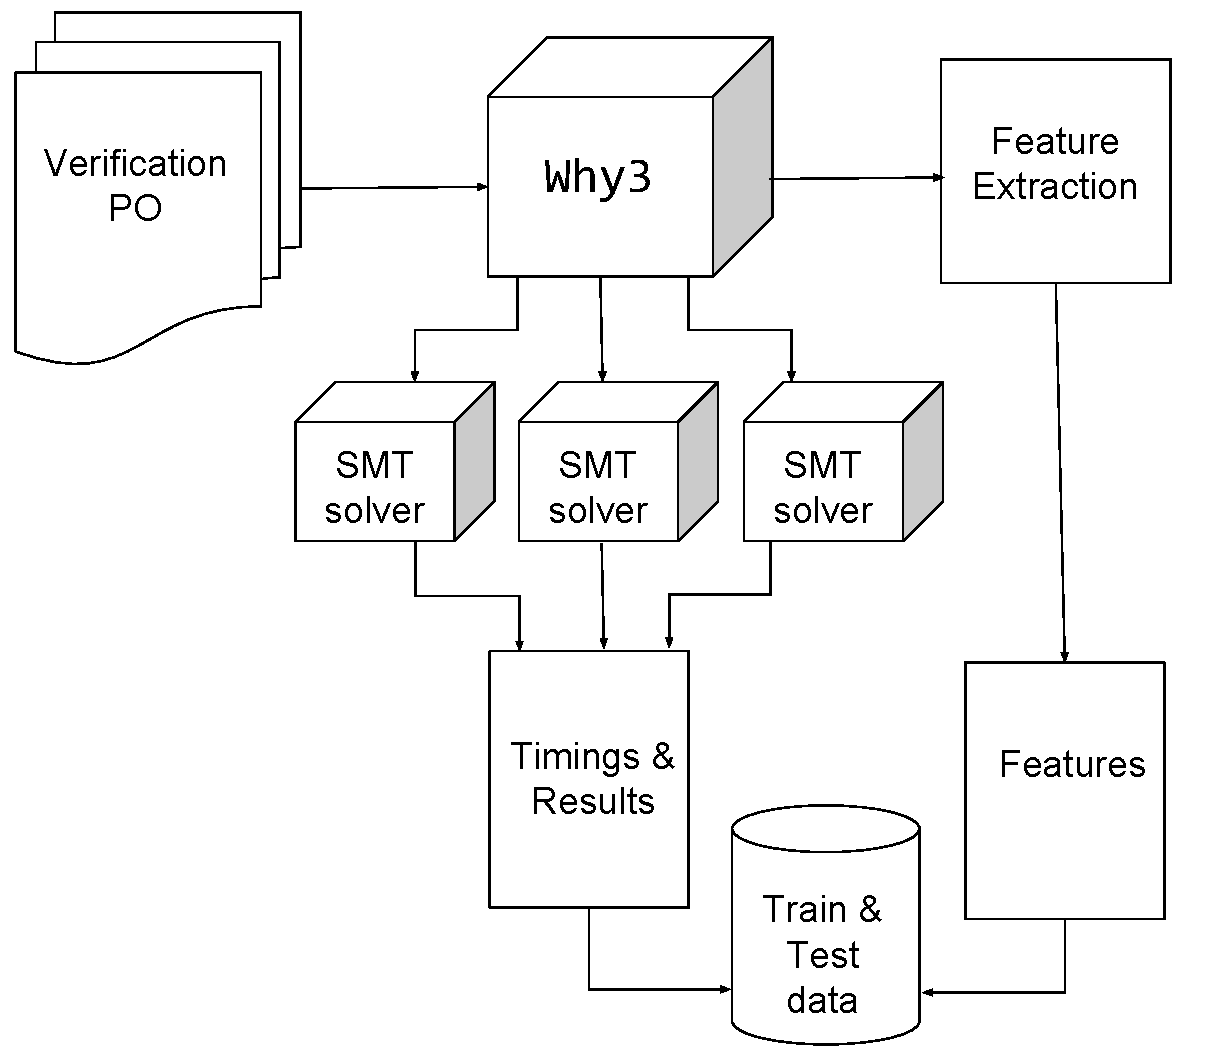
\includegraphics[width=0.9\linewidth]{Figures/Chapter3}
\caption{Diagram illustrating the process to collect predictor and response variables for the \where~model}
\label{fig:Chapter3}
\end{figure}

\section{Selection of tools and programs}
\label{sec:selection}

\subsection{Selection of \why~programs}
\label{sub:why3programs}

As we mentioned in Chapter \ref{LitReview}, \why~was chosen for its modular architecture and ability to read from, and write to, many formats associated with software verification tools. The diversity of input languages in the SV domain was referenced in the previous chapter (Sec. \ref{sub:lrsvmmbench}, \cite{Dagstuhl, deductiveSV}). %Among the input formats which can be parsed by \why are:
%the why intermediate logic format
%
%\begin{itemize}
%	\item \texttt{whyML}: a programming language with support for verification specifications and annotations (native)
%	\item \texttt{why}: the intermediate logic language (native)
%	\item \texttt{TPTP}: the  
%	\item \texttt{Dimacs}: A standard input format for SAT solvers
%\end{itemize} 
We refer the reader to the summary of major benchmark repositories for SV tools given in Table \ref{table:benchmarks}. 
Given the lack of a large standard benchmark repository for software verification systems, we chose to make use of the 128 example programs written in the WhyML programming language as our corpus for training and testing purposes. 
%The programs contain solutions to challenges from the VerifyThis competition and the VACID-0 benchmarks.
These programs are distributed with the \why~software; we used version 0.87.1. 
Many of the programs are solutions to problems posed at software verification competitions such as VerifyThis \cite{verifythis}, VSTTE \cite{Klebanov2011} and COST \cite{bormer:hal-00789525}. 
Other programs are implementations of benchmarks proposed by the VACID-0 \cite{Leino10vacid-0:verification} initiative.   

It is our assumption that the \why~examples are representative of software verification workload. Two alternatives to this dataset are the TPTP \cite{TPTP} library and the BWARE \cite{Delahaye2014} collection of industrial proof obligations. The latter dataset consists of Atelier-B  POs translated into the TPTP format \cite{atelierB2w}. 
The TPTP repository is limited to first-order logic problems: inductive problems cannot be expressed. 
The BWARE SMT-LIB translation uses an upper-bound logic of UFNIA -- this set of theories does not use arrays or real arithmetic\footnote{More information about the SMT-LIB standard for logical theories can be found at \url{http://smtlib.cs.uiowa.edu/logics.shtml} }. 
Both datasets are, however, much larger. The TPTP library currently consists of 20,306 POs \cite{TPTPsite} -- many of which are very similar to each other. There are 12,876 BWARE benchmarks. In comparison, the 128 WhyML programs produced 1048 individual proof obligations. 

The TIP (Tons of Inductive Problems) benchmarks \cite{Claessen2015}, while interesting, were not considered for use as they only measure one aspect of a set of SV tools: their ability to discharge proof obligations which require the use of induction. 

Importantly, the chosen dataset makes use of the full capabilities of the \why~system: the programs include inductive problems and require the use of as many logical theories as each individual SMT solver can reason with.   

\subsection{Selection of \textsc{SMT} solvers}
\label{sub:smtselection}

We used six current, general-purpose SMT solvers supported by \textsf{Why3}: 
\begin{itemize}
	\item \textbf{Alt-Ergo} is a general-purpose SMT solver written in OCaml (the others in this list are written in C++). It is the most tightly-integrated solver supported by \why: it supports polymorphic types and its native input format is a previous version of the \why~intermediate language. Two recent major versions, 0.95.1 and 1.01, are used by \where.
	\item \textbf{CVC3} is the open-source SMT solver developed by the University of Iowa and New York University. We used version 2.4.1.
	\item \textbf{CVC4} is an entirely re-implemented update to CVC3. Version 1.4 is used by \where.
	\item \textbf{veriT} is an open-source SMT solver developed by the University of Lorraine, France, and the Federal University of Rio Grande do Norte, Brazil. We used the current version, 201506, which is not officially supported by \why~v.0.87.1 but is the only version available.
	\item \textbf{Yices} is developed by SRI International and is free for non-commercial use. \where~uses version 1.0.38 rather than Yices2 because the newer implementation does not support quantifiers -- making it unsuitable for SV.  
	\item \textbf{Z3} is the SMT solver developed at Microsoft Research. The source code has been available since 2012 and it has been open-source since 2015. \where~uses two versions: 4.3.2 and 4.4.1. 
\end{itemize}

As Table \ref{table:solvers} shows, the six solvers use four different input formats between them -- three of which are specific to the solver in question. 
This gives some idea of the interoperability capabilities of \why~and the difficulties of comparing tools with a diverse range of input languages. 

Using two versions of Alt-Ergo and Z3 affords the user more flexibility in their local SMT solver installation. 
We describe the process \where~uses to find and use supported SMT solvers on a user's local machine in Chapter~\ref{Implementation}. 

\begin{table}
	\caption[SMT solvers supported by \where]{SMT solvers supported by \where}
 
		\begin{tabularx}{\textwidth}{@{}YYYc@{}}
			\toprule
			\textsc{Solver} &  \textsc{Licence} & \textsc{Why3 driver output} & \textsc{Reference} \\
			%\midrule
			\midrule
			Alt-Ergo & CeCILL-C & \texttt{.why}: Alt-Ergo native input format & \cite{AltErgo} \\ 
			\midrule
			CVC3 & Open-source & \texttt{.cvc}: CVC3 native input format & \cite{CVC3} \\
			\midrule
			CVC4 & BSD & \texttt{.smt}: SMT-LIB version 2 & \cite{CVC4} \\ 
			\midrule
			veriT & BSD & \texttt{.smt}: SMT-LIB version 2 & \cite{veriT} \\
			\midrule
			Yices & Non-commercial use & \texttt{.ycs}: Yices native input format & \cite{Yices} \\
			\midrule
			Z3 & MIT & \texttt{.smt}: SMT-LIB version 2 & \cite{Z3} \\
			\bottomrule	
			
		\end{tabularx}
	
	\label{table:solvers}
\end{table}


\section{Independent/Predictor variables}
\label{sec:independant}

In supervised machine learning terms, these variables represent the known properties of the item from which we want to derive a prediction (in the present case, this item is a computer program). 
The predictor variables must be an accurate characterisation of the program in order for the ML model to be effective. 
We chose to use the proof obligations from goals and lemmas rather than those from axioms and predicates (which tend to be repeated in files using the same logical theories). 
Proof obligations are generated from the goals and lemmas only, while the axioms and predicates provide the context for these POs to be proved by the SMT solver.
%The goals and lemmas are the parts sent to the SMT solver to be proved.   

\subsection{Extracting static metrics from \why~proof obligation formul\ae}
\label{sub:extracting}
%Using the \why notion of "goal shape"

\begin{figure}
	\centering
	\begin{tikzpicture}[
	level 1/.style={sibling distance=30mm},
	edge from parent/.style={->,draw},
	>=latex]
	
	\node[root]{Size}
	child {node[level 2] (c0) {ops}
		child {node[level 2, yshift=10pt] (c1) {divisor}}
		child {node[level 2, yshift=10pt] (c2) {conds}}
	}
	child {node[level 2, yshift=-32pt, xshift=55pt] (c3) {leaves}}
	child {node[level 2, yshift=-32pt, xshift=55pt] (c4) {quants}}
	;
	
	\begin{scope}[every node/.style={level 3}]
	\node [below of = c1, xshift=5pt, yshift=10pt] (c11) {and};
	\node [below of = c11, yshift=10pt] (c12) {or};
	\node [below of = c12, yshift=10pt] (c13) {not};
	\node [below of = c13, yshift=10pt] (c14) {let};
	\node [below of = c14, yshift=10pt] (c15) {as};
	\node [below of = c15, yshift=10pt] (c16) {eps};
	\node [below of = c16, yshift=10pt] (c17) {func};
	
	
	\node [below of = c2, xshift=5pt, yshift=10pt] (c21) {if};
	\node [below of = c21, yshift=10pt] (c22) {iff};
	\node [below of = c22, yshift=10pt] (c23) {imp};
	\node [below of = c23, yshift=10pt] (c24) {case};
	
	
	\node [below of = c3, xshift=5pt, yshift=10pt] (c31) {var};
	\node [below of = c31, yshift=10pt] (c32) {true};
	\node [below of = c32, yshift=10pt] (c33) {false};
	\node [below of = c33, yshift=10pt] (c34) {wild};
	\node [below of = c34, yshift=10pt] (c35) {zero-ar};
	\node [below of = c35, yshift=10pt] (c36) {int};
	\node [below of = c36, yshift=10pt] (c37) {float};
	
	
	\node [below of = c4, xshift=5pt, yshift=10pt] (c41) {forall};
	\node [below of = c41, yshift=10pt] (c42) {exists};
	
	\node [below of = c42](c43) {depth};
	\node [below of = c43](c44) {avg-arity};
	
	\end{scope}
	% lines from each level 1 node to every one of its "children"
	\foreach \value in {1,...,7}
	\draw[->] (c1.195) |- (c1\value.west);
	
	\foreach \value in {1,...,4}
	\draw[->] (c2.195) |- (c2\value.west);
	
	\foreach \value in {1,...,7}
	\draw[->] (c3.195) |- (c3\value.west);
	
	\foreach \value in {1,...,2}
	\draw[->] (c4.195) |- (c4\value.west);
	
	\end{tikzpicture}
	\caption{Tree illustrating the Why syntactic features counted by traversing the AST.}
	\label{fig:types}
\end{figure}

To extract the structural metrics from the logical formul\ae, we traversed the abstract syntax tree (AST) representation. 
We made use of the \why~OCaml API to do this. 
Our approach is similar to the method used internally by \why~to derive a \textit{shape} string from an interactive proof session \cite{why:preserving}. 
The purpose of shape strings in this context is to track changes in the POs and avoid re-proving files unnecessarily. 
The shape acts as a minimal fingerprint representing the structure of the PO formula. 
Instead of producing a string after traversing the AST, our process simply counts the syntactic features of the formula to construct a feature vector.

Fig. \ref{fig:types} lists the predictor variables that were used in our study.  
All of these are (integer-valued) metrics that can be calculated by analysing the \textsf{Why3} goal statement, and are similar to the \textit{Syntax} metadata category for proof obligations written in the TPTP format \cite{TPTP}. 
The metrics we chose to characterise \why~proof obligations are intended to generalise for first-order formul\ae~and other IVLs such as Boogie \cite{Boogie} rather than be specific to \why~syntax.
The metrics' simplicity also makes the ML models more transparent and understandable: metrics derived from multiple complicated interactions of structural features would be hard to reason about and apply to other related contexts where learning would be useful. 

The features shown in pink rectangles in Fig. \ref{fig:types} are counted individually by traversing the AST. 
The rounded blue nodes represent metrics that are the sum of their children in the tree. 
The metrics represented by pink rectangles measure syntactic features and are self-explanatory except for the following:
\begin{itemize}[leftmargin=*]
	\item[] \textbf{zero-ar:} The number of functions which do not take any arguments (i.e. zero-arity functions).
	\item[] \textbf{depth:} The depth of the AST.
	\item[] \textbf{avg-arity:} The total number of arguments for all functions which are children of the \textit{divisor} node, divided by the value of \textit{divisor}.
\end{itemize}   

\textit{Size} measures the size the expression and is the sum of \textit{ops} (the number of operators), \textit{leaves} (the number of leaf nodes in the AST), and \textit{quants} (the number of quantifiers). 
We map our notion of \textit{conds} to the number of decision nodes used to calculate McCabe's cyclomatic complexity metric discussed in Sec. \ref{sec:lrmm}.

Options for the extraction of features from WhyML programs were limited.
The domain specific language makes this process more difficult in comparison to related work which uses the general-purpose C language \cite{DPVZ15:CAV, MUX}.
As a result, we decided to use the purely syntactic analysis outlined in this subsection (along with meta information such as the size of the expression, average arity and depth of AST). 
Keeping the choice of independent variables simple also has the effect of increasing generalisability to other formalisms such as Microsoft's Boogie \cite{Boogie} intermediate language.
A direction for future work disscussed in Chapter \ref{Conclusion} is to investigate more elaborate methods for feature extraction.
   
  

\subsubsection{Example: \textit{first\_last} lemma}

As a minimal illustrative example, we refer to the code listing in Fig. \ref{fig:code}. 
This code is one of the 13 POs from the \texttt{edit\_distance.mlw} file in the \why~examples directory. 
The entire program verifies an algorithm which finds the ``edit distance''\footnote{\url{https://en.wikipedia.org/wiki/Edit_distance}} similarity measure between two strings.  
Informally, this intermediate lemma asserts that the same words are produced by (i) prepending a word (minus its first letter \textit{a}) with \textit{a} and (ii) appending a word (minus its last letter \textit{b}) with \textit{b}. 
A representation of the parse tree from this lemma is shown in Fig. \ref{fig:tree}. 
The root node (\textit{forall}) is circled and the leaf nodes are shown as rectangles.
The name of each \textit{func} (as interpreted by \why) is shown for clarity.
The reader will note that the zero-arity function \textit{Nil} is a leaf node in the tree, while all other functions (\textit{Cons, =, ++, length}) and operators (\textit{and}) have an arity of either 1 or 2. 

Table \ref{table:examplemetrics} shows the non-zero metrics used to describe the \textit{first\_last} formula for predictive purposes.

\begin{figure}
	\centering 
	\lstinputlisting[language=ML, firstline=60, lastline=62]{edit_distance.txt}
	\caption{ \textit{WhyML} code for the \textit{first\_last} lemma in \textit{edit\_distance.mlw}}
	\label{fig:code}
\end{figure}

\begin{figure}
	\centering
	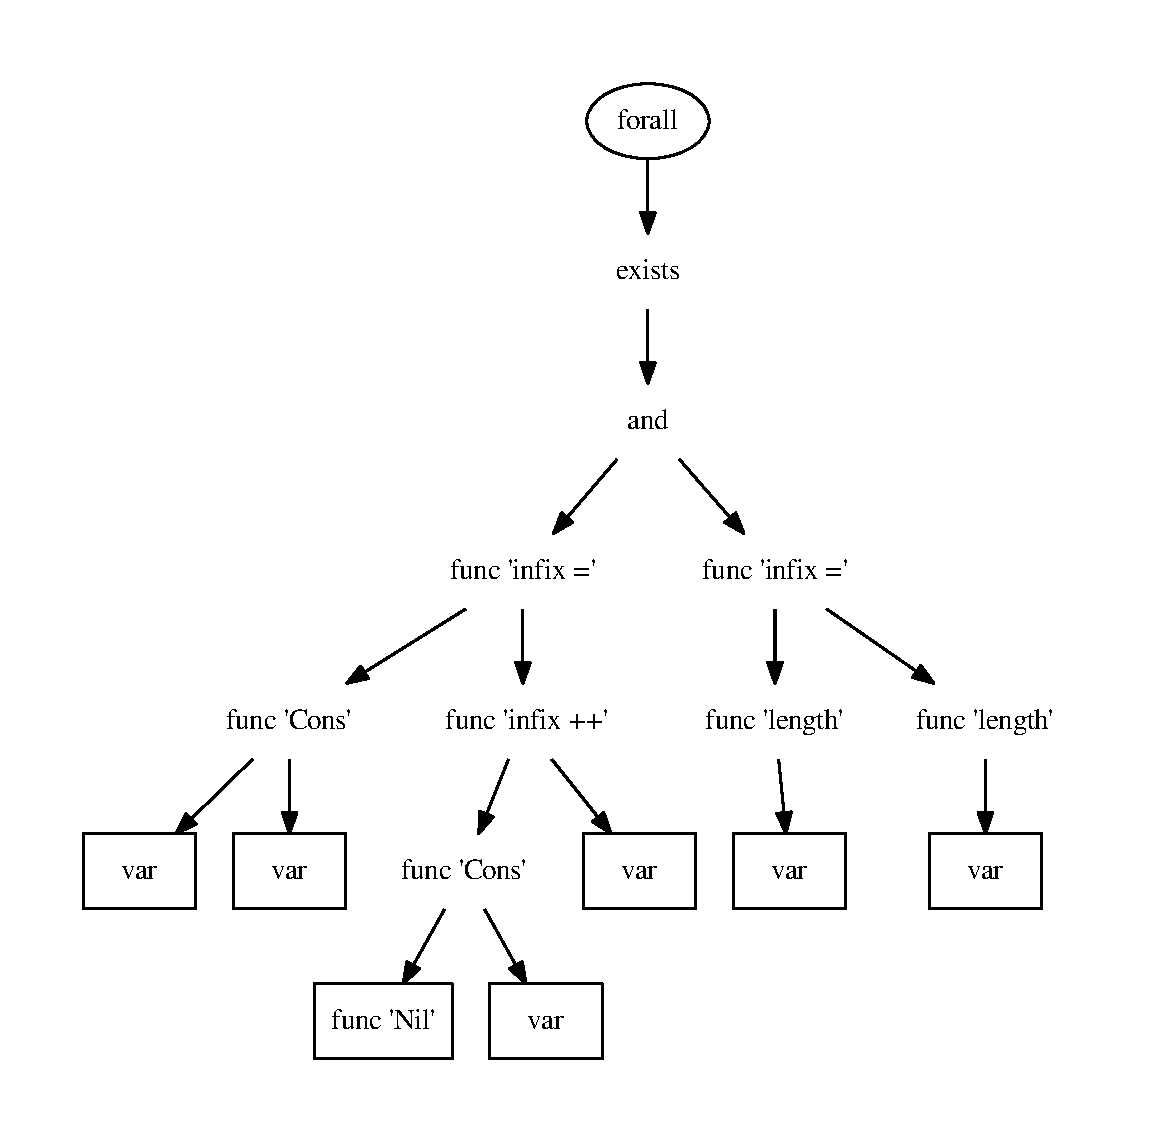
\includegraphics[width=0.9\textwidth]{code}
	\caption{The parse tree extracted from the \textit{first\_last} goal (Fig. \ref{fig:code})}
	\label{fig:tree}
\end{figure}

%%

% 	"and": 1.0,
% 	"exists": 1.0,
% 	"n_quants": 2.0,
% 	"zero_ar": 1.0,
% 	"n_branches": 7.0,
% 	"n_ops": 9.0,
% 	"var": 6.0,
% 	"size": 17.0,
% 	"avg_op_arity": 1.55
% 	"forall": 1.0,
% 	"func": 8.0,
% 	"divisor": 9.0,
% 	"depth": 7.0,

%% 

\begin{table}
	\centering
	\caption{Non-zero metrics calculated for \textit{first\_last}} 
	\label{table:examplemetrics}
	\begin{tabular}
		{|r|r|c|r|r|c|r|r|} \hline
		Metric&Value&&Metric&Value&&Metric&Value \\ \hline
		\texttt{and}&1&&\texttt{exists}&1&&\texttt{forall}&1 \\ \hline
		\texttt{var}&6&&\texttt{func}&8&&\texttt{quants}&2 \\ \hline
		\texttt{ops}&9&&\texttt{leaves}&7&&\texttt{depth}&7 \\ \hline
		\texttt{size}&17&&\texttt{divisor}&9&& \texttt{avg\_arity}&1.55 \\ 
		\hline
		\texttt{zero\_ar}&1&& & && & \\ \hline	
	\end{tabular}
\end{table}


\section{Dependent/Response variables}
%Measurement of dynamic properties
\label{sec:dependant}

Our evaluation of the performance of a solver depends on two factors: the time taken to calculate the result, and the solver's output as interpreted by \why.

\subsection{Execution time}
%mention the rationale behind choosing 10 seconds as a reasonable time limit   
In order to accurately measure the time each solver takes to return an answer, we used a measurement framework specifically designed for use in competitive environments. 
The BenchExec \cite{ Beyer2016,benchexec} framework was developed by the organisers of the SV-COMP \cite{SVCOMP} software verification competition to reliably measure CPU time, wall-clock time and memory usage of software verification tools. 
We recorded the time spent on CPU by each SMT solver for each proof obligation. 

\subsubsection{Accounting for randomness with confidence intervals}
\label{sub:confidence}

Any effort to measure execution time accurately is hampered by random errors introduced by the experimental environment.
Such errors are inherent to measuring time in real world computing environments due to factors such as cache misses, competing processes and instructions needed to perform the measurement itself.   
These errors affect the \textit{precision} of the experiment: ie. how likely a result is to be repeated \textit{exactly} across multiple experiments. 
To account for these errors, we used the methodology described by Lilja \cite{LiljaJ} to obtain the number of measurements needed to make an approximation of the true mean execution time. 

As each solver execution can be quite expensive in terms of time (a worst case scenario for one measurement of each PO: 1048 (POs) $\times$ eight (solvers) $\times$ ten seconds (time limit) $\approxeq$ 23.3 hours of computation time), a small number of initial measurements (five) were made. 
From these sample measurements, the mean execution time $\bar{x}$ and standard deviation $s$ were computed. 

To determine the number of measurements ($n$) required for a statistically-significant sample, Lilja recommends that we assume the random errors have a $Student's$ $t$-distribution (similar in shape -- although more spread out -- to a Gaussian distribution). 
An assumption of the error's distribution is required as there is no \textit{reference value} (ie. the absolutely \textit{correct} time taken by the solver to execute) available.
This distribution is chosen as the number of sample measurements taken ($<30$) is small whereas if it was large, we could assume errors follow a Gaussian distribution.
When comparing the two distributions, differing results are most obvious when we use a very small ($<4$) degree of freedom to determine the confidence interval (ie. measurements at the higher and lower end of the range are given more importance). 
As the following example using seven degrees of freedom shows, this effect is not applicable to our methodology.  

We use the five measurements to find the confidence interval $(c_1, c_2)$ using the equations:
\begin{equation}
	c_1=(1-e)\bar{x} = \bar{x}-z_{1-a/2;n-1}\frac{s}{\sqrt{n}} 
	\label{eq:c1}
\end{equation}
\begin{equation}
	c_2=(1+e)\bar{x} = \bar{x}+z_{1-a/2;n-1}\frac{s}{\sqrt{n}}
	\label{eq:c2}
\end{equation}
Either Equation \ref{eq:c1} or \ref{eq:c2} can be used to find 
\begin{equation}
	z_{1-a/2}\frac{s}{\sqrt{n}} = \bar{x}e.
	\label{eq:simp}
\end{equation}
Solving for $n$ gives
\begin{equation}
	n =
	 \left(\frac{z_{1-a/2}s}{e\bar{x}}\right)^2
	\label{eq:n}
\end{equation}
  
where $z$ is a value from the $t$-distribution which is used to model the measurement error. 
An illustration of this distribution, Fig. \ref{fig:confidence}, shows that there is a probability $1-a$ that the actual value being measured (i.e. \textit{x}: the execution time for each solver to return an answer for a particular PO), is within the confidence interval ($c_1, c_2$). 
As the bounds of ($c_1, c_2$) increase outward, the confidence level increases.
We can be 100\% confident that the actual mean value is within the interval (0, $\infty$) but this interval is not practical.  
A value of 0.1 was chosen for \textit{a}, meaning we can be 90\% confident that the actual value of \textit{x} is between $c_1$ and $c_2$. 
We allow the computed mean value to be within 7\% of the actual mean (i.e. seven degrees of freedom or an allowed error of $\pm$3.5\%). Thus for the equations \ref{eq:c1} to \ref{eq:n}, we take $e = 0.035$.  \\ 
\\
\textbf{Example: finding Alt-Ergo's execution time for \textit{first\_last}}: \\
To show how this method is used in practice, we return to the example introduced in Sec. \ref{sub:extracting} -- the \textit{first\_last} goal from \textbf{edit\_distance.mlw}'s \textbf{Word} theory.
The five sample measurements of CPU time spent by Alt-Ergo (to return an answer of \textit{Unknown}):

\begin{tabularx}
	{\textwidth}{@{}YYYYY@{}}
	 $\lbrace$ 0.124, & 0.142, & 0.136, & 0.131, & 0.133 $\rbrace$
\end{tabularx} 

given a sample mean ($\bar{x}$) and sample standard deviation ($s$) of 0.133 and 0.006 respectively. 
Consulting a table for the $t$ distribution, we find that when $a=0.1$ and we require seven degrees of freedom, $t_{0.95;7} = 1.895$.
Substituting these values into equation \ref{eq:n}, we find
\begin{equation}
	n =  \left(\frac{z_{1-a/2}s}{e\bar{x}}\right)^2
	= \left(\frac{1.895(0.006)}{0.035(0.133)}\right)^2 = 5.966
\end{equation}    
Therefore, we need to make six measurements to be assured that there is a 90\% chance that the true value is within this $\pm3.5\%$ interval.

For completeness, the extra measurement yielded a value of 0.135; making the CPU time Alt-Ergo spent solving \textit{first\_last} the mean of the six measurements: 0.134 seconds.

\begin{figure}
\centering
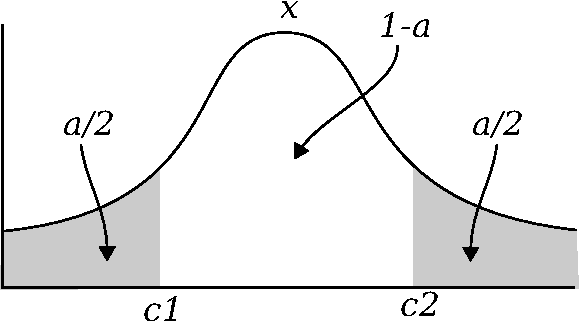
\includegraphics[width=0.6\linewidth]{Figures/confidence}
\caption[Accounting for errors in measurement of solver execution time \textit{x}]{Accounting for errors in measurement of solver execution time \textit{x}}
\label{fig:confidence}
\end{figure}


%By inspecting our data, we saw that most \textit{Valid} and \textit{Invalid} answers returned very quickly, with \textit{Unknown} answers taking slightly longer, and \textit{Failure/Timeout} responses taking longest. We took the relative utility of responses to be $Valid >$ $Invalid>Unknown>Timeout>Failure$ which can be read as ``it is better for a solver to return a \textit{Valid} response than \textit{Timeout}'', etc. A simple function allocates a cost to each solver $S$'s response to each goal $G$:
%\[\small
%cost(S,G) = 
%\begin{cases}
%time_{S,G}, \text{ if answer}_{S,G} \in \lbrace Valid, Invalid \rbrace \\
%time_{S,G} + \text{timeout}, \text{ if answer}_{S,G} = Unknown \\
%dist((time_{S,G},\text{timeout}), (0,0)), \text{if answer}_{S,G} \in \lbrace Timeout, Failure \rbrace
%\end{cases}
%\]
%
%Thus, to penalise the solvers that return an \textit{Unknown} result, the timeout limit is added to the time taken, while solvers returning \textit{Timeout} or \textit{Failure} are further penalised by taking the Euclidean distance from $(0,0)$ to the point defined by the (time taken, timeout limit). This function ensures the best-performing solvers always have the lowest costs. A ranking of solvers for each goal in order of decreasing relevance is obtained by sorting the solvers by ascending cost.
%
%Since our cost model depends on the timeout value chosen, we need to choose a value that does not favour any one solver.  To establish a realistic timeout limit, we find each solver's ``Peter Principle Point'' \cite{Sutcliffe200139}. In resource allocation for theorem proving terms, this point can be defined as the time limit at which more resources will not lead to a significant increase in the number of goals the solver can prove. 

\subsection{Prover output}
\label{sub:prover-output}

\begin{figure}
	\centering
	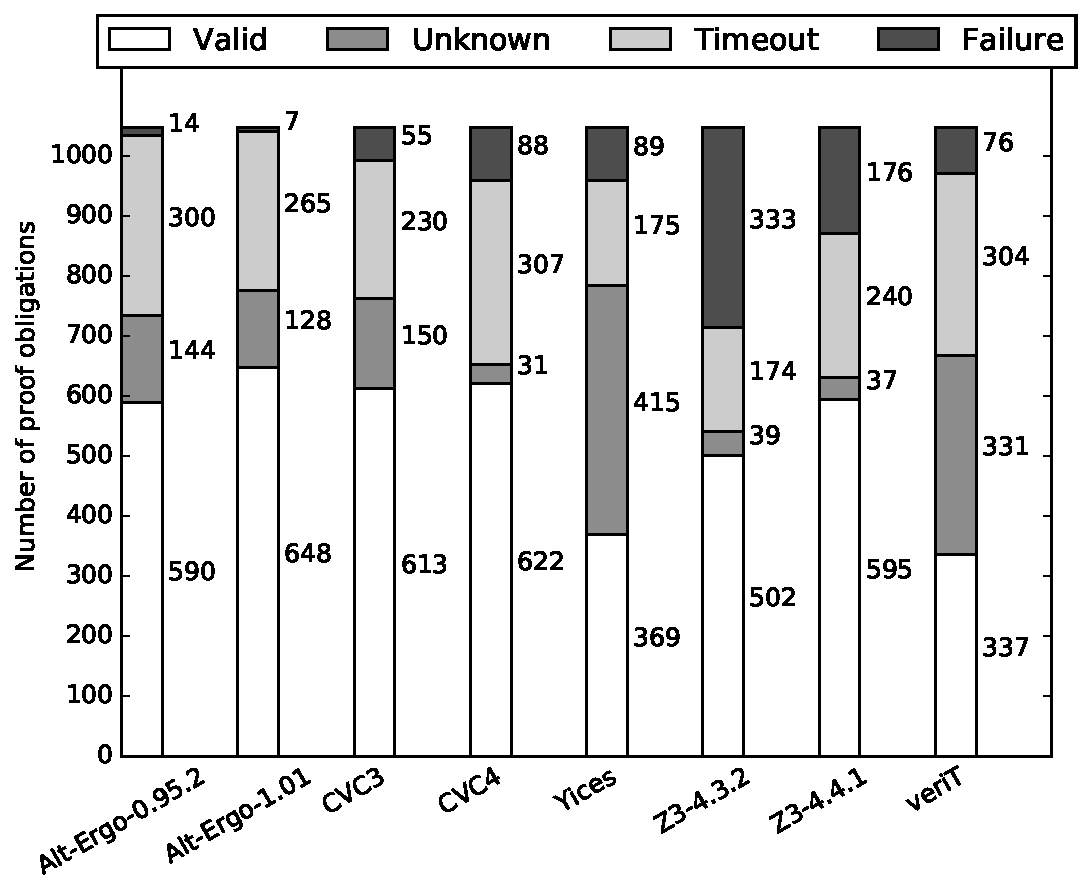
\includegraphics[width=0.8\linewidth]{barcharts}
	\caption[The relative amount of Valid / Unknown / Timeout / Failure answers from the eight SMT solvers]{The relative amount of Valid / Unknown / Timeout / Failure answers from the eight SMT solvers (with a timeout of 60 seconds). }
	\label{fig:barcharts}
\end{figure}


When a solver is sent a goal by \why, it returns an answer $A$ where $A$ is one of $\lbrace Valid,Invalid,Unknown,Timeout,Failure \rbrace$. The following definitions of these answers are taken from the \why~User Manual \cite{why:manual}.\\  

\begin{tabularx}
	{\textwidth}{@{}ll@{}}
	\textbf{Valid}   & The goal is proved in the given context. \\
	\textbf{Invalid} & The prover knows the goal cannot be proved. \\  
	\textbf{Unknown} & The prover has stopped its search.\\
	\textbf{Timeout} & The prover has reached the time limit. \\
	\textbf{Failure} & An error has occurred. \\
\end{tabularx}\\

Fig. \ref{fig:barcharts} shows the relative amount of $Valid / Unknown / Timeout / Failure$ answers from the eight SMT solvers (when given a timeout of 60 seconds) on the entire dataset of 1048 POs. 
For example, Alt-Ergo version 0.95.1 (leftmost bar) returned an answer of \textit{Valid} for 590 POs, \textit{Unknown} for 144 POs, \textit{Timeout} for 300, and \textit{Failure} for 14.
Note that no tool returned an answer of Invalid for any of the 1048 proof obligations.
We assume this is because the example programs are verified algorithms/data-structures and an answer of \textit{Invalid} would indicate a violated pre-/post- condition or invariant.
The limitations of our chosen dataset and other threats to validity are discussed later in the thesis (Sec. \ref{sec:threats}).

Often, goals that cannot be proved \textit{Valid} or \textit{Invalid} require inductive reasoning through the use of an interactive theorem prover such as Isabelle \cite{Isabelle} or Coq \cite{Coq}. 
Sometimes a splitting transformation needs to be applied in order to simplify the goals before they are sent to the solver. 
\where~does not perform any transformations to goals other than those defined by the solver's \why~driver file. 
In other cases, more time or memory resources need to be allocated in order to return a conclusive result. 
We address the issue of resource allocation in the next subsection.    

\subsubsection{Setting a timeout limit for measurement}
\label{sub:timeout-limit}

\begin{figure}
	\centering
	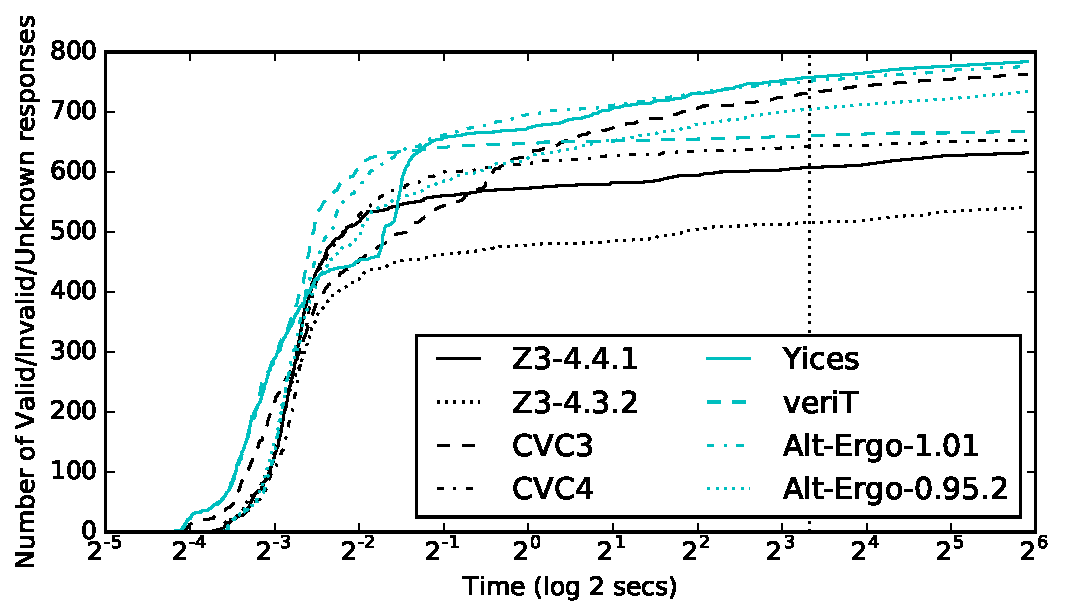
\includegraphics[width=\linewidth]{line_graph}
	\caption[Cumulative number of useful responses for each solver over 60 seconds]{The cumulative number of \textit{Valid/Invalid/Unknown} responses for each solver for the entire dataset of 1048 POs. The plot uses a logarithmic scale on the time axis for increased clarity at the low end of the scale.}
	\label{fig:line_graph}
\end{figure}

\sloppypar
A solver is said to return a \textit{useful} result if it returns an answer of \textit{Valid}, \textit{Invalid} or \textit{Unknown} when given a reasonable timeout limit.
We justify this statement by making the observation that an answer of \textit{Failure} usually means there is an error in logical translation of the PO. 
The failing solver is not a good choice for the particular logics required to return a \textit{Valid} or \textit{Invalid} answer.
\textit{Unknown} answers are usually identified as such very quickly therefore they do not impose a long waiting period for an answer and \where~can call another solver with a minimal delay.
By definition, \textit{Timeout} results incur the maximal time penalty.  
    
Fig. \ref{fig:line_graph} shows the number of \textit{Valid/Invalid/Unknown} results for each solver when given a timeout value of 60 seconds. 
For example, the solid black line shows the useful results for version 4.4.1 of Z3.
At $2^{-3}$ (0.125) seconds, Z3 returned 130 \textit{Valid/Invalid/Unknown} results. 
This number increases sharply to 518 after $2^{-2}$ (0.25) seconds, before levelling off.
If Z3 is given a time limit of 60 seconds, only 125 more useful responses are returned; giving a total of 632.  

The value of 60 seconds was chosen as an upper limit, since this timeout value is not realistic for most software verification scenarios.  
\why, for example, has a default timeout value of five seconds.
By inspecting the plot of solver answers in Fig. \ref{fig:line_graph}, we can see that the number of useful answers returned levels off very quickly. 
From this observation we deduce that the likelihood of a \textit{Timeout} answer potentially turning into a \textit{Valid/Invalid} answer (if given more time) is minimal.  
%From Fig. \ref{fig:line_graph} we can see that the vast majority of useful responses are returned very quickly. 

To establish a realistic timeout limit, we find each solver's ``Peter Principle Point'' \cite{Sutcliffe200139}. In resource allocation for theorem proving terms, this point can be defined as the time limit at which more resources will not lead to a significant increase in the number of goals the solver can prove.
By satisfying ourselves with being able to record 99\% of the useful responses which would be returned after 60 seconds, a more reasonable threshold is obtained for each solver. 
To calculate this time value for each solver, we find the time at which 99\% of the solver's total number of \textit{Valid / Invalid / Unknown} responses have be returned. 
This threshold ranges from 7.35 secs (veriT) to 9.69 secs (Z3-4.3.2). Thus we chose a value of ten seconds (Fig. \ref{fig:line_graph}'s \textit{dotted vertical line}) as a representative, realistic timeout that gives each solver a fair opportunity to return decent results.     



\section{Summary}

In this chapter, we have introduced the SMT solvers, training and testing dataset, predictor and response variables used by the \where~model.
The choices made in regard to the SMT solvers were dictated to a large extent by \why~and its selection of drivers. 
The dataset contains solutions to canonical SV challenges and is designed to demonstrate the specification and verification of data structures and algorithms fundamental to a wide range of applications, using the full capabilities of the \why~system.
The choice of predictor variables was influenced by the structural metrics introduced by McCabe (see Sec. \ref{sec:lrmm}), which have become established in the SE domain, and syntactic features similar to those used in TPTP library metadata. 
The response variables of \textit{time} and \textit{result} are similar to the scoring mechanism used for SV tools in the SV-COMP \cite{SVCOMP}.
The response variables will be combined in the next chapter as a single value suitable for prediction by a variety of regression models.

After conducting the data preparation discussed in this chapter, we have collected particular information about each proof obligation: 
\begin{itemize}
	\item the time each of the eight solvers takes to return an answer when given a time limit value of ten seconds
	\item each solver's response (\textit{Valid/Timeout/etc.}) for the same time limit
	\item a feature vector consisting of the twenty-eight structural and syntactic metrics listed in Fig. \ref{fig:types} 
\end{itemize}   
The material presented in this chapter is critical to how the \where~model functions and forms the basis for the experiments presented in the next chapter. 
  



\chapter{Choosing a Prediction Model}
\thispagestyle{nohead}
\label{Prediction}

This chapter will evaluate the effectiveness of a number of machine learning algorithms at predicting the most appropriate SMT solver to use on any (unseen) \textsf{Why3} PO.
Our goal in this thesis is to construct a ``meta-solver'' or \textit{portfolio} solver which chooses from a range of tools in order to prove more goals than a single solver is capable of.
We motivate the need for a portfolio solver with an analysis of our dataset 
in Sec. \ref{sec:portfolio-benefit}. 
More details about the type of prediction task chosen for the evaluation of ML algorithms is given in Sec. \ref{sec:reg-class}.
A more detailed introduction to the six prediction algorithms (some of which were introduced previously in Sec. \ref{sec:lrml} and Table \ref{table:algorithms}) is given in Sec. \ref{pred:choosing} before the results of their comparison is discussed. 
We make this comparison with reference to a number of theoretical strategies introduced in Sec. \ref{sec:strategies}.
We end this chapter with a more detailed look at the model chosen for use in the actual implementation of \where.

Throughout this chapter, we use the terms ``algorithms'' and ``models'' to refer to different, but related, concepts. An ``algorithm'' refers to the general approach to prediction, as formalised to be applicable to a number of prediction scenarios.
``Models'' are trained instances of these algorithms which use specific parameters and data to make predictions for a single use case.

\section{The benefit of portfolio-solving in \why}
\label{sec:portfolio-benefit}

\newcolumntype{Z}{>{\raggedleft\arraybackslash}X} 
\begin{table}
	\caption[Results of running eight solvers on the example \textsf{Why3} programs]{Results of running eight solvers on the example \textsf{Why3} programs.  Also included is a theoretical solver  \textsf{Choose Single}, which always returns the best answer in the fastest time.}
	\begin{tabularx}{1.1\textwidth}{@{}l|ZZZ|ZZZ|ZZZ@{}}
		\toprule
		{} & \multicolumn{3}{c|}{\textbf{File}} & \multicolumn{3}{c|}{\textbf{Theory}} & \multicolumn{3}{c}{\textbf{Goal}} \\
		{} & \# proved & \% proved & Avg time & \# proved & \% proved & Avg time & \# proved & \% proved & Avg time \\
		\midrule
		\textsf{Choose Single} & \textbf{48} & \textbf{37.5\%} & \textbf{1.90} & \textbf{190} & \textbf{63.8\%} & \textbf{1.03} & \textbf{837} & \textbf{79.9\%} & \textbf{0.42} \\
		\textbf{Alt-Ergo-0.95.2} & 25 & 19.5\% & 1.45 & 118 & 39.6\%& 0.77 & 568 & 54.2\% & 0.54 \\ 
		\textbf{Alt-Ergo-1.01} & 34 & 26.6\% & 1.70 & 142 & 47.7\% & 0.79 & 632 & 60.3\% & 0.48 \\ 
		\textbf{CVC3} & 19 & 14.8\% & 1.06 & 128 & 43.0\% & 0.65 & 597 & 57.0\% & 0.49 \\ 
		\textbf{CVC4} & 19  & 14.8\% & 1.09 & 117 & 39.3\% & 0.51 & 612 & 58.4\% & 0.37 \\ 
		\textbf{veriT} & 5 & 4.0\% & 0.12 & 79 & 26.5\% & 0.20 & 333 & 31.8\% & 0.26 \\ 
		\textbf{Yices} & 14 & 10.9\% & 0.53 & 102 & 34.2\% & 0.22 & 368 & 35.1\% & 0.22 \\ 
		\textbf{Z3-4.3.2} & 25 & 19.5\% & 0.56 & 128 & 43.0\% & 0.36 & 488 & 46.6\% & 0.38 \\ 
		\textbf{Z3-4.4.1} & 26 & 20.3\% & 0.58 & 130 & 43.6\% & 0.40 & 581 & 55.4\% & 0.35 \\ 
		\bottomrule
	\end{tabularx}
	\label{table:avgtimes}
\end{table} 
%
%\begin{table}
%	\centering
%	\caption[Number of trivial and hard \textsf{Why3}verification tasks]{Number of trivial and hard \textsf{Why3}verification tasks}
%	\begin{tabularx}{0.8\textwidth}{@{}l|ZZZ@{}}
%		{} & \multicolumn{1}{r}{\textbf{File}} & \multicolumn{1}{r}{\textbf{Theory}} & \multicolumn{1}{r}{\textbf{Goal}} \\	
%		\midrule
%		\textbf{Trivial} (all solvers can prove) & 3 & 55 & 206 \\
%		\textbf{Hard} (no solver can prove) & 85 & 118 & 211 \\
%	\end{tabularx}
%	\label{table:trivial-hard}
%\end{table} 

\begin{table}
	\centering
	\caption[Breakdown of results in terms of triviality and hardness]{Breakdown of results in terms of triviality and hardness}
	\begin{tabularx}{0.9\textwidth}{@{}l|ZZZ@{}}
		{} & \multicolumn{1}{r}{\textbf{File}} & \multicolumn{1}{r}{\textbf{Theory}} & \multicolumn{1}{r}{\textbf{Goal}} \\	
		\midrule
		
		\textbf{Trivial} (all solvers can prove) & 3 & 55 & 206 \\
		\textbf{Hard} (no solver can prove) & 85 & 118 & 211 \\
		\midrule
		\multicolumn{4}{c}{\textsc{Uniquely-provable by a single solver}} \\
		\midrule
		\textbf{Alt-Ergo-0.95.2} & 0 & 0 & 1 \\ 
		\textbf{Alt-Ergo-1.01} & 6 & 12 & 25 \\ 
		\textbf{CVC3} & 2 & 3 & 17 \\ 
		\textbf{CVC4} & 1 & 6 & 33 \\ 
		\textbf{veriT} & 0 & 0 & 0 \\ 
		\textbf{Yices} & 0 & 0 & 2 \\ 
		\textbf{Z3-4.3.2} & 0 & 0 & 0 \\ 
		\textbf{Z3-4.4.1} & 0 & 0 & 2 \\ 
		\midrule
		\textbf{Others}: provable by at least two, & 32 & 104 & 551 \\
		but not all, solvers & & & \\
		\midrule
		\textsc{total} & 129 & 298 & 1048 \\
		\bottomrule
	\end{tabularx}
	\label{table:unique}
\end{table} 


Now that the SMT solvers to be supported by \textsf{Where4} have been identified and an appropriate dataset for training and testing purposes has been chosen, we can make a preliminary and exploratory analysis of the behaviour of the SMT tools on the particular data. 
We aim to make a case for portfolio-solving as an effective method for discharging POs in the \textsf{Why3} system.

We refer the reader to Table \ref{table:avgtimes} which shows the results of running eight solvers on the example \textsf{Why3} programs with a timeout value of ten seconds. 
The entire dataset is used in this case. 
WhyML files are modularised as one or more complete \textit{theories} which can be used locally by other theories in the same file. 
The \textsf{Why3} IVL identifies the \textit{goals} which need to be proven in order for the theory (and in turn the entire file) to be verified as correct.
WhyML theories containing assertions and lemmas can produce many goals while others which merely define types and helper functions can produce none. 
Our dataset of 128 WhyML files consists of 289 theories, which in turn generate 1048 goals. 
Aside from the number of each modular construct proved by the solver (\textit{left sub-column}), the percentage this number represents of the total is given (\textit{centre sub-column}) and the average time taken (in seconds) to prove each construct (as measured using the process described in Sec. \ref{sub:confidence}) is given in the \textit{right sub-column}. 

We show the results of proving a WhyML file using its modular constructs. 
This method of verification is particularly useful when \textsf{Why3} is run in batch mode from the command line.
%It is more natural to select separate solvers on a per-goal basis through the \textsf{Why3}IDE which breaks each WhyML program into theories and goals automatically. 
When using the \textsf{Why3} IDE, it is more natural to prove programs by applying solvers to individual goals.
This is because the environment separates WhyML programs into theories and goals automatically.

Table \ref{table:avgtimes} also shows the results for a theoretical solver \textsf{Choose Single}. 
\textsf{Choose Single} is the best solver, from the eight SMT solvers measured, chosen on a per-goal basis. 
For example, if a file contains one theory which consists of three goals, and the best-performing solver is CVC4 for the first goal, Yices for the second, and CVC3 for the third, the result for \textsf{Choose Single} on that file is the sum of the results for CVC4 on the first goal, Yices on the second, etc.
We define what is means for a solver to be the \textit{best} in the next subsection.

The theoretical solver \textsf{Choose Single} shows the benefit of being able to use the most appropriate solver for each PO: 205 more goals are provable -- an increase of 19.6\% -- over the best single solver (Alt-Ergo version 1.01) which can prove a total of 632. 
In total, 837 goals are provable by using a combination of the eight solvers -- a figure that represents 79.9\% of the 1048 goals. 
On average, \textsf{Choose Single} proves goals in a shorter amount of time than either version of Alt-Ergo or CVC3. 
The average time subcolumn provides an insight into how solvers which can prove relatively few goals, theories, or entire files -- such as veriT or Yices -- can be useful in a portfolio-solving context: such solvers often prove what they can in a very short amount of time (veriT takes an average time of just 0.12 seconds, for example, to prove each of five entire files) and can be the best choice of solver for those files, theories and goals. 

The advantages of using multiple solvers are further illustrated by the results presented in Table \ref{table:unique}. \textit{Trivial} files, theories and goals (the first row of Table \ref{table:unique}) are defined as those which can be proved by all eight solvers measured. 
Three files, 55 theories and 206 goals fall under the trivial category.
Again, this table provides an interesting insight into the behaviour of all solvers: three of the five files proved by veriT are trivially provable by all solvers (which may explain the short amount of time taken, on average, to prove the five files). 
The second row of this table shows the number of \textit{hard} files, theories and goals. 
These are the tasks which no solver is able to prove entirely.
As we have previously discussed in Sec. \ref{sub:prover-output}, these goals usually require the use of an ITP or splitting transformation to be discharged.
Two hundred and eleven goals fall under this category.

The breakdown of the number of files, theories and goals which \textit{only one} solver is able to prove is given in Table \ref{table:unique}.
The good performance of Alt-Ergo version 1.01 is obvious: six complete files can only be proved in their entirety by the solver. 
A higher number of goals require the use of CVC4 in order to be proved, however.
Thirty-three goals (compared to twenty-five for the newer version of Alt-Ergo) can \textit{only} be proved by this solver.
The relatively low numbers for files, theories and goals provable by a single solver suggests that most goals can be proved by more than one tool, if they can be proved at all.
Indeed, the second-to-bottom row of Table \ref{table:unique} shows that the majority of goals fall in this category. 

\subsection{The relative utility of solver responses}
\label{sub:rel-util}

To make assertions about the relative performance of different solvers on the same goal, a definition of the relative \textit{utility} of solver responses is required.
Should a solver which returns an answer of \textit{Valid} in five seconds be seen as ``worse'' than one that returns \textit{Unknown} in half a second? 
Likewise, should the solver returning \textit{Failure} after one second be penalised more severely than one returning \textit{Timeout} after the maximum time limit?

We define an ordering for response utility as 
\[
\lbrace Valid, Invalid\rbrace > Unknown > \lbrace Timeout, Failure\rbrace
\]  
the reasoning being that a \textit{Failure} response usually signals a fatal error in the logic encoding for that solver/goal pair, and the learning algorithm should be discouraged from choosing a failing solver for the particular goal characteristics in question. 
As discussed in Sec. \ref{sub:timeout-limit} of the previous chapter, \textit{Unknown} answers are returned quickly in general, and should not be penalised as much as \textit{Timeout} responses. 
Solvers which reach the timeout limit are unlikely to return a \textit{Valid} or \textit{Invalid} response if given more time (illustrated clearly by Fig. \ref{fig:line_graph}).
Solvers returning the same answer are ranked according to runtime -- with faster solvers being preferred.

This method for defining relative performance has similarities to the scoring structure for ATPs competing in SV-COMP \cite{Beyer2016, SVCOMP}, with some important differences. 
In SV-COMP, \textit{Unknown} responses are given a neutral score of 0, the correct reporting of a property which does not hold (``true negative") is rewarded with smaller score ($+1$) than the correct reporting of a property which is found to hold (``true positive" which scores $+2$).
Likewise, the incorrect reporting of a property which does not hold (``false negative" or ``false alarm") is punished less severely (with a score of $-4$) than the incorrect reporting of a property which does hold (``false positives" score $-8$).  
Although the notion of ``false positive'' and ``false negative'' responses is not applicable in the SMT domain (where tools are assumed to be sound), we follow the SV-COMP scoring scheme by warding a ``true positive'' (or \textit{Valid} response) a higher score than a ``true negative'' (or \textit{Invalid} response). 
\textit{Unknown, Timeout} and \textit{Failure} responses are not treated separately by the SV-COMP scoring scheme -- they all fall under the \textit{Unknown} response category.
We penalise poorly-performing solvers through the use of a \textit{cost} function.
%A further refinement to our scoring model was necessary in order for the prediction models to operate effectively. 
The definition of the cost function we applied to solver results is given in Sec. \ref{sub:scoring} of this chapter. 

\section{Classification and regression}
\label{sec:reg-class}

Machine learning prediction tasks can be separated into two categories: those involving the \textit{classification} of a variable into discrete categories or classes, and those predicting a continuous-valued variable directly -- \textit{regression} tasks.
This section will discuss some of the options considered when designing \where's prediction task.

\subsection{Predicting the single best solver} This option involves a multi-class classification task: the classes involved are the eight SMT solvers.
Each PO is classified as belonging in one class. 
We reject this approach because some benefits associated with portfolio-solving are lost, since if the PO is misclassified, the performance of the portfolio solver suffers severely.
For example, the single solver can return an answer of \textit{Failure} with no other solver suggestion being made.
In the best case, the predictions would be equivalent to the \textsf{Choose Single} theoretical solver.

%this method was found to be only marginally better than choosing one of the eight solvers at random. 
\subsection{Predicting the best \textit{ranking} of solvers} Again, this option is a multi-class classification task. 
Instead of predicting a single solver, however, the task involves predicting the entire ranking of eight solvers. 
The benefit of obtaining a ranking is the flexibility it affords in calling SMT solvers sequentially or in parallel.
If the first solver fails or returns an answer other than \textit{Valid} or \textit{Invalid}, the next best predicted solver is called, and so on.

With eight SMT solvers there are eight factorial (or 40,320) rankings which is far too many to be reasonable for a classification task. 
We rejected this approach because in our dataset of 1048 POs many of these rankings could not possibly be represented.
In fact, only 766 of the 40,320 rankings occur in our dataset.  
%Many of these rankings were observed very rarely or did not appear at all in the training data. 
Such an unbalanced representation of classes cannot lead to accurate classification.
\subsection{Predicting solver runtime and response separately}
This approach involves two separate tasks, each predicting a characteristic of the solver's performance. 
One model would attempt to predict the response class (i.e. \textit{Valid, Invalid}, etc.) while another would attempt to predict the solver runtime.
The former task is a multi-class classification task with five classes, while the latter is a multi-output regression task.
This method has the advantage of affording the user flexibility in how to choose the ultimate ranking: for example, if fast responses are preferred over \textit{Valid} answers.
This flexibility comes at the price of complexity, however: two accurate predictors, a classifier and regressor, are required instead of one.
\subsection{Combining the prediction of solver response and runtime}
This option uses a cost function to combine the two solver response variables as a single real-valued number which is used for ranking the solvers.
This is a multi-output regression task: a cost prediction is made for each solver individually.
The individual predicted values are sorted in increasing order to produce a ranking of decreasing ``solver utility''.

This approach shares most of the advantages of predicting solver response and runtime separately: each solver's actual behaviour is predicted directly rather than relying on the relative behaviour of all eight \textit{together} constituting a single class. 
It is relatively simple to change the cost function, although it can not be done ``on-the-fly'' in the same manner as the previous approach allows.
A change to the cost function requires re-training the model.
The major benefit is having one single model to predict both the solver response and the runtime. 
This is the prediction approach chosen for \textsf{Where4} in this thesis.  

\subsection{The Cost Function}
\label{sub:scoring}

The use of a cost function is inspired by the first version of the SATZilla portfolio solver \cite{Satzilla}. 
The cited paper describes the prediction of a \textit{performance score}.
This differs from most portfolio approaches which aim to predict a solver's runtime directly. 

The cost function should reflect the ordering of solver utility defined in Sec. \ref{sub:rel-util}: penalising poorly-performing solvers while ensuring \textit{Valid} and \textit{Invalid} responses incur the lowest cost.
The following simple function allocates a cost to each solver $S$'s response $\langle answer, time\rangle$ to each goal $G$:
\[\small
cost(S,G) = 
\begin{cases}
time_{S,G}, \text{ if answer}_{S,G} \in \lbrace Valid, Invalid \rbrace \\
time_{S,G} + \text{timeout}, \text{ if answer}_{S,G} = Unknown \\
time_{S,G} + (\text{timeout} \times 2), \text{ if answer}_{S,G} \in \lbrace Timeout, Failure \rbrace
%dist((time_{S,G},\text{timeout}), (0,0)), \text{if answer}_{S,G} \in \lbrace Timeout, Failure \rbrace
\end{cases}
\]
Thus, to penalise the solvers that return an \textit{Unknown} result, the timeout limit is added to the time taken, while solvers returning \textit{Timeout} or \textit{Failure} are further penalised by 
adding double the timeout limit to the time taken.
A response of \textit{Failure} refers to an error with the back-end solver and usually means a required logical theory is not supported. 
This function ensures the best-performing solvers always have the lowest costs. A ranking of solvers for each goal in order of decreasing relevance is obtained by sorting the solvers by cost in ascending order.\\ 
\\
\textbf{Example: using the cost function to obtain a ranking for \textit{first\_last}}: \\
To illustrate the effect of applying our cost function, we return to the \textit{first\_last} goal introduced in the previous chapter.
Table \ref{table:cost} lists the results of executing the eight solvers on the goal, as measured using the method described in Sec. \ref{sec:dependant}, with a time limit of ten seconds. 
The derived cost value for each solver is used as its dependent variable in the prediction models compared in Sec. \ref{pred:choosing} and \textsf{Where4}'s actual implementation.


\begin{table}
	\caption[Result of eight solver executions on \textit{first\_last} ]{Result of eight solver executions on \textit{first\_last}}
	\begin{tabularx}{\textwidth}{@{}YZZYZY@{}}
		\toprule
		\textsc{Solver} & \textsc{Version} &  \textsc{Runtime (Secs)} & \textsc{Response} & \textsc{Cost} & \textsc{Rank Position} \\
		\midrule
		Alt-Ergo & 	0.95.1 & 	0.134 & 	Unknown & 	10.134 & 2\\
		Alt-Ergo & 	1.10 & 		0.170 & 	Unknown & 	10.171 & 3\\
		CVC3 & 		2.4.1 & 	0.356 & 	Valid & 	0.356 & 1\\
		CVC4 & 		1.4 &		0.173 & 	Unknown  & 	10.173 & 4\\
		veriT & 	201506 & 	10.109 & 	Timeout & 	30.109 & 5\\
		Yices & 	1.0.38 & 	10.161 & 	Timeout & 	30.161 & 8\\
		Z3 & 		4.3.2 & 	10.115 & 	Timeout & 	30.115 & 6\\
		Z3 & 		4.4.1 & 	10.131 & 	Timeout & 	30.131 & 7\\
		%	\midrule
		%	\multicolumn{3}{l}{\textsc{Derived Ranking}:} & & & \\
		%	\multicolumn{4}{l}{CVC3 > Alt-Ergo-0.95.1 > Alt-Ergo-1.01 >} & & \\
		%	& & \multicolumn{4}{r}{CVC4 > veriT > Z3-4.3.2 > Z3-4.4.1 > Yices}  \\
		\bottomrule
		
	\end{tabularx}
	\label{table:cost}
\end{table}
 
\section{Choosing the most effective algorithm for rank prediction}
\label{pred:choosing}
\begin{figure}
	\centering
	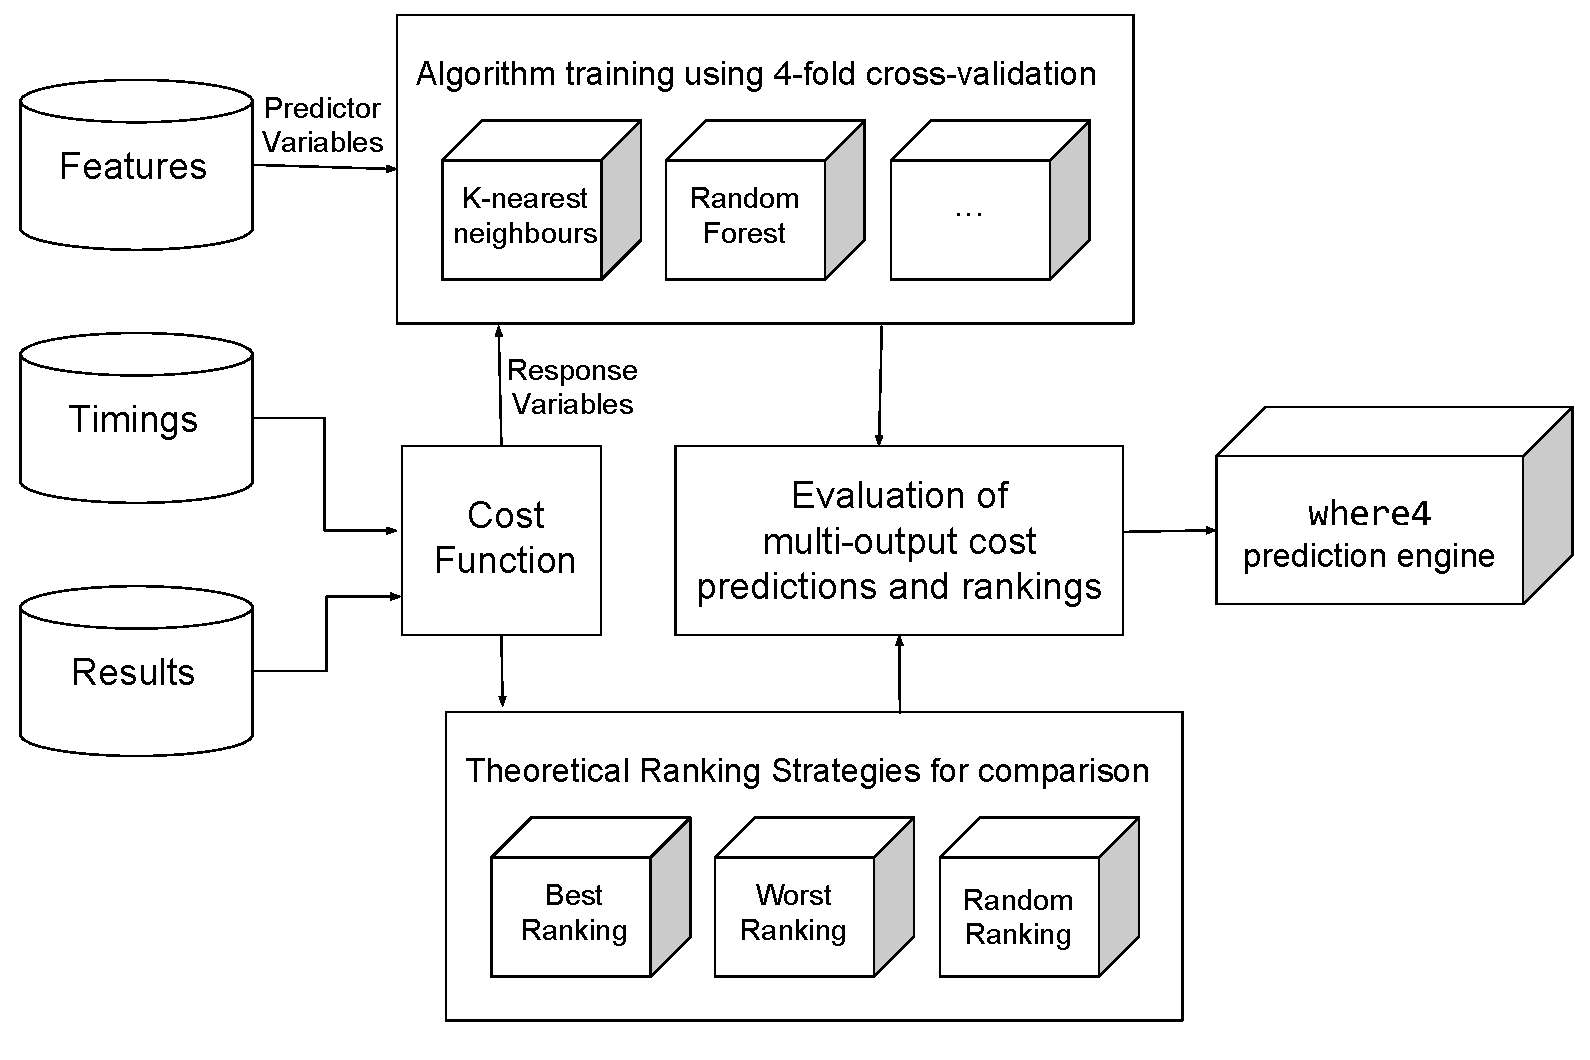
\includegraphics[width=1.0\linewidth]{Figures/Chapter4}
	\caption{Overview of the process used to derive the \textsf{Where4} prediction model}
	\label{fig:Chapter4}
\end{figure}

Fig. \ref{fig:Chapter4} illustrates a high-level view of the process used to compare and evaluate the various ranking strategies in this section. 
The solver timings and results are combined as a single variable using the cost function defined in Sec. \ref{sub:scoring}.
The value returned by this function is the response variable for a number of ML algorithms; with the statically-extracted features acting as the predictor variables.

A four-fold cross validation of this data is used to evaluate the models. 
In this method, the data is split into quarters.
Four models are effectively trained on different datasets by holding a different quarter back for model evaluation each time.
The final evaluation is based on the model's average performance over the four instances.
The general \textit{K-fold} cross validation method allows the use of the entire dataset for model evaluation and training (rather than holding a portion of the data back solely for model evaluation use -- a technique known as ``hold-out'' validation). 
The number of folds used (four) was chosen to reflect the percentage of the total dataset (75\%) used for training. 
The folds were stratified (i.e. ensuring a representative frequency of values was contained in each split) according to the best performing solver for each instance.
This technique was used to overcome the difficulties of stratification for regression tasks where values may appear infrequently.  

\subsection{The ML algorithms we used for model training}

\label{sub:MLalgorithms}
The ML algorithms compared in this section have been briefly introduced in Sec. \ref{sec:lrml}. 
We do not compare Na\"ive Bayes which does not support regression tasks. 
In this section, we go into more detail about how the algorithms operate and the specific variants and parameters chosen for use during this comparison.
We used the Sci-Kit Learn \cite{sklearn} Python implementation for all algorithms.
The consistent API is well-designed, the library is well documented and it integrates well with other Python tools for scientific computing (such as NumPy and the Pandas data structure library).


\subsubsection{ML Algorithm 1: Support Vector Machines}

%As a member of the \textit{analogical} family of learning algorithms, 
Support Vector Machines (SVMs) \cite{svm} are based on a concept of similarity between training instances. 
During training, a number of separating hyperplanes are determined.
The idea behind SVMs is to ensure the distance from this hyperplane to any training instances closest to it is maximal.
This process is known as ``maximising the margin'' and is designed give the model the best chance at classifying unseen instances correctly. 
The set of training instances closest to the margin is called the \textit{support vector} as they can be thought of as ``holding up'' the hyperplane.

A number of kernel functions can be used as a similarity measure during training.
We chose to use the \textit{Radial Bias Function} (RBF) kernel as we can not assume a linear relationship between our features and cost value. 
The RBF kernel requires the use of two hyperparameters to control how flexible the model is (i.e. how closely it fits the training data). 
We used a grid search technique \cite{hsu2003practical} to identify the $C$ (hyperplace smoothness) and $gamma$ (the radius of influence for each individual training instance) parameters.

In the multi-output case, each cost value has to be predicted individually for each solver -- requiring the use of eight SVMs each tuned to different parameters on a per-solver basis.
The benefit of using SVMs is their ability to give good results in large-dimensional spaces; even with large datasets. 

We followed Hsu and Lin's \cite{MulticlassSVM} recommendations regarding the use of SVMs (which excel at \textit{binary} classification) for  multi-output regression tasks. 

\subsubsection{ML Algorithm 2: Decision Trees}

Decision trees recursively construct a binary tree by  splitting the data on the feature and threshold which create the most distinct partitions \cite{DecisionTrees}.
This notion of ``distinctiveness'' is defined using either a measure of entropy or information gain.
Features of new instances are queried according to the thresholds specified by the non-leaf nodes, with leaves consisting of (one or many) predictions. 
The original implementation required that features be categorical (Quinlan's ID3 algorithm). 
Sci-kit Learn uses the CART \cite{cart} algorithm which supports numerical features and outputs for regression tasks.  

Decision trees are a transparent and powerful method for classification and regression.
Since the 1960s, decision trees have been successfully deployed in many domains. 
In the intervening years, techniques have been developed to improve the accuracy and generalisability of decision trees: such techniques include the pruning of \textit{if-then} branches created by sequences of splitting nodes.
Termination conditions can be used to limit the depth of the tree and make each leaf node account for a minimum number of examples in the training data.
We chose this last technique as a method to prevent our decision tree from overfitting training data: a minimum of five training instances had to be described by the \textit{if-then} rule associated with the leaf.
By using this constraint, non-leaf nodes are converted into leaves if, when split, they would have produced leaves of size less than five. 
This relatively small number (five) was chosen as a compromise: leaves of this size allow the decision tree to generalise better than trees with leaves accounting for fewer training instances. 
At the same time, the leaves remain small enough to allow the tree to utilise many of the instance's features for its characterisation (i.e. the tree's depth does not become too small).   

\subsubsection{ML Algorithm 3: Random Forests}

Random forests \cite{RandomForests} were created as a response to decision tree's tendency to overfit training data -- leading to poor generalisation results.
As the name suggests, this technique involves creating many decision trees, with each tree trained on a random subset of the training data and/or restricted to using a subset of the features for use in splitting nodes.
Random forests are an example of an \textit{ensemble} method which uses multiple weak predictors to strengthen the overall prediction.

For classification problems, each tree ``votes'' on an instance's class.
In the regression case, all trees' predictions are averaged to determine the forest's ultimate prediction.   

Similar to our use of decision trees, we limited the depth of each tree by specifying a minimum size of five for each leaf node. 
For this initial algorithm comparison we used 100 trees in the random forest. 
This is the default Sci-Kit Learn implementation.

\subsubsection{ML Algorithms 4 \& 5: Linear and Ridge Regression} 

Linear regression attempts to predict the parameters of a function which fits the input features to the output variable. 
It expects that the output variable be a linear combination of the input variables.
We used the Ordinary Least Squares formulation which attempts to minimise the sum of squared error for the set of training instances to the output variable.    

Ridge regression \cite{ridge} is a related algorithm which attempts to be more robust to violations in the input variables' independence. 

\subsubsection{ML Algorithm 6: k-Nearest Neighbours Clustering}

K-Nearest Neighbours (k-NN) clustering, like SVMs, belong to the analogical family of ML algorithms which rely on a similarity measure to group training instances (we used the standard Euclidean distance).
The idea is to create $k$ clusters of training instances which are ``most similar'' to each other in terms of features -- with each feature acting as a dimension.   
In both the k-NN and SVM algorithms, instances must undergo a normalisation process to scale features.  
This preprocessing step is designed to avoid dominance of one feature over another (due to differences in scale) in distance-based algorithms.
In contrast to SVMs, most clustering algorithms (k-NN included) do not scale well in high-dimensional spaces.

\sloppypar
Typically used for classification tasks, the k-NN algorithm can be adapted for regression by calculating the target/response variable as the average of the $k$ nearest instances in the training data.
By default, Sci-Kit Learn sets $k=5$: each instance is compared to the five most similar instances (in terms of input variables) in the training set.  
We used a modification: training instances ``closer'' to the unseen instances are weighted more than those further away in the cluster when computing the target variable.
This modification makes the algorithm more robust to noisy training data. 

\subsection{Experimental Configuration}
\label{sub:config}

In the previous chapter, we described our dataset as consisting of 1048 \textsf{Why3} POs.
We now split this dataset into two disjoint subsets: the \textit{training} and \textit{testing} sets. 
The rest of this chapter uses only the \textit{training} set while the \textit{testing} set is used in our final evaluation of \textsf{Where4} in Chapter \ref{Evaluation}.
The training set represents 75\% of the entire dataset: 96 files,   212 theories and 785 goals. 
The data was split on a per-file basis to ensure that the no PO in the training set belonged to the same theory or file as a PO in the test set. 

Beside the standard implementation of the prediction algorithm, two variations were evaluated: cost discretisation and instance weighting.
By discretisation we describe the process to transform a continuous-valued variable into one of a finite number of values. 
It usually involves dividing the continuous variable by some small empirically-tested number. 
Discretisation allows algorithms which perform better when given a smaller number of discrete options for prediction to be identified. 
We chose 2.5 to be a discretisation divisor for the response variable (i.e. each solver's cost).
In choosing this value, two factors must be balanced: the discretisation error inherent in the process should be minimised while allowing only a relatively small number of possibilities for prediction.

The other technique we applied during model evaluation was the weighting of training instances\footnote{Apart from K-Nearest Neighbours: the Sci-kit Learn implementation does not support instance weighting.}.
Weighting is standard practice in supervised machine learning: each instances's weight was defined as the standard deviation of solver costs for the PO in question. 
This function was designed to give more importance to instances where there was a large difference in performance among the solvers; thereby de-emphasising trivial POs provable by most or all solvers, and empirically hard instances for which all solvers fail or time out.  


\section{Ranking strategies}
\label{sec:strategies}

The ranking strategies introduced in this section are not directly comparable to single solvers or to theoretical solvers such as \textsf{Choose Single}. 
The purpose of defining these strategies is to provide a basis by which we can compare and evaluate the solver rankings predicted by the ML models.
The \textsf{Best Ranking} and \textsf{Worst Ranking} strategies use the empirical measurements to construct rankings on a per-goal basis, while the \textsf{Random Ranking} strategy uses the same set of rankings for each goal.
We refer to the following strategies as \textit{theoretical} as they assume knowledge of the actual behaviour of the solvers for the goal in question -- knowledge which is impossible to have prior to execution in a real-world verification scenario.     

Algorithm \ref{algo:rank} describes the process to return answers and runtimes from solver rankings. This process is used in our model evaluation (Sec. \ref{sec:pred-results}).
Essentially, the runtime of next best solver (according to a given ranking) is added to the cumulative total until an answer of \textit{Valid} or \textit{Invalid} is returned or the array of solvers has been exhausted. 
When solver answers are compared in the \texttt{if} statement, the ordering of response utility introduced in Sec. \ref{sub:rel-util} (with \textit{Timeout} responses preferred to \textit{Failure}): $\lbrace Valid, Invalid \rbrace > Unknown > Timeout > Failure$.
If both \textit{Valid} and \textit{Invalid} responses were recorded for the same PO, it would indeed signal a soundness bug existed in one of the solvers.
This issue did not arise.  

\begin{algorithm}
	\caption{Returning answers and runtimes from solver rankings}
	\KwIn{Solvers $\lbrace S_1,...,S_n\rbrace$ sorted by cost (predicted, actual, or random)}
	\KwOut{$\langle A,T\rangle$ where $A$ = the best answer from the solvers; $T$ = the cumulative time taken to return $A$}
	\Begin{
		\tcc{initialisation}
		$A \leftarrow Failure$ \\
		$T \leftarrow 0$ \\
		$i \leftarrow 1$ \\
		\While{$A \notin \lbrace Valid, Invalid \rbrace \wedge i \leq n$}
		{
		\tcc{$A_S$ = the answer returned by solver $S_i$}
		$A_S \leftarrow Answer(S_i)$ \\
		\tcc{add solver $S_i$'s time to the cumulative runtime}
		$T \leftarrow T + Time(S_i)$  \\
		\If{$A_S > A$}
		{
			\tcc{$S_i$'s answer is better than the current best answer}
			
			$A \leftarrow A_S$ }
			$i \leftarrow i + 1$}
		\Return{$\langle A,T\rangle$}} 
	\label{algo:rank}
	
\end{algorithm}


\subsection{\textsf{Best Ranking}}
\label{sub:best}

The \textsf{Best Ranking} is the one derived from sorting the solvers in terms of increasing cost. 
Referring to the solver costs listed in Table \ref{table:cost}, the \textsf{Best Ranking} for this goal is
CVC3 > Alt-Ergo-0.95.1 > Alt-Ergo-1.01 > CVC4 > veriT > Z3-4.3.2 > Z3-4.4.1 > Yices. 
As the first-choice solver according to this ranking (CVC3) returns an answer of \textit{Valid}, no other solver will be called after the first returns its answer. 
Thus for the \textit{first\_last} goal, the \textsf{Best Ranking} strategy returns an answer of \textsf{Valid} in 0.356 seconds.   

It is important not to confuse the \textsf{Best Ranking} strategy with the theoretical solver \textsf{Choose Single} introduced in Sec. \ref{sec:portfolio-benefit}. 
\textsf{Choose Single} refers to a \textit{single} solver (and hence is directly comparable to the other eight SMT solvers in Table \ref{table:avgtimes}), while \textsf{Best Ranking} refers to a \textit{ranking} of all eight solvers. \textsf{Choose Single} is equivalent to using the top-ranking solver from \textsf{Best Ranking} and stopping.

\subsection{\textsf{Worst Ranking}}
\label{sub:worst}

Ranks returned by the \textsf{Worst Ranking} strategy are the inverse to those from the \textsf{Best Ranking}. 
For the \textit{first\_last} goal, Yices will be the first solver called by this strategy.
As Yices returns an answer other than \textit{Valid} or \textit{Invalid}, the next solver in the ranking (Z3 version 4.4.1) will be called, and so on.
The user of this strategy would have to wait until the eighth solver, but a \textit{Valid} answer would eventually be returned.
For the example goal, the \textsf{Worst Ranking} strategy returns an answer of \textit{Valid} in 41.349 seconds.

Both the \textsf{Best Ranking} and \textsf{Worst Ranking} strategies provide important upper and lower bounds for any trained model's runtime.
If a goal is provable by any of the eight solvers, all of our theoretical strategies will be able to prove it.
The difference between these strategies is how long the goal takes to be proven.  
\textsf{Worst Ranking} therefore acts as a method to obtain the  \textit{worst case} runtime (which would in fact be equal to that of \textsf{Best Ranking} for POs which cannot be proved by any of the eight solvers).
This point is important to bear in mind when evaluating prediction models (and their implementation in \textsf{Where4}), as a seemingly ineffective ordering may be equivalent to the best ordering of solvers. 


\subsection{\textsf{Random Ranking}}

The \textsf{Random Ranking} strategy differs from the previous two because it does not refer to \textit{one} ranking per goal but to \textit{all possible} rankings for every goal.
The set of all possible rankings is the same for all goals, but the runtime and result obviously vary.
As previously mentioned, there are eight factorial (or 40,320) possible solver rankings.
The runtime for each of the 40,320 rankings is calculated and the mean of these times is returned by \textsf{Random Ranking}.
As mentioned in relation to \textsf{Worst Ranking}, for any goal the result returned by all rankings (of the same eight solvers) is the same.
  
For the \textit{first\_last} goal, the \textsf{Random Ranking} strategy returns an answer of \textit{Valid} in an average time of 20.853 seconds.

\subsection{Quantifying Solver Contributions Using Ranking Strategies}

\sloppypar
In addition to the findings presented in Sec. \ref{sub:rel-util} which measured the goals uniquely provable by each solver, this section quantifies how valuable each individual solver is to a ranking of solvers.
We follow a method described by Xu et al \cite{Xu2012}: each constituent solver $A$'s value is measured by observing the performance of the theoretical best solver which does not include $A$.
Hence, $A$'s \textit{marginal contribution} to \textsf{Best Ranking} can be defined as the difference between \textsf{Best Ranking}'s cumulative cost excluding $A$: $cost(\textsf{Best Ranking}_{-A})$; and its cumulative cost including $A$: $cost(\textsf{Best Ranking})$.
\[
	contrib(A) = cost(\textsf{Best Ranking}) - cost(\textsf{Best Ranking}_{-A})
\]
We define the cost of a ranking to be the cumulative cost for each of its constituent solvers:
for any given PO, we accumulate the cost of each solver called until an answer is returned according to Alg. \ref{algo:rank}.
To ensure $cost(\textsf{Best Ranking}) \leq cost(\textsf{Best Ranking}_{-A})$, the two rankings need to have the same number of solvers. 
Thus, we exclude the lowest ranking solver from \textsf{Best Ranking} for these purposes.
This accounts for POs unprovable by any solver (\textit{Hard} in terms of the data presented in Table \ref{table:unique}) which have a relatively high cost for all solvers. 
Including these costs when comparing rankings would bias the results towards the rankings with fewer solvers: the \textsf{Best Ranking} excluding $A$ will always have a lower cost than the ranking including $A$ for \textit{Hard} POs.   

For each solver in the set of solvers $S$, we normalise its contribution by dividing it by the sum of all solver contributions and multiplying by 100:
\[
	contrib_{norm}(A) = \frac{contrib(A)}{\sum_{i=1}^{|S|} contrib(S_i)} \times 100
\]
\begin{figure}
\centering
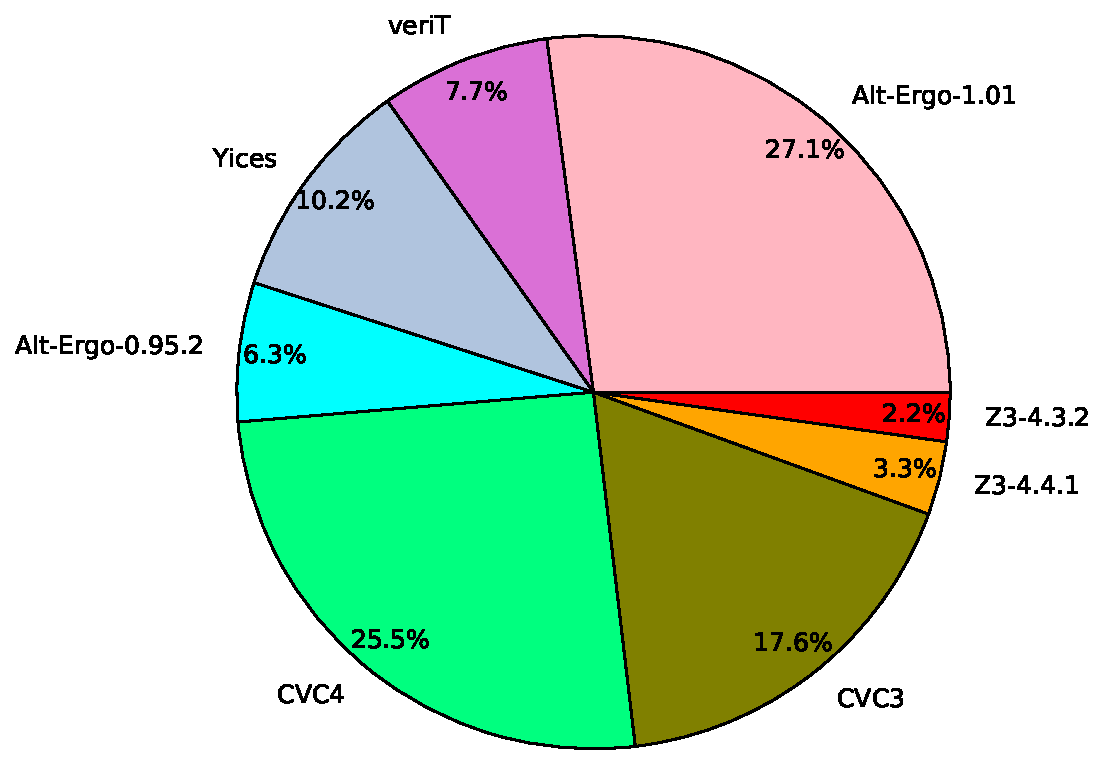
\includegraphics[width=0.8\linewidth]{Figures/pie}
\caption[Relative solver portfolio contributions]{Relative solver portfolio contributions}
\label{fig:pie}
\end{figure}
Figure \ref{fig:pie} shows the normalised contribution statistics for each solver in the portfolio.
Each solver's percentage represents the impact its exclusion has on \textsf{Best Ranking}'s accumulated cost across the entire dataset, relative to the other solvers.
It is unsurprising that Alt-Ergo-1.01 and CVC4 contribute most to the portfolio: these solvers can prove the most uniquely-provable POs (according to Table \ref{table:unique}).  
It is somewhat unexpected that veriT and Yices contribute more than either version of Z3, given that they can prove less goals overall (Table \ref{table:avgtimes}).
This implies that (i) Z3 does not perform significantly better than other solvers for provable goals, (ii) veriT and Yices prove goals in a very short time and (iii) for goals not provable by any of these solvers, veriT and Yices return a better answer in a shorter time.

It is logical that earlier versions of solvers contribute less than more recent versions. 
Alt-Ergo-0.95.2 contributes significantly less than Alt-Ergo-1.01: we deduce that the earlier version takes more time to return a worse answer for \textit{Hard} POs than the update.
Nevertheless, including multiple versions of solvers improves prediction accuracy and ultimately makes \textsf{Where4} a more flexible tool for the user.     


\section{Predictor Selection Results}

\label{sec:pred-results}

In Table \ref{table:predselection} we list the cross-validation results for all six trained prediction models (with discretised and/or weighted variants where applicable).
We compare these  with the three theoretical ranking strategies introduced in Sec. \ref{sec:strategies}.
For each of the five Evaluation Criteria EC1-5, the best-performing algorithm is marked in bold with an asterisk. 

\subsection{EC1: Time}

The first result column, labelled \textbf{Time (secs)}, shows the average time taken for the ranking of solvers returned by the model/strategy to return a \textit{Valid} / \textit{Invalid} response (if such a response was in the set of solver answers -- see Algorithm \ref{algo:rank}).

If there is no \textit{Valid} / \textit{Invalid} response in the set, the time will be the same for any ordering of the solvers (ie. all eight will be called). 
We do not ignore the time taken for the response to be returned.

\subsection{EC2: $R^2$ Score}

The second numeric column of Table \ref{table:predselection} shows
the $R^2$ score (or coefficient of determination), which is an established evaluation criterion. 
It measures how well regression models can predict the variance of dependent / response variables. 
The maximum $R^2$ score is 1 but the minimum can be negative. Note that the theoretical strategies return rankings rather than individual solver costs. 
For this reason, $R^2$ scores are not applicable.

The $R^2$ score is calculated by the following formula
\begin{equation}
\label{r2}
R^2 = 1-\frac{\Sigma(y_i - \hat{y})^2}{\Sigma(y_i - \bar{y})^2}
\end{equation}
which can be interpreted as ``the sum of squared error of the predictions divided by the sum of the squared mean".  
In Formula \ref{r2}, $y_i -\hat{y}$ denotes the distance of the predicted value $\hat{y}$ from the actual value $y$ for data point $i$.
$\bar{y}$ is the mean value from the set of actual values (which in our case is a two-dimensional array of solver scores).
We used the Sci-Kit Learn implementation of this formula, which allows $\bar{y}$ to be set to the weighted average of the outputs for multi-output instances.
We applied uniform weighting to all outputs; meaning the variance of the individual solvers' scores was not considered. 

     



\begin{table}
	\caption[Predictor Selection Results]{ Predictor Selection Results. * indicates the best result among the prediction models }
	
	\begin{adjustbox}{angle=90} 
		\begin{tabularx}{0.9\textheight}{@{}lrrZZZZZ@{}}
			{} & \textbf{Discretised} & \textbf{Weighted} & \textbf{Time (secs)} & $R^2$ & \textbf{nDCG} &  \textbf{MAE} &  \textbf{Reg-error} \\
			\midrule
			\textsf{Best Ranking}  &  &  &     12.59 &    - &  1.00  & 0.00 &        0.00 \\
			\textsf{Random Ranking} & &  &     19.06 &   - &  0.36  & 2.62 &       50.77 \\
			\textsf{Worst Ranking}  & &  &     30.23 &   - &  0.00  & 4.00 &       94.57 \\
			\midrule
			\multirow{4}{*}{Decision Tree}  & \xmark & \xmark     &     16.37 & 0.09 &  0.49 &    2.08 &       45.00 \\
			& \cmark & \xmark     &     15.90 &  -0.18 & 0.43 &  2.27 &       42.65 \\
			& \xmark & \cmark     &     15.81 &  -0.06 & 0.48 &  2.09 &       41.14 \\
			& \cmark & \cmark &     15.75 &  -0.17 & 0.43 &  2.25 &       41.80 \\
			\midrule
			\multirow{2}{*}{k-Nearest Neighbours} & \xmark & \xmark          &     15.40 & 0.17 & \textbf{*0.55} &    \textbf{*1.90} &       40.65 \\
			& \cmark & \xmark          &     15.49 &  -0.19 & 0.44 &  2.26 &       41.47 \\
			\midrule
			\multirow{4}{*}{Linear Regression}  & \xmark & \xmark                        &     15.60 &  -0.11 & 0.41 &  2.45 &       49.70 \\
			& \cmark & \xmark                     &     15.74 &  -0.30 & 0.41 &  2.46 &       49.12 \\
			& \xmark & \cmark                 &     15.78 &  -0.32 & 0.41 &  2.43 &       49.72 \\
			& \cmark & \cmark             &     15.80 &  -0.26 & 0.41 &  2.45 &       50.12 \\
			\midrule
			\multirow{4}{*}{Support Vector Regressor}  & \xmark & \xmark                           &     15.59 &   0.15 & 0.49 &  2.31 &       46.17 \\
			& \cmark & \xmark                        &     15.61 &  -0.23 & 0.43 &  2.31 &       43.17 \\
			& \xmark & \cmark                    &     15.35 &  -0.00 & 0.46 &  2.26 &       41.65 \\
			& \cmark & \cmark                &     15.53 &  -0.19 & 0.44 &  2.26 &       43.17 \\
			\midrule
			\multirow{4}{*}{Random Forest}   & \xmark & \xmark         &     14.99 &  \textbf{*0.28} & 0.48 &   2.09 &       39.63 \\
			& \cmark & \xmark         &     15.04 &  -0.18 & 0.47 &  2.13 &       39.20 \\
			& \xmark & \cmark     &     \textbf{*14.88} &   0.20 & 0.49 &  2.10 &       \textbf{*38.26} \\
			& \cmark & \cmark &     15.03 &  -0.15 &  0.49 & 2.11 &       38.66 \\
			\midrule
			\multirow{4}{*}{Ridge Regression}  & \xmark & \xmark                          &     15.55 &  -0.09 & 0.41 &  2.46 &       49.85 \\
			& \cmark & \xmark                         &     15.65 &  -0.30 & 0.41 &  2.47 &       49.41 \\
			& \xmark & \cmark                     &     15.58 &  -0.08 & 0.40 &  2.49 &       50.12 \\
			& \cmark & \cmark                 &     15.64 &  -0.22 & 0.40 &  2.50 &       50.69 \\
			
		\end{tabularx}
	\end{adjustbox}
	\label{table:predselection}
\end{table}

\subsection{EC3: Normalised Distributed Cumulative Gain}

\label{sub:ndcg}

The third numeric column of Table \ref{table:predselection} shows the 
Normalised Discounted Cumulative Gain (\textbf{nDCG}), which is commonly used to evaluate the accuracy of rankings in the search engine and e-commerce recommender system domains \cite{NDCG}. 
Here, emphasis is placed on correctly predicting items higher in the ranking. For a general ranking of length $p$, it is formulated as:

\begin{equation}
\small
nDCG_p = \frac{DCG_p}{IDCG_p}
\quad\text{ where }\quad
DCG_p = \sum_{i=1}^{p} \frac{2^{rel_i} - 1}{log_2(i+1)}
\label{eq:ndcg}
\end{equation}

where $rel_i$ refers to the relevance of element $i$ with regard to a ground truth ranking, and we take each solver's relevance to be inversely proportional to its rank index.  
In our case, $p = 8$ (the number of SMT solvers).  
The $DCG_p$ is normalised by dividing it by the maximum (or \textit{idealised}) value for ranks of length $p$, denoted $IDCG_p$. 
As our solver rankings are permutations of the ground truth (making $nDCG$ values of zero impossible), the values in Table \ref{table:predselection} are further normalised to the range [0..1] using the lower $nDCG$ bound for ranks of length eight -- found empirically to be 0.4394.

We illustrate our use of this criterion with a small example. 
Take a ground truth ranking of eight items sorted in decreasing relevance as
\[ A > B > C > D > E > F > G > H. \]
We take each item's \textit{relevance} to be inversely-proportional to its rank position:
\[rel_A=8, rel_B=7, rel_C=6, rel_D=5, rel_E=4, rel_F=3, rel_G=2, rel_H=1.\]
The predicted ranking of these items is
\[ B > A > C > F > D > E > G > H .\]
Applying Equation \ref{eq:ndcg} to these values gives us an $nDCG$ value of
\[
\frac{127}{1.0} + \frac{255}{1.58} + \frac{63}{2.0} + \frac{7}{2.32} + \frac{31}{2.58} + \frac{15}{2.81} + \frac{3}{3.0} + \frac{1}{3.17} = 341.053. 
\]
It can be shown that $IDCG_8 = 389.591$ which makes the un-normalised $nDCG$ value for the predicted ranking 0.875. Using the lower bound of 0.4394 to normalise this value to the range $\left[0, 1 \right]$ (accounting for permutations of length 8) gives us a final $nDCG$ score of 0.778. 



\subsection{EC4: Mean Average Error}

Table \ref{table:predselection}'s fourth numeric column shows the 
$MAE$ (Mean Average Error) -- a ranking criterion which can also be used to measure string similarity. It measures the average distance from each predicted rank position to the solver's index in the ground truth.

Using the same predicted and actual rankings as the $nDCG$ example, we calculate the $MAE$ to be:
\[
	MAE = \frac{1 + 1 + 0 + 2 + 1 + 1 + 0 + 0}{8} = 0.75
\]

The Mean Average Error is a good measure of overall ranking accuracy, but it fails to take into account that in many use cases -- including \textsf{Where4} -- it is often the highest-ranking items that are the most important to predict accurately. 

\subsection{EC5: Regression Error}

The rightmost column of Table \ref{table:predselection} (labelled \textbf{Reg. error}) lists the average regression error per instance. 
We illustrate the calculation of the regression error error with a small example. For two testing instances, the predicted and actual costs for three solvers are: 
\[ \left( \begin{array}{ccc}
0.5 & 10.0 & 5.0 \\
0.4 & 5.5 & 10.0  \end{array} \right) = \text{predicted};
\left( \begin{array}{ccc}
0.6 & 9.0 & 8.0 \\
0.7 & 9.5 & 7.0 \end{array} \right) = \text{actual}\]
which gives a per-instance regression error of
\[ \left( \begin{array}{c}
0.1 + 1.0 + 3.0 \\
0.3 + 4.0 + 3.0
\end{array}  \right) = 
\left( \begin{array}{c}
4.1 \\
7.3
\end{array}  \right) \] 
taking the average of the two instances' regression error, 4.1 and 7.3, gives 5.7.
It is this average error between predicted cost and actual cost for eight solvers which is listed in the rightmost column.

The regression error should be treated with a note of caution, however, as the relative ranking of solvers -- which we argue is the most important prediction -- is not explicitly taken into account.
This qualification also applies to the MAE and $R^2$ score criteria. 
Note that when the predictions and actual costs are sorted in increasing order the best-performing solver is predicted correctly for both instances in the previous example.
The entire ranking of solvers is predicted correctly in the first instance.

\subsection{Properties of multi-output problems}
\label{sub:multi}

An interesting feature of all the best-performing models in Table \ref{table:predselection} -- Random Forests, K-Nearest Neighbours, Decision Trees -- is their ability to predict \textit{multi-output} variables. 
In contrast to Support Vector Machines, for example, which must predict the cost for each solver individually, an algorithm which supports multi-output problems can predict each solver's cost simultaneously. 
Not only is this method more efficient (by reducing the number of estimators required), but it has the ability to account for the correlation of the response variables. 
This is a useful property in the software verification domain where certain goals are not provable and others are trivial for SMT solvers. 
Multiple versions of the same solver can also be expected to have highly correlated scores.

A more general survey of multi-output regression and how various ML algorithms can either be adapted or extended for this use case is provided by Borchani et al. \cite{multisurvey}.

\subsection{The chosen model}
\label{sec:chosen}


\begin{table}
	\caption[Relative importance of features for \where]{Relative importance of each feature in the \textsf{Where4}Random Forest model}
	
	
	\begin{tabularx}{\textwidth}{@{}lr|c|lr@{}}
		\toprule
		\textsc{Feature} & \textsc{Importance (\%)} & & 
		\textsc{Feature} & \textsc{Importance (\%)}  \\
		\midrule
		\texttt{func} & 19.63 & & \texttt{divisor} & 2.66 \\
		\texttt{avg-op-arity} &  11.05 & & \texttt{n-ops} & 2.48 \\
		\texttt{int} & 8.96 & & \texttt{not} & 1.15 \\
		\texttt{forall} & 7.19 & & \texttt{if} & 1.07 \\
		\texttt{and} & 6.02 & & \texttt{case} & 0.99 \\
		\texttt{depth} & 5.70 & & \texttt{wild} & 0.84 \\
		\texttt{var} & 4.84 & & \texttt{false} & 0.37 \\
		\texttt{impl} & 4.72 & & \texttt{or} & 0.36 \\
		\texttt{size} & 4.31 & & \texttt{iff} & 0.33 \\
		\texttt{let} & 4.03 & & \texttt{eps} & 0.13 \\
		\texttt{n-quants} & 3.70 & & \texttt{true} & 0.12 \\
		\texttt{n-preds} & 3.27 & & \texttt{exists} & 0.07 \\
		\texttt{zero-ar} & 3.03 & & \texttt{float} & 0.00 \\
		\texttt{n-branches} & 2.97 & & \texttt{as} & 0.00 \\
		\bottomrule	
	\end{tabularx}
	\label{table:importances}
\end{table}


After inspecting the results for all trained models (summarised in Table \ref{table:predselection}), we can see that Random Forests \cite{RandomForests} perform well, relative to other methods. 
They score highest for three of the five criteria (shown in bold with an asterisk) and have generally good scores in the others.
Based on these results, we selected Random Forests as the choice of algorithm to use in \where.
We chose to implement a Random Forest model which does not use discretisation or instance weighting. 
Inspecting the results from the entire range of algorithms shows that, in general, the best-performing models do not use these techniques.

The k-Nearest Neighbours model, while coming top for two important criteria, scored poorly in the \textbf{Time} category.
This result leads us to conclude that k-Nearest Neighbours can often predict good rankings but the instances on which it performs badly are very expensive in terms of time.
Overall, the Random Forest model is the most consistent and reliable predictor.

Before discussing the implementation of \textsf{Where4}in the next chapter, we shall investigate the properties of the Random Forest model after it was fit on the entire training dataset.

Table \ref{table:importances} shows the relative importance of each predictor variable for decision-making in the Random Forest model. 
Every time a split of a node is made on a feature the impurity criterion for the two descendent nodes is less than the parent node. 
This criterion is called the \textit{Gini impurity} \cite{RandomForests}. 
The percentages correspond to the proportion of the \textit{Gini} decrease accounted for splitting by each feature.
This data is part of Sci-Kit Learn's implementation of Decision Trees and Random Forests. 

It can be seen that the number of functions in each PO is the by far the most important factor in determining each solver's cost, with the average branching factor of functions and other operators also being important.
It is somewhat surprising that the number of integer constants is one of the more important factors while the number of floating point constants is relatively unimportant.
This may be due to the fact that there are more integer-based POs in our dataset than those which use floating point numbers.
This reasoning may also account for the fact the universal quantifiers (\texttt{forall}) rank higher than existential (\texttt{exists}) quantifiers.



\section{Summary}

This chapter began by motivating the use of portfolio-solving in the \textsf{Why3} system by showing that more files, theories and goals can be proven by using the best-performing solver on a per-goal basis.
We then gave a tour of the prediction approaches considered for use in \where.
We decided to use a regression method to predict each solver's \textit{cost} -- a value designed to account for solver response as well as the time taken to return the response. 

A number of ranking strategies and evaluation criteria were described in Sec. \ref{sec:strategies} and Sec. \ref{sec:pred-results} respectively.
%We will encounter these concepts again during the evaluation of \textsf{Where4}on test data in Chapter \ref{Evaluation}.
In this chapter, we used them to compare various trained models and found Random Forests to be the best choice for implementation in \where.

Some properties of the trained Random Forest model were then discussed.
The choice of prediction model has an obvious importance on \where's  implementation and success as a predictor. 
We give more details of this implementation in the next chapter.  



 
\chapter{OCaml Implementation}
\thispagestyle{nohead}
\label{Implementation}

This brief chapter will give some details of the choices we made when implementing the \where~tool.
We decided to make \where~available as a stand-alone tool on the command-line as well as through the \why~system by imitating an orthodox SMT solver.   

The implementation of \where~makes use of various techniques and heuristics encountered when researching related premise selection and portfolio solving tools such as those described in sections \ref{sub:lrsvml} and \ref{sub:lrsvmmml} of the Literature Review.   
For example, \where's interaction with \why~is inspired by Sledgehammer's MaSh \cite{Sledgehammer} tool. MaSh uses machine learning to suggest premises based on a large corpus of learned theorems, allowing POs to be proved automatically by ATP and SMT tools. 
We aspired to Sledgehammer's ``zero click, zero maintenance, zero overhead'' philosophy in this regard: \where~should not interfere with a \why~user's normal work-flow nor should it penalise those who do not use it.

One heuristic we implemented was to call the highest ranking solver installed on the user's system from the following static ranking:
$ \text{Alt-Ergo-1.01} > \text{CVC4} > \text{CVC3} > \text{Z3-4.4.1} > \text{Alt-Ergo-0.95.1} > \text{Z3-4.3.2} > \text{Yices} > \text{veriT} $.
We derived this ranking from the total number of POs each solver could prove (as listed in Table \ref{table:avgtimes}).
Using an initial high-performing solver (with a short time limit value) discharges easy POs without incurring the cost of feature extraction and solver rank prediction.
This heuristic is implemented successfully in the SATzilla  \cite{SATzilla2012} portfolio solver for SAT instances where it is termed ``pre-solving''.
SATzilla has inspired the use of pre-solving in portfolio solvers for constraint / optimisation problems such as sunny-cp \cite{sunny-cp}.
This heuristic improves \where's performance and reduces its reliance on the underlying random forest prediction model. 
The process described in Algorithm \ref{algo:rank} for obtaining results from solver rankings needs to be modified to describe \where's operation:
the following algorithm (Alg. \ref{algo:where4}) only performs feature extraction if the initial solver does not solve the input program within 1 second. 

\begin{algorithm}
	\caption{Returning an answer and runtime from a \why~input program}
	\KwIn{$P$, a \why~program; \\ 
		$R$, a static ranking of solvers for pre-proving; \\
		$\phi$, a timeout value}
	\KwOut{$\langle A,T\rangle$ where\\$A$ = the best answer from the solvers;\\
	$T$ = the cumulative time taken to return $A$}
	\Begin{
		\tcc{Highest ranking solver installed locally}
		$S \leftarrow BestInstalled(R) $ \\			
		\tcc{Call solver $S$ on \why~program $P$ with a timeout of 1 second}	
		$\langle A,T \rangle \leftarrow Call(P, S, 1)$ \\
		\If{$A \in \lbrace Valid, Invalid \rbrace $}
			{\Return{$\langle A,T \rangle$}}
		\tcc{extract feature vector $F$ from program $P$} 
		$F \leftarrow ExtractFeatures(P) $ \\
		\tcc{$R$ is now based on program features}
		$R \leftarrow PredictRanking(F) $ \\		
		\While{$A \notin \lbrace Valid, Invalid \rbrace \wedge R \neq \emptyset$}
		{
			$S \leftarrow BestInstalled(R) $ \\	
			\tcc{Call solver $S$ on \why~program $P$ with a timeout of $\phi$ seconds}	
			$\langle A_S,T_S \rangle \leftarrow Call(P, S, \phi)$ \\
			\tcc{add time $T_S$ to the cumulative runtime}
			$T \leftarrow T + T_S$  \\
			\If{$A_S > A$}
			{
				\tcc{answer $A_S$ is better than the current best answer}		
				$A \leftarrow A_S$ }
			\tcc{remove $S$ from the set of solvers $R$}
			$R \leftarrow R \setminus \lbrace S \rbrace$}
		\Return{$\langle A,T\rangle$}} 
	\label{algo:where4}
	
\end{algorithm}

\section{Encoding the random forest}

We train the Random Forest model described in Sec. \ref{sec:chosen} on the entire training set.
The Sci-kit Learn library allows the constituent decision trees to be extracted and inspected.
We print the forest as a JSON array of trees using the data model shown in Fig. \ref{fig:json}. 
%Each \texttt{Forest} consists of an array of \texttt{Trees}, which in turn consist of an array of \texttt{Nodes}. Each node has a unique identifier which is used for navigating the tree. A \texttt{

\begin{figure}
\centering
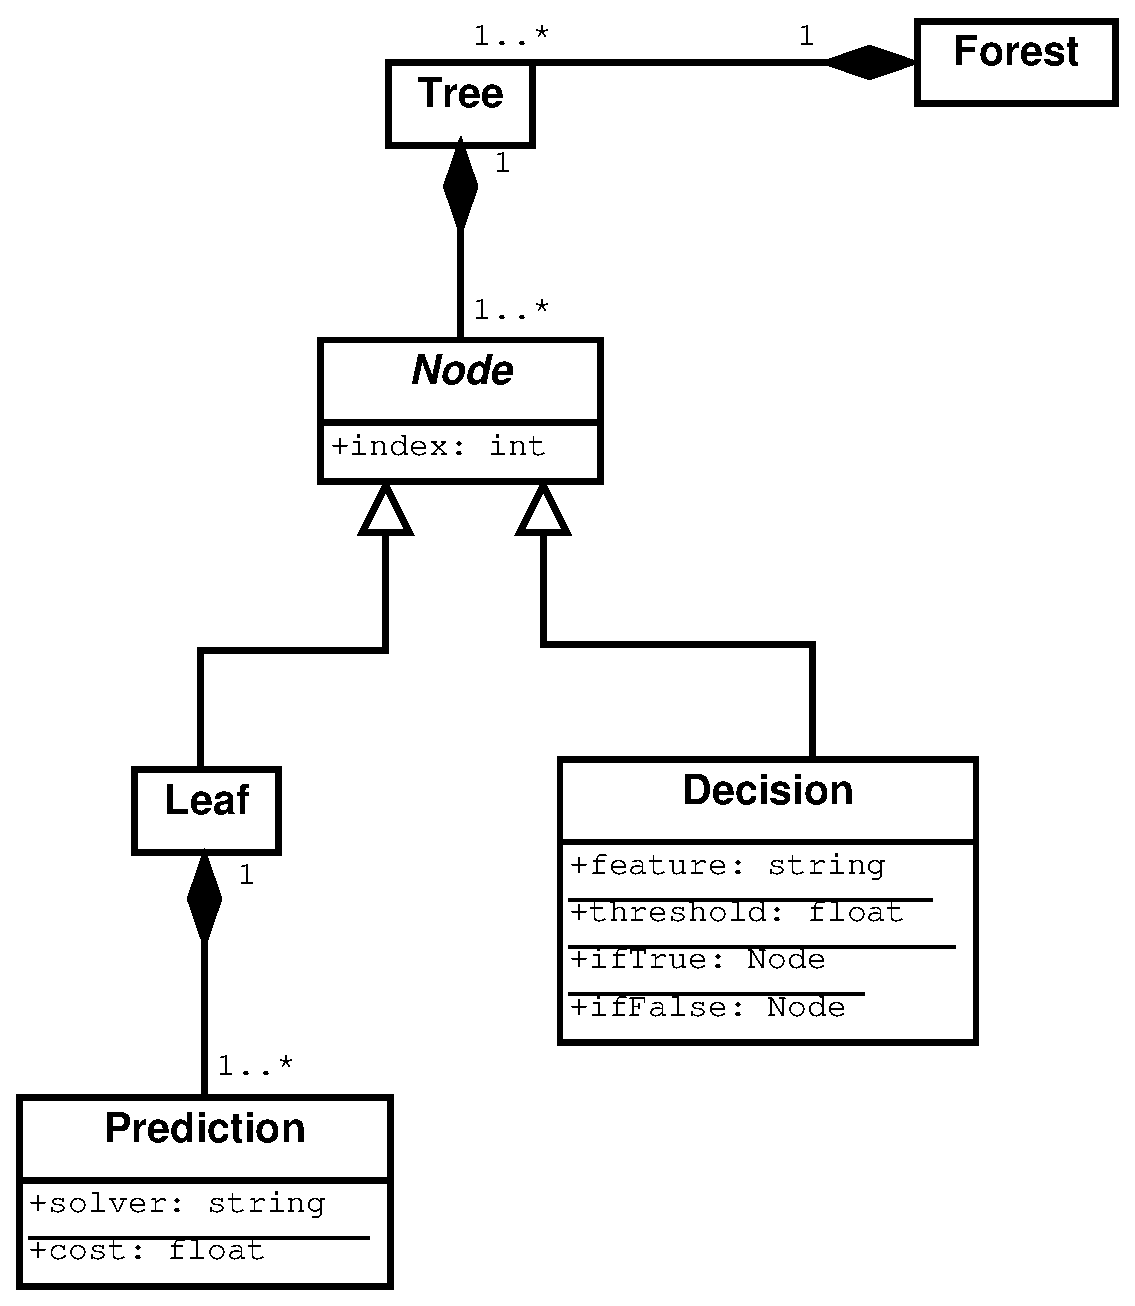
\includegraphics[width=0.8\linewidth]{Figures/data}
\caption[Data design for JSON encoding]{Data design for JSON encoding}
\label{fig:json}
\end{figure}
%
%
%\begin{tabularx}{0.8\textwidth}{@{}ZcY@{}}
%	$forest$ &:=&  $tree^+$ \\
%	$tree$ &:=& $node^+$ \\
%	$node$ &:=& $leaf\,|\, decision$ \\
%	$leaf$ &:=& $(index, prediction^+)$ \\
%	$decision$ &:=& $(index, feature, threshold, true, false)$ \\
%	$prediction$ &:=& $(solver, cost)$ \\
%	$index$ &:=& \texttt{integer} \\
%	$feature$ &:=& \texttt{string} \\
%	$threshold$ &:=& \texttt{float} \\
%	$true$ &:=& \texttt{integer} \\
%	$false$ &:=& \texttt{integer} \\
%	$solver$ &:=& \texttt{string} \\
%	$cost$ &:=& \texttt{float} \\	
%\end{tabularx}

This JSON schema is designed to be human-readable so that users can define their own simple trees in order to experiment with the effect a particular \texttt{feature} may have.
The \texttt{index} attribute is a unique identifier used when traversing the tree: if the value for \texttt{feature} is less than or equal to \texttt{threshold}, the current focus moves to the \texttt{Node} with the value of \texttt{ifTrue}, or to \texttt{ifFalse} if it is greater.
This process continues until a \texttt{Leaf} node is encountered and each solver's cost \texttt{Prediction} is returned.

Fig. \ref{fig:Chapter5} shows \where's design in terms of OCaml modules.
The functions exposed by the interface files (\texttt{*.mli}) are listed in Appendix \ref{App:interfaces}. 
Upon installation of \where, \texttt{forest.json} is read in by \texttt{print\_tree.ml} and an equivalent OCaml array is generated and written to the file \texttt{tree.ml}.
When \texttt{make\_predictions.ml} is provided with a vector of program features by \texttt{where4.ml}, the forest is traversed  in the manner outlined above.
Making the forest available as an OCaml data structure (through the \texttt{tree.mli} interface file) is more efficient than reading in the JSON file at each execution of \where.
Of course, if \texttt{forest.json} changes, \where~needs to be re-installed for these changes to have effect (more information about installing \where~is given in Appendix \ref{App:install}).  


\begin{figure}
	\centering
	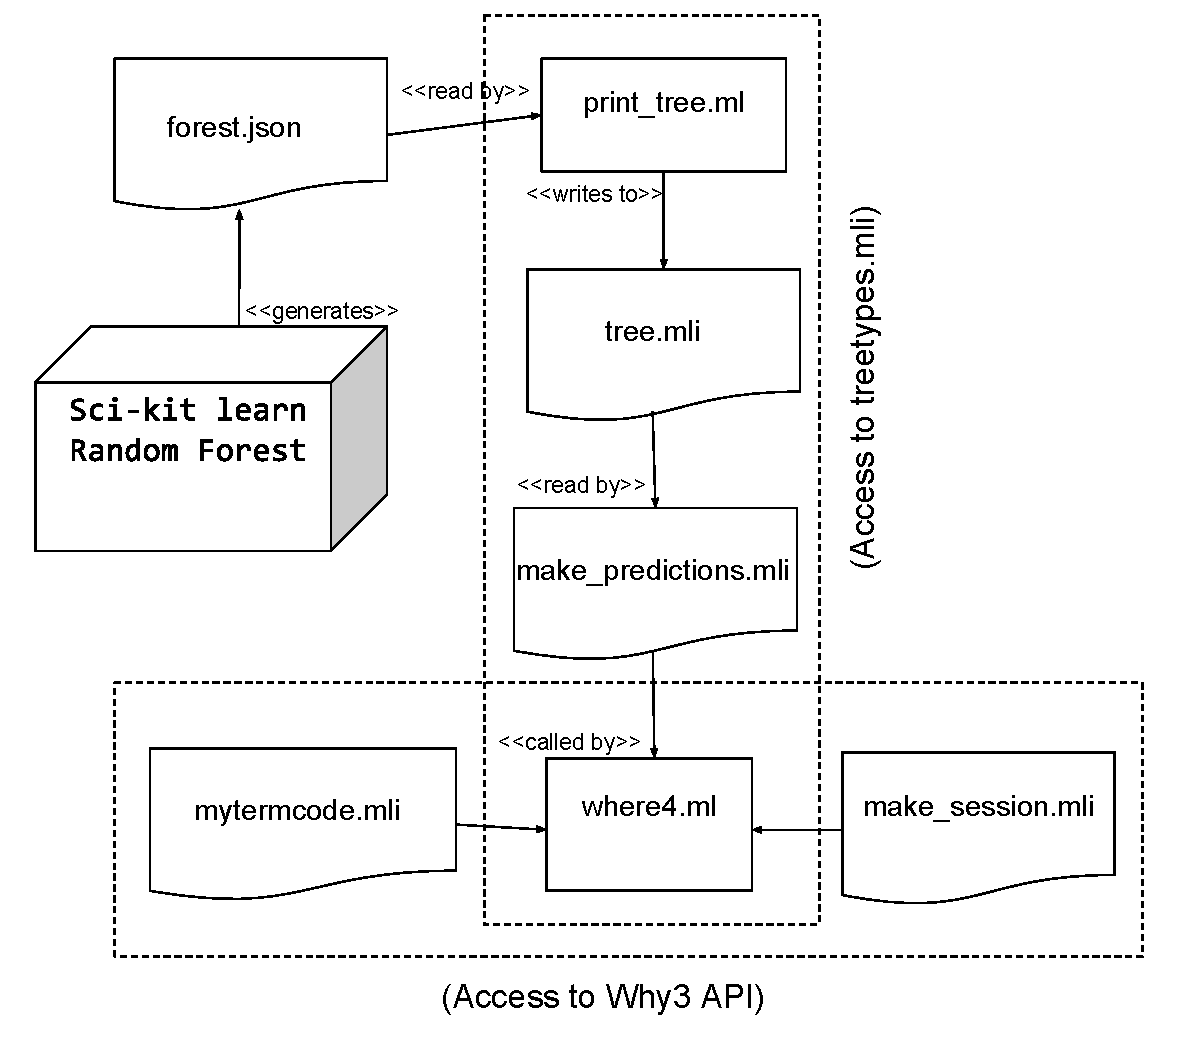
\includegraphics[width=1.0\linewidth]{Figures/Chapter5_stereo}
	\caption[\where~modules]{The organisation of components in \where's design}
	\label{fig:Chapter5}
\end{figure}

\section{Extracting features}

The previous section described \where's use of a tree data structure to predict solver performance given a vector of program features.
A tree is also used to derive these feature vectors from \why~programs: the \why~API is used to traverse the abstract syntax tree (AST) for each PO.
As previously discussed in Sec. \ref{sec:independant}, we use a process similar to that used internally by \why~to extract ``goal shapes'' \cite{why:preserving}.
The \why~Ocaml module to perform this task is named \texttt{termcode.ml} and \where's \texttt{mytermcode.ml} is based upon the same process.

A hash table is maintained while recursively traversing the AST: at each node visited the count of the corresponding feature is incremented in the hash table. 
Any other information (such as function arity, for example) is also recorded before the rest of the tree is traversed. 

\section{Integration with \why}
\label{sec:why3-integration}

The \texttt{mytermcode.mli}, \texttt{where4.ml} and \texttt{make\_session.mli} files are shown in Fig. \ref{fig:Chapter5} as having access to the \why~API. 
We have already described how \texttt{mytermcode.ml} uses the AST to extract the feature vector.
Other important information required by \why~is gathered by the \texttt{make\_session.ml} module.
For example, this module reads the \why~configuration file to determine which supported SMT solvers are installed locally.
\texttt{make\_session.ml} loads drivers for these solvers and creates a proof session in the current directory. This module reads and type-checks the input file; returning its abstract representation.
These actions are performed using a method described by the \why~manual\footnote{Specifically \url{http://why3.lri.fr/doc-0.87.2/manual005.html\#sec28} (last accessed 16/10/16)} \cite{why:manual}.

\texttt{where4.ml} parses command line options (see Appendix \ref{App:command}) and is summarised by Algorithm \ref{algo:where4}.
The imitation of an orthodox SMT solver requires a number of modifications and extra files as follows:
\begin{itemize}
	\item An entry to the \texttt{provers-detection-data.conf} configuration file must be made for \why~to recognise \where~ as a supported SMT solver.
	\where's entry lists the command needed to invoke the binary, specifies which version of the tool is supported, and where to find the corresponding driver file
	\item The driver file must contain regular expressions to parse \where's output, making it comprehensible to \why~(defining the characteristics of a \textit{Valid} output, for example). 
	The driver must also list the printer used by \why~for intermediate files, as well as any transformations which need to be performed to conform to the solver's input language. \where~uses the standard \why~printer and its list of transformations.
	\item The \why~API requires that supplied paths to input files are relative to the current directory. When called via the driver, however, a temporary file is written by the printer and an absolute path is specified. \where~needs to convert this to a relative path in order to read the input file.     
\end{itemize}

These modifications allow \where~to be recognised as an orthodox solver which can be used by \why~through the IDE, on the command-line, or even through the OCaml API. 

\section{Summary}

This chapter has presented an overview of the method we used to implement the \where~tool using the \why~OCaml API.
In total, the six statically-written OCaml modules (i.e. not including \texttt{tree.ml}) contain 712 lines of code.
We used OCaml version 4.02.3 for their compilation locally.
The only library we used (in addition to version 0.87.1 of the \why~API) is Yojson\footnote{version 1.2.1 \url{http://mjambon.com/yojson.html}}  to help with parsing the \texttt{forest.json} file. 
The data disk included with this thesis contains all the source code for \where. 
The files \texttt{install.sh} and \texttt{readme.md} contain useful information about the compilation of these modules and how to satisfy their few dependencies.
The same source files are available online at \url{https://github.com/ahealy19/where4}.

 
\chapter{Evaluating \where~on Test Data}% Main chapter title
\thispagestyle{nohead}
\label{Evaluation} 
%----------------------------------------------------------------------------------------

This chapter will evaluate \where's portfolio algorithm on the held-back test data.
The randomly-selected test set represents 25\% of the entire number of POs and consists of 32 WhyML files, 77 theories and 263 goals  (see Sec. \ref{sub:config}).
In addition to evaluating \where~'s \textit{predictions}, the OCaml implementation (detailed in the previous chapter) will be discussed in terms of its efficiency.   
We also present the results of our prediction algorithm on the training data when no pre-solver is used (i.e. Algorithm \ref{algo:rank} is used).
We do this to evaluate the prediction model in isolation and compare \where's performance with and without the pre-solving heuristic.
We perform our evaluation guided by three Evaluation Questions:
\begin{itemize}
	\item[EQ1:] \textbf{How does \where~perform in comparison to the eight SMT solvers?}\\
	The importance of this question is obvious: the success of \where~depends on its improvement over the status quo. In the case of discharging \why~POs, the status quo is represented as the use of a single solver.
	\item[EQ2:] \textbf{How does \where~perform in comparison to the three theoretical strategies?}\\
	The theoretical strategies introduced in Sec. \ref{sec:strategies} provide a fairer basis for comparison than a single solver by taking multiple solver calls per PO into consideration.
	As a reminder for the reader, the \textsf{Best Ranking} always chooses solvers in the order of ascending cost, \textsf{Random Ranking} is the average result of running \textit{every} possible permutation of the eight solvers, and \textsf{Worst Ranking} is the inverse of \textsf{Best Ranking}: it is the ranking of solvers in order of \textit{descending} cost. 
	\item[EQ3:] \textbf{What is the time overhead of using \where~to prove \why~goals?}\\
	The feature extraction and solver scheduling processes incur a time cost. This evaluation criterion measures whether this cost represents a significant proportion of \where~'s overall solving time.    	
\end{itemize}
%The chapter is organised around answering questions raised by each of the three criteria in turn.
This chapter answers each Evaluation Question in turn.
Threats to the validity of our study are discussed in Sec. \ref{sec:threats}. 

\section{EQ1: How does \where~perform in comparison to the eight SMT solvers?}

\label{sec:eq1}

\begin{table}
	\caption[Results for eight solvers, \where~and three strategies on test set]{Number of files, theories and goals proved by each strategy and individual solver. The percentage this represents of the total 32 files, 77 theories, 263 goals, and the average time in seconds, are also shown.}
	\begin{tabularx}{1.1\textwidth}{@{}l|ZZZ|ZZZ|ZZZ@{}}
		\toprule
		{} & \multicolumn{3}{c|}{\textbf{File}} & \multicolumn{3}{c|}{\textbf{Theory}} & \multicolumn{3}{c}{\textbf{Goal}} \\
		{} & \# proved & \% proved & Avg time & \# proved & \% proved & Avg time & \# proved & \% proved & Avg time \\
		\midrule
		\where~(PS) & 11 & 34.4\% & 1.39 &  44 & 57.1\% & 0.99 & 203 & 77.2\% & 1.98 \\
		\where~(no PS) & \downbar & \downbar & 1.99 & \downbar & \downbar & 1.31 & \downbar & \downbar & 2.32 \\
		\textsf{Best Rank.} & \downbar  & \downbar & 0.25 & \downbar & \downbar & 0.28 & \downbar & \downbar & 0.37 \\
		\textsf{Random Rank.} & \downbar & \downbar & 4.19 & \downbar & \downbar & 4.02 & \downbar & \downbar & 5.70 \\
		\textsf{Worst Rank.} & \upbar & \upbar & 14.71 & \upbar & \upbar & 13.58 & \upbar & \upbar & 18.35 \\
		%\textbf{\textsf{Where4} (tree)} & '' & '' & 4.08 & '' & '' & 2.52 & '' & '' & 3.50 \\
		\midrule
		\textbf{Alt-Ergo-0.95.2} & 8 & 25.0\% & 0.78 & 37 & 48.1\%& 0.26 & 164 & 62.4\% & 0.34 \\ 
		\textbf{Alt-Ergo-1.01} & 10 & 31.3\% & 1.07 & 39 & 50.6\% & 0.26 & 177 & 67.3\% & 0.33 \\ 
		\textbf{CVC3} & 5 & 15.6\% & 0.39 & 36 & 46.8\% & 0.21 & 167 & 63.5\% & 0.38 \\ 
		\textbf{CVC4} & 4  & 12.5\% & 0.56 & 32 & 41.6\% & 0.21 & 147 & 55.9\% & 0.35 \\ 
		\textbf{veriT} & 2 & 6.3\% & 0.12 & 24 & 31.2\% & 0.12 & 100 & 38.0\% & 0.27 \\ 
		\textbf{Yices} & 4 & 12.5\% & 0.32 & 32 & 41.6\% & 0.15 & 113 & 43.0\% & 0.18 \\ 
		\textbf{Z3-4.3.2} & 6 & 18.8\% & 0.46 & 31 & 40.3\% & 0.20 & 145 & 55.1\% & 0.37 \\ 
		\textbf{Z3-4.4.1} & 6 & 18.8\% & 0.56 & 31 & 40.3\% & 0.23 & 145 & 55.1\% & 0.38 \\ 
		\bottomrule
	\end{tabularx}
	\label{table:avgtimes2}
\end{table}

\begin{figure}
	\centering
	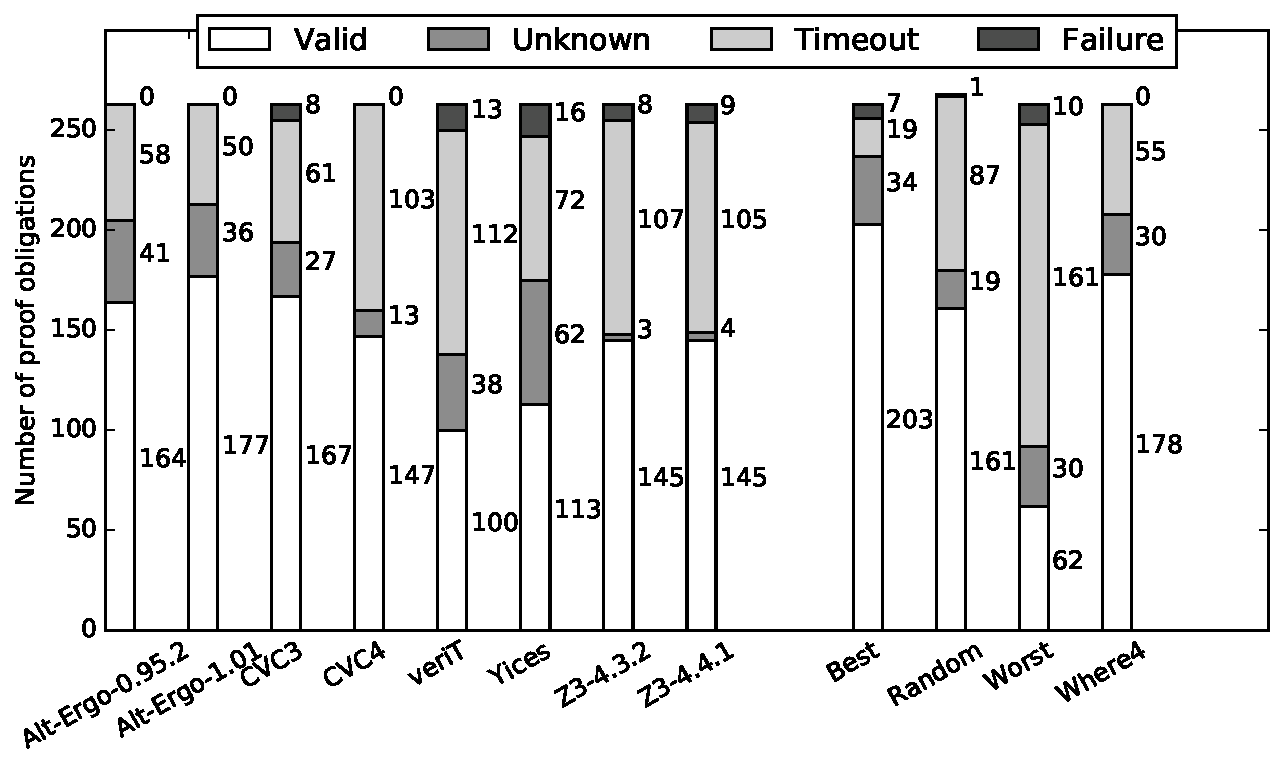
\includegraphics[width=\linewidth]{barcharts2}
	\caption[The relative amount of Valid/Unknown/Timeout/Failure answers from the eight SMT solvers and the top-ranking solver from the three theoretical strategies and \where~(w/(o) presolving).]{The relative amount of Valid/Unknown/Timeout/Failure answers from the eight SMT solvers, \where~(PS where pre-solver = Alt-Ergo-1.01), \where~with no Pre-Solver, and three theoretical strategies on the 263 test POs (with a timeout limit of ten seconds).}
	\label{fig:barchart2}
\end{figure}


When each solver in \textsf{Where4}'s ranking sequence is run on each goal, the maximum amount of files, theories and goals are provable. 
As previously mentioned in Sec. \ref{sub:worst} and as Table \ref{table:avgtimes2} shows, the difference between \where~and the set of reference theoretical strategies (\textsf{Best Ranking}, \textsf{Random Ranking}, and \textsf{Worst Ranking}) is the amount of time taken to return the \textit{Valid/Invalid} result. 
Compared to the eight SMT solvers, the biggest increase is on individual goals: \textsf{Where4} can prove 203 goals, which is 26 (9.9\%) more goals than the next best single SMT solver, Alt-Ergo-1.01.

As is shown by Table \ref{table:avgtimes2}, the average time taken for \textsf{Best Ranking} to return an answer of \textit{Valid} is not necessarily less than that of an individual solver. 
As \textsf{Best Ranking} can return \textit{Valid} for all provable POs -- more than any individual solver --
it is the number of \textit{Valid} answers, rather than any inefficiency, that is responsible for this slightly slower average time.  

The average time \where~takes to prove these goals 
(using Algorithm \ref{algo:where4} -- denoted \where~(PS) in Table \ref{table:avgtimes2}) 
is significantly better than the \textsf{Random Ranking} strategy.
Without a pre-solver, \where~suffers slightly (as denoted by the results for \where~(no PS)). 
Both algorithms, however, lag behind the time recorded by the \textsf{Best Ranking} strategy. 

In comparison to the eight SMT solvers, the average time taken by \where~to prove each of the 203 goals is high. 
This tells us that \where~can perform badly with goals which are not provable by many SMT solvers: expensive \textit{Timeout} results are chosen before the \textit{Valid} result is eventually returned. 
In the worst case, \where~may try all eight solvers in sequence, timing out for each solver, whereas each individual solver does this just once. 
Thus, while having access to more solvers can allow more goals to be proved (if there are goals uniquely-provable by the solvers such as those identified in Table \ref{table:unique}), there is also a time penalty associated with portfolio-based solvers in these circumstances.
This issue has previously been identified by Amadini et al. in their studies on portfolio solvers for constraint programming \cite{Amadini2013} and constraint optimisation \cite{Amadini2016} where portfolio performance was found to degrade as the number of constituent solvers increased.

The multiple timeout issue raises the question of whether it is fair to compare \where~to individual solvers. 
Any ranking strategy will be able to prove the maximum number of files, theories and goals, but unless the best solver is consistently placed high in the ranking, it could take a significantly longer time to do so than even the worst-performing individual solver.   

We remind the reader of the \textsf{Choose Single} solver introduced in Sec. \ref{sec:portfolio-benefit}.
\textsf{Choose Single} is the \textit{best single solver} as chosen on a per-goal basis.
It provided a motivation for the use of portfolio-solving on the \why~platform by proving the maximum number of goals in the shortest amount of time.
We mentioned that \textsf{Choose Single} is equivalent to choosing  the top-ranking solver from \textsf{Best Ranking} and stopping.
We return to this concept in Fig. \ref{fig:barchart2} which is similar to Fig. \ref{fig:barcharts} in that it shows the relative amount of \textit{Valid/Unknown/Timeout/Failure} answers from the eight SMT solvers. 
Also shown (on the right) are results obtainable by using the top solver (only) with the three ranking strategies (where \textsf{Best Ranking} $\equiv$ \textsf{Choose Single}) and the \where~predicted ranking (after pre-solving with Alt-Ergo version 1.01 -- \where~(PS) -- and without: \where~(no PS)).


\begin{algorithm}
	\caption{Returning answers and runtimes from \where~solver rankings using a cost threshold: A minor modification to Alg. \ref{algo:where4} with an additional stopping condition in the \textbf{while} loop}
	\KwIn{$P$, a \why~program;\\ 
		$R$, a static ranking of solvers for pre-proving; \\
		$\phi$, a timeout value; \\ 
		$\mu$, the cost threshold}
	\KwOut{$\langle A,T\rangle$ where \\
		$A$ = the best answer from the solvers; \\
		$T$ = the cumulative time taken to return $A$}
	\Begin{
		\tcc{pre-solving}
		$S \leftarrow BestInstalled(R) $ \\				
		$\langle A,T \rangle \leftarrow Call(P, S, 1)$ \\
		\If{$A \in \lbrace Valid, Invalid \rbrace $}
		{\Return{$\langle A,T \rangle$}}
		$F \leftarrow ExtractFeatures(P) $ \\
		$R \leftarrow PredictRanking(F) $ \\
		\tcc{the predicted cost of $S$ is an additional stopping condition}
		\While{$A \notin \lbrace Valid, Invalid \rbrace \wedge R \neq \emptyset \wedge Cost(S) \leq \mu$}
		{$S \leftarrow BestInstalled(R) $ \\	
			$\langle A_S,T_S \rangle \leftarrow Call(P, S, \phi)$ \\
			$T \leftarrow T + T_S$  \\
			\If{$A_S > A$}
			{	
				$A \leftarrow A_S$ }
			\tcc{remove $S$ from the set of solvers $R$}
			$R \leftarrow R \setminus \lbrace S \rbrace$}
		\Return{$\langle A,T\rangle$}}
	\label{algo:threshold}
	
\end{algorithm}

The 62 \textit{Valid} answers returned by the top solver from the \textsf{Worst Ranking} (i.e. the worst solver) represent the trivial POs solvable by all eight solvers. 
Likewise, the 60 goals for which \textsf{Best Ranking} did not return a \textit{Valid} or \textit{Invalid} answer could not be proved by any solver.

The results show that limiting the portfolio solver to just using the best predicted individual solver eliminates the multiple time-out overhead yet reduces the number of goals provable by \where.
This number of goals -- 184 -- is still more than the best-performing individual SMT solver, Alt-Ergo version 1.01.  

In an effort to compare \where~to individual SMT solvers, Table \ref{table:avgtimes2} and Fig. \ref{fig:barchart2} show results at two extremes of a spectrum: using all solvers available, and only using one.
In the next subsection we describe a method to calibrate the use of \where~by using the predicted cost of each solver. 


\subsection{Use of a cost threshold}
\label{sub:threshold}

To balance the time-taken-versus-goals-proved trade-off associated with the two approaches above, we introduce the notion of a \textit{cost threshold} as another method of comparing \where~to individual SMT solvers.
\where's use of a cost threshold constitutes a minor adjustment to Alg. \ref{algo:where4} and is detailed in Alg. \ref{algo:threshold}. 
After pre-solving, solvers with a predicted cost above this threshold are not called. 
If every solver's cost is predicted to be above the threshold $\mu$, the pre-solver's result is returned.
%This modification to Algorithm \ref{algo:where4} is shown in Algorithm \ref{algo:threshold}    

We determine the appropriate value for this threshold by first splitting the training data into model training and validation sets.
The model training set used for this step represents 90\% of the total training set (or 706 POs), while the validation set is made up of 79 POs. 
We train the Random Forest predictor (with pre-solving) before simulating the effect of an increasing cost threshold using the validation set.

\begin{figure}
	\centering
	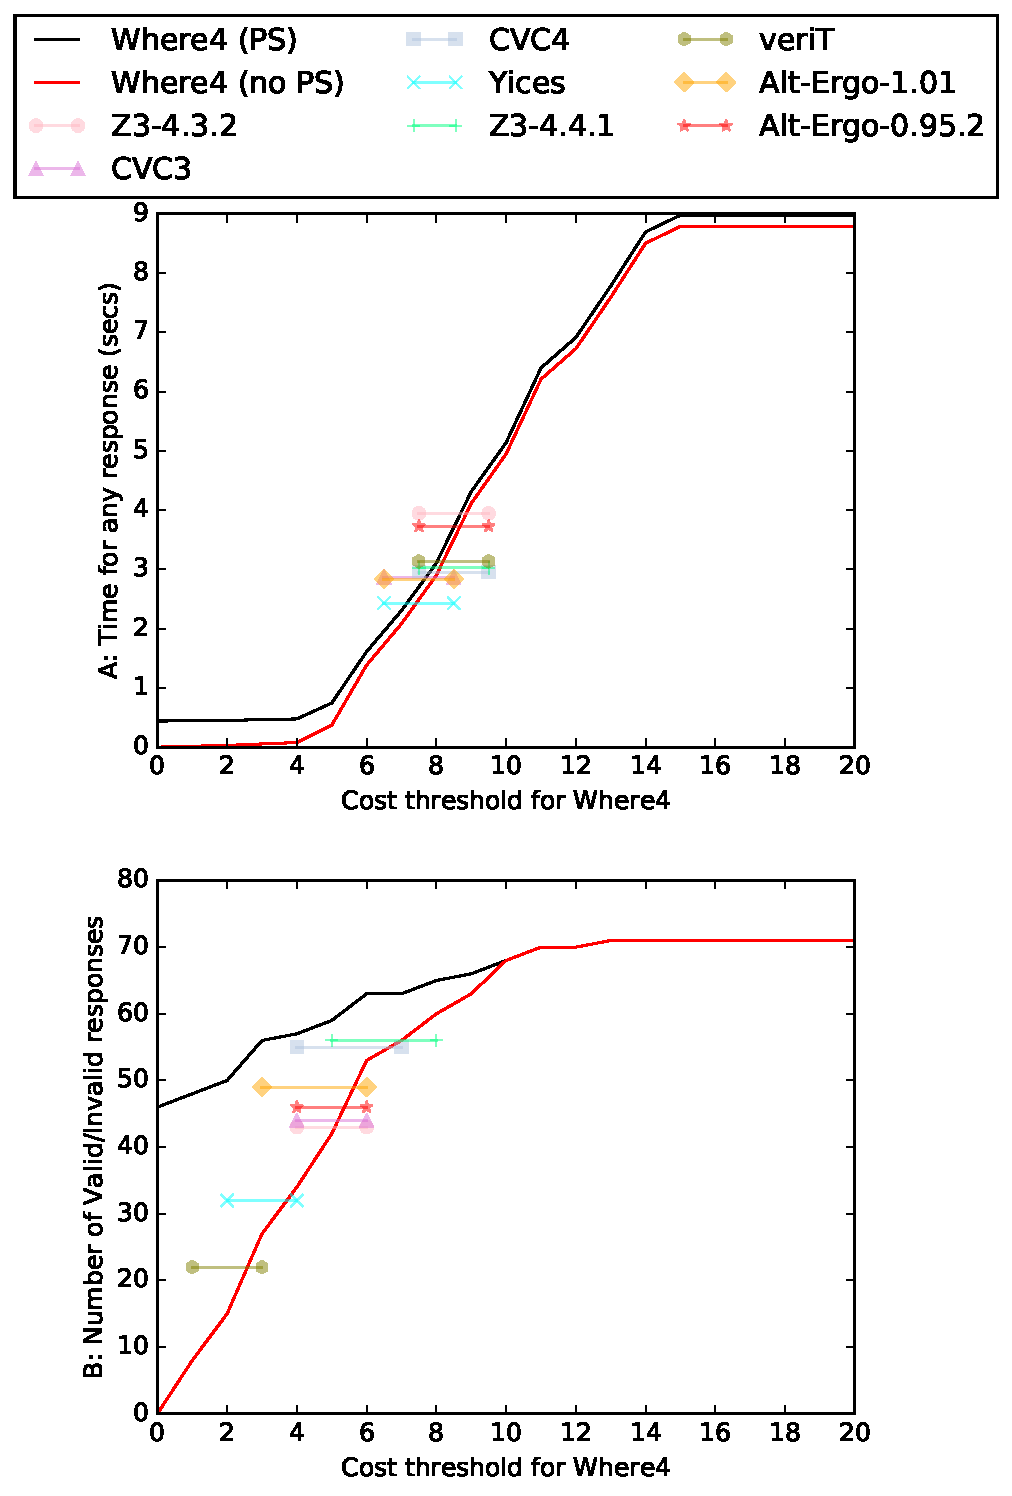
\includegraphics[width=\linewidth]{thresholds1}
	\caption[Determining a cost threshold]{Determining the appropriate value for a cost threshold (using a validation dataset). (\textit{a: top plot}) The average time taken for \where~to return an answer compared to eight SMT solvers. (\textit{b: bottom plot}) The number of Valid/Invalid answers returned by \where~compared to eight SMT solvers.}
	\label{fig:thresholds1}
\end{figure}  


\begin{figure}
	\centering
	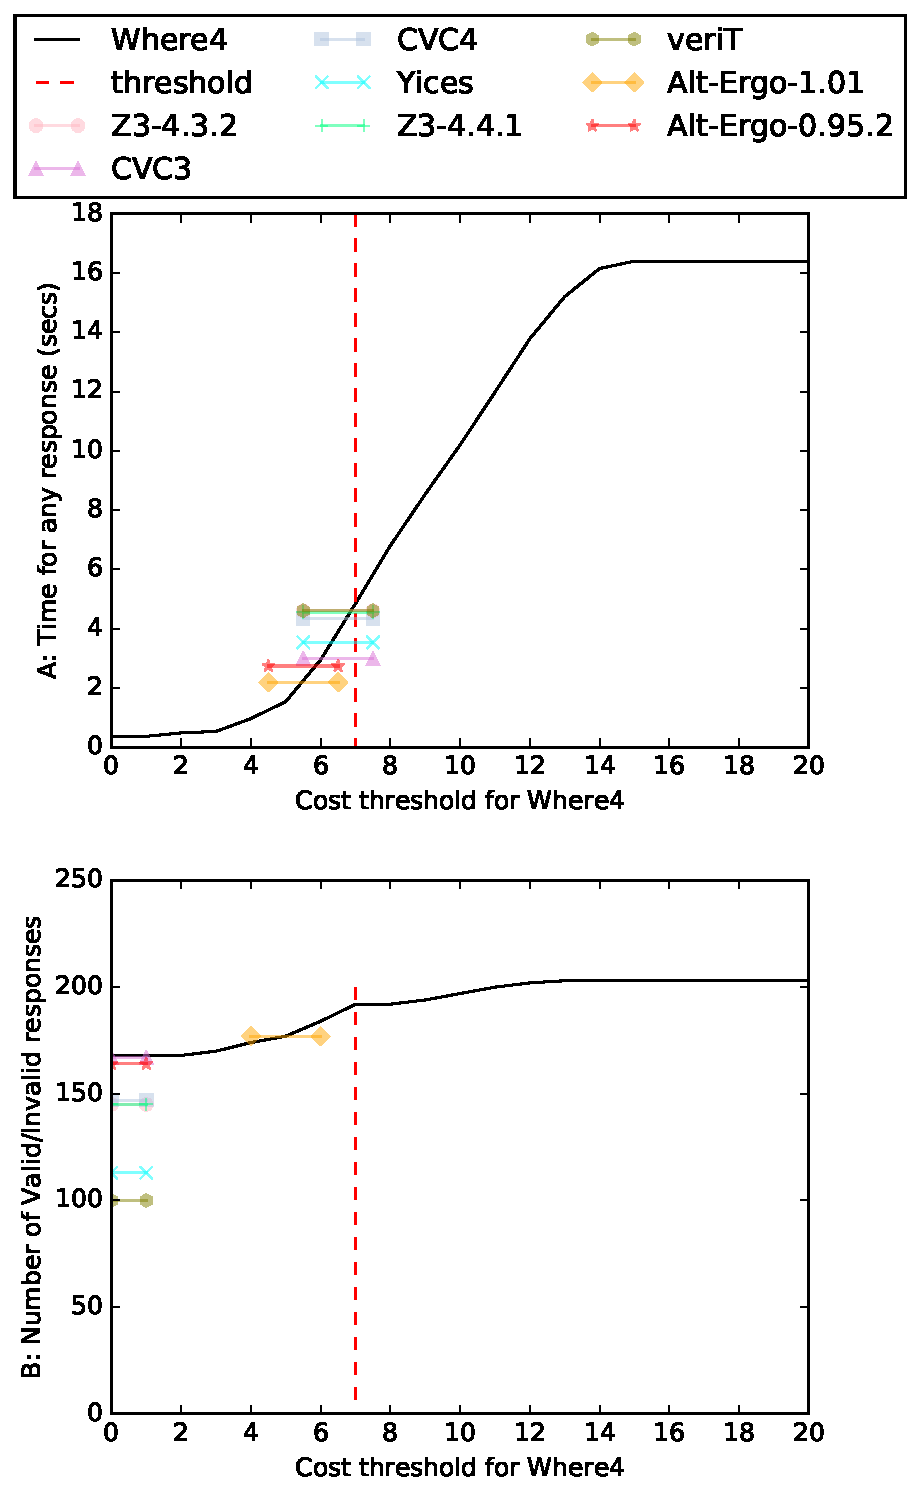
\includegraphics[width=\linewidth]{thresholds2}
	\caption[The effect of using a cost threshold]{The effect of using a cost threshold. (\textit{a: top plot}) The average time taken for \where~to return an answer compared to eight SMT solvers. (\textit{b: bottom plot}) The number of Valid/Invalid answers returned by \where~compared to eight SMT solvers.}
	\label{fig:thresholds2}
\end{figure}



Fig. \ref{fig:thresholds1}a and \ref{fig:thresholds1}b show the effect of varying this threshold when solving POs in the test set.
The top plot (\textit{a}) shows a comparison of the average time taken for \textit{any} answer to be returned (not necessarily \textit{Valid / Invalid}).
The amount of time taken by \where~often depends on the number of solvers called.
The number of solvers called depends on the cost threshold given to \where.
This is particularly true in the case where a pre-solver is not used. 
The solid black/red lines of Fig. \ref{fig:thresholds1}a, shows the increase in average time taken by \where~(with / without pre-solving) to return a response as the cost threshold increases.
Fig. \ref{fig:thresholds1}b shows the number of \textit{Valid / Invalid} responses returned by each individual SMT solver as compared to \where~with a range of threshold values.
As the corresponding results for each individual solver are unaffected by the threshold parameter, they are represented by horizontal line segments intersecting with the \where~data in Fig. \ref{fig:thresholds1}a.

We note that even when given a threshold value of zero, 46 POs are proven.
The difference with the solid red line's more gradual increase makes it obvious that the pre-solving routine is responsible for these results.
In our case, Alt-Ergo-1.01 can prove 46 POs given a time limit of one second and the solver cost is never used.
As in Fig. \ref{fig:thresholds1}a, the results for each individual solver are unaffected by the threshold parameter.

By inspecting these results, we find that a threshold value of seven gives good results.
At this threshold, the use of a pre-solver results in far more \textit{Valid/Invalid} responses being returned than the best-performing individual solver (Z3-4.4.1) and they are returned in a faster time (on average) than the fastest-returning solver (Yices).
Even without pre-solving (the solid red line), about the same number of \textit{Valid/Invalid} responses are returned as by Z3-4-4-1 and in a slightly faster time than the pre-solving version. 

As the dashed red line in Fig. \ref{fig:thresholds2} shows, a threshold value of seven also performs well on the test data.
The results for \where~using a pre-solver are shown in numerical form in Table \ref{table:threshold}. 
When \where~is given a cost threshold of five, it can prove the same number of POs as the best-performing solver -- Alt-Ergo-1.01. 
By referring to Fig. \ref{fig:thresholds2}a, we see that at the same cost threshold, it takes a shorter time to return a response, on average, than the fastest SMT solver (which is also Alt-Ergo-1.01).
If the cost threshold is increased to seven, significantly more POs can be proven. 
The average time taken to return a response is approximately equal to that of the four slowest individual solvers on the test data: CVC4, veriT, and both versions of Z3. \\
\\
\textbf{EQ1 Answer:} The cost threshold greatly improves \where's performance in comparison to the individual SMT solvers.
The performance penalties associated with portfolio solvers can be mitigated by defining a cut-off point and trusting that solvers with a predicted cost greater than this value do not need to be called.
We found this point to be about seven for the POs in the \textsf{Why3} example dataset.
Giving \where~a threshold value less than seven may result in significantly worse results without the use of a pre-solver.
The value to choose as a threshold may not be obvious in real-world scenarios with unseen results, however. 


\begin{table}
	\caption[The effect of using a cost threshold]{The effect of using a cost threshold. The average time taken for \where~(with pre-solver) to return an answer compared and the number of Valid/Invalid answers. Same data as Fig. \ref{fig:thresholds2}}
	\begin{tabularx}{0.9\textwidth}{@{}l|Z|Z|Z|Z|Z|Z@{}}

		\textsc{Threshold} & \textbf{0} & \textbf{1} & \textbf{2} & \textbf{3} & \textbf{4} & \textbf{5} \\
		\midrule
		\textbf{Avg. Time} & 0.37 & 0.37 & 0.48 & 0.53 & 0.98 & 1.77  \\
		\textbf{Num. Proved} & 168 & 168 & 168 & 169 & 173 & 177  \\
		\midrule
		\midrule
		\textsc{Threshold}  & \textbf{6} & \textbf{7} & \textbf{8} & \textbf{9} & \textbf{10} & \textbf{11}  \\
		\midrule
		\textbf{Avg. Time} & 2.72 & 4.59 & 6.55 & 8.74 & 10.31 & 11.89  \\
		\textbf{Num. Proved} & 183 & 192 & 192 & 195 & 197 & 199 \\
		\midrule
		\midrule
		\textsc{Threshold} & \textbf{12} & \textbf{13} & \textbf{14} & \textbf{15} & \textbf{16} & \textbf{17} \\
		\midrule
		\textbf{Avg. Time} & 14.16 & 15.24 & 16.06 & 16.35 & 16.35 & 16.35 \\
		\textbf{Num. Proved}  & 202 & 203 & 203 & 203 & 203 & 203 \\
		
	\end{tabularx}
	\label{table:threshold}
\end{table}

\section{EQ2: How does \where~perform in comparison to the three theoretical strategies?}


\begin{figure}
	\centering
	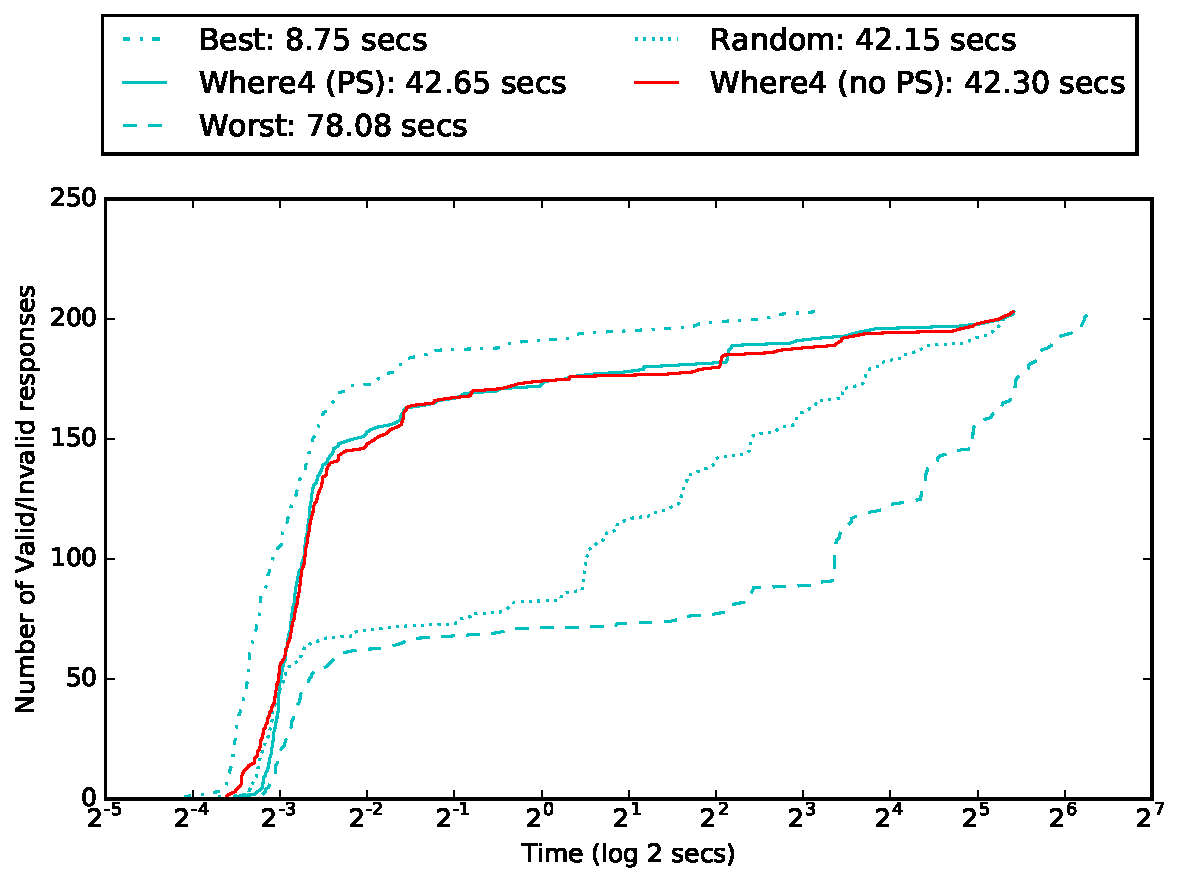
\includegraphics[width=1.0\linewidth]{line_graph_eval_provers}
	\caption{The time taken by each theoretical strategy and \where~to return all \textit{Valid/Invalid} answers in the test dataset of 263 goals}
	\label{fig:line_graph_eval_provers}
\end{figure}

Fig. \ref{fig:line_graph_eval_provers} compares the time taken for \where~(with and without the use of a Pre-Solver) and the three ranking strategies to return \textit{Valid} answers for the 263 POs in the test set.
This experiment is equivalent to running each strategy on all 263 POs in parallel and measuring the time taken for each strategy to return a total of 203 \textit{Valid} answers.
As described in Sec. \ref{sec:strategies}, \textsf{Best Ranking} and \textsf{Worst Ranking} use Alg. \ref{algo:rank} to return their time taken.
\textsf{Random Ranking}'s time measurement is based on the average of 40,320 (i.e. eight factorial, the number of individual rankings) uses of Alg. \ref{algo:rank}.
\where~(PS)'s times are derived from the use of Alg. \ref{algo:where4} with a pre-solver of Alt-Ergo-1.01. 

Although both \where~implementations and \textsf{Random Ranking} finish at approximately the same time, \where~is significantly faster for returning \textit{Valid/Invalid} answers. 
Both \where's solid lines are more closely correlated to \textsf{Best Ranking}'s rate of success than the erratic rate of the \textsf{Random Ranking} strategy.
Surprisingly, the implementation of \where~which does not use a pre-solver (Fig. \ref{fig:line_graph_eval_provers}'s solid \textit{red} line), finds slightly more \textit{Valid/Invalid} answers  at the lower end of the time scale than the pre-solver.  
We assert that this is a validation of the prediction algorithm's effectiveness: amongst provable POs, it often chooses a solver faster than the pre-solver.
Again, we find that \where~struggles to prove a small number of POs.
This trait can be seen in the amount of time needed for either \where~implementation to return all \textit{Valid/Invalid} responses (42.65/42.30 seconds) compared to that required by the \textsf{Best Ranking} strategy (just 8.75 seconds). 
\textsf{Best Ranking}'s excellent time result shows the capability of a perfect-scoring learning strategy. \\
\\
\textbf{EQ2 Answer:} At almost any point in time from zero seconds to 42.65 seconds, the number of \textit{Valid/Invalid} answers returned by \where~is greater than the number returned by \textsf{Random Ranking}.
This shows that our prediction model is a better choice than selecting a sequence of SMT solvers at random, without any regard for program features or solver capability.
\where's performance on all but the hardest POs is encouraging.
Although \where~cannot compete with \textsf{Best Ranking} yet, the performance of this theoretical strategy is motivation to further improve \where~in the future.
Over the entire test dataset (i.e. both provable and non-provable PO instances), there was no significant time time advantage associated with using a pre-solver.   



\section{EQ3: What is the time overhead of using \where~to prove \why~goals?}

\label{sec:eq3}

The timings for \where~in all plots and tables in this chapter are based solely on the performance of the constituent solvers (the measurement of which is discussed in Sec. \ref{sec:dependant}). They do not measure the time it takes for the OCaml binary to extract the static metrics, traverse the decision trees and predict the ranking. 
We have found that this adds (on average) 0.46 seconds to the time \where~takes to return a result for each of the files in the test set. 
On a per goal basis, this is equivalent to an increase in 0.056 seconds.
This overhead is only applied to goals for which pre-solving is unsuccessful.  
For the test set, pre-solving eliminated this overhead for 168 out of 263 POs (see Table \ref{table:threshold}: \where's number of \textit{Valid/Invalid} responses when the cost threshold is zero).

The imitation of an orthodox solver to interact with \why~is more costly: this is due to \why~printing each goal as a temporary file to be read in by the solver individually (see Sec. \ref{sec:why3-integration}). 
As \where~uses the abstract, internal representation of the program, the printing of each goal to the Why format is unnecessary.
The \why~driver mechanism makes this step unavoidable for any supported solver including, of course, the \where~``imitation solver''.

Another issue with calling \where~through \why~is that of applying \why's timeout value to a sequence of solver calls. 
For example, if a user gives \why~a timeout of five seconds for \where~to prove a PO and the first solver called by \where~goes over that limit, the potentially useful answer returned by the second solver in the sequence would not be returned to the user. \\
\\
\textbf{EQ3 Answer:}
While pre-solving is an important heuristic for avoiding the overhead of feature extraction and rank prediction, these processes must be optimised for \where~to be practical as a portfolio solver called from \why.   
Future work will look at a portfolio-solving \why~plugin similar to \where. Tighter integration with the \why~system can be expected to improve the efficiency of such a tool.      
In its current form, \where~is more suited to an initial proving step performed using the stand-alone command line tool.

\section{Threats to Validity}
\label{sec:threats}

In this section we discuss the threats to the validity of the evaluation presented in this chapter.
We categorise threats as either \textit{internal} or \textit{external}.
Internal threats refer to influences that can affect the response variable without the researcher's knowledge and threaten the conclusions reached about the \textit{cause} of the experimental results \cite{experimentation}. 
Threats to external validity are conditions that limit the generalisability and reproducibility of an experiment. 

\subsection{Internal}

The main threat to our work's internal validity is selection bias. All of our training and test samples are taken from the same source. 
We took care to split the data for training and testing purposes on a \textit{per file} basis, as we discussed in Sec. \ref{sub:config}. 
This ensured that \where~was not trained on a goal belonging to the same theory or file as any goal used for testing.
 
The results of running the solvers on our dataset are imbalanced: (i) there were far more \textit{Valid} responses than any other response and (ii) no goal in our dataset returned an answer of \textit{Invalid} on any of the eight solvers. 
Issue (i) could be remedied through the use of resampling.
The technique either adds copies of instances of under-represented classes (\textit{over-sampling}) or remove instances of POs returning \textit{Valid} responses (\textit{undersampling}).
A larger dataset of POs would help with resampling to ensure a representative balance of responses is reflected in the test and training set. 
Issue (ii) is a more serious problem as \where~would not be able to recognize such a goal in real-world use. 

Use of an independent dataset is likely to influence the performance of the solvers. 
Alt-Ergo was designed for use with the \why~platform -- its input language is a previous version of the Why logic language. 
It is natural that the developers of the \why~examples would write programs which Alt-Ergo in particular would be able to prove. 
Due to the syntactic similarities in input format and logical similarities such as support for type polymorphism, it is likely that Alt-Ergo would perform well with any \why~dataset. We would hope, however, that the gulf between it and other solvers would narrow.

There may be confounding effects in a solver's results that are not related to the independent variables we used (Sec. \ref{sec:independant}). 
We were limited in the tools available to extract features from the domain-specific Why logic language (in contrast to related work on model checkers which use the general-purpose C language \cite{DPVZ15:CAV, MUX} -- as previously discussed in Sec. \ref{sub:lrsvmmml}). 
We made the decision to keep the choice of independent variables simple in order to increase generalisability to other formalisms such as Microsoft's Boogie \cite{Boogie} intermediate language.  

\subsection{External}


The generalisability of our results is limited by the fact that all dependent variables were measured on a single machine.
All data collection was conducted on a single 64-bit machine running Ubuntu 14.04 with a dual-core Intel i5-4250U CPU and 16GB of RAM. 
We believe that the number of each response for each solver would not vary dramatically on a different machine of similar specifications. 
By inspecting the results when each solver was given a timeout of 60 seconds (Fig. \ref{fig:line_graph}), the rate of increase for \textit{Valid/Invalid} results was much lower than that of \textit{Unknown/Failure} results. 
The former set of results are more important when computing the cost value for each solver-goal pair.

Timings of individual goals are likely to vary widely (even across independent executions on the same machine).
% Locally, we used a statistically-accurate mean timing based on a 90\% confidence interval (see Sec. \ref{sec:dependant}). 
It is our assumption that although the actual timed values would be quite different on any other machine, the \textit{ranking} of their timings would stay relatively stable.

A ``typical'' software development scenario might involve a user verifying a single file with a small number of resultant goals: certainly much smaller than the size of our test set (263 goals). In such a setting, the productivity gains associated with using \where~would be minor. 
\where~is more suited therefore to large-scale software verification.


\section{Discussion}
\label{sec:eval-discuss}

By considering the answers to our three Evaluation Questions, we can make assertions about the success of  \where.
The answer to \textbf{EC1}, \where's performance in comparison to individual SMT solvers, is positive.
A small improvement in \textit{Valid/Invalid} responses results from using only the top-ranked solver, while a much bigger increase can be seen by making the full ranking of solvers available for use.
The time penalty associated with calling a number of solvers on an un-provable PO is mitigated by the use of a \textit{cost threshold}.
Judicious use of this threshold value can balance the time-taken-versus-goals-proved trade-off: in our test set of 263 POs, using a threshold value of seven results in 192 \textit{Valid} responses -- an increase of fifteen over the single best solver -- in a reasonable average time per PO (both \textit{Valid} and otherwise) of 4.59 seconds.

There is also cause for optimism in \where's performance as compared to the three theoretical ranking strategies -- the subject of Evaluation Question 2. 
All but the most stubborn of \textit{Valid} answers are returned in a time far better than \textsf{Random Ranking}.
We take this random strategy as representing the behaviour of the non-expert \why~user who does not have a preference amongst the variety of supported SMT solvers.
For this user, \where~could be a valuable tool in the efficient initial verification of POs through the \why~system.    

In terms of time overhead -- the concern of EQ3 -- our results are less favourable, particularly when \where~is used as an integrated part of the \why~toolchain.
The costly printing and parsing of POs slows \where~beyond the time overhead associated with feature extraction and prediction.
At present, due to the diversity of languages and input formats in use for SV (see Sec. \ref{sec:lrsv}), this is an unavoidable pre-processing step enforced by \why~(and is indeed one of the \why~system's major advantages).

Overall, we believe that the results for two out of three Evaluation Questions are encouraging and suggest a number of directions for future work to improve \where.
 

 


\chapter{Threats to Validity}
\section{Construct}
\section{Internal}
\section{External}
\section{Conclusion}

\chapter{Conclusions}
%----------------------------------------------------------------------------------------
%	THESIS CONTENT - APPENDICES
%----------------------------------------------------------------------------------------

\appendix % Cue to tell LaTeX that the following "chapters" are Appendices

% Include the appendices of the thesis as separate files from the Appendices folder
% Uncomment the lines as you write the Appendices

% Appendix A

\chapter{Python code for data analysis, statistics and learning} % Main appendix title

\label{AppendixA} % For referencing this appendix elsewhere, use \ref{AppendixA}

Write your Appendix content here.
\chapter{\where~command-line options} % Main appendix title
\thispagestyle{nohead}
\label{App:command} % For referencing this appendix elsewhere, use \ref{AppendixA}

The \textsf{Where4} command-line tool has the following functionality:
\begin{enumerate}
	\item Read in the WhyML/Why file and extract feature vectors from its goals.% formulae.
	\item Find the predicted costs for each of the 8 provers by traversing the random forest, using each goal's feature vector.
	\item Sort the costs to produce a ranking of the SMT solvers.
	\item Use the \textsf{Why3} API to call each solver (if it is installed) in rank order.
	%\item Print the result.
	\item Repeat 4 as necessary until a \textit{Valid/Invalid} response is recorded or all installed solvers have been called.
\end{enumerate}
\chapter{Pattern identification of verification programs using clustering}

%----------------------------------------------------------------------------------------
%	BIBLIOGRAPHY
%----------------------------------------------------------------------------------------

\printbibliography[heading=bibintoc]

%----------------------------------------------------------------------------------------

\end{document}  
